\documentclass[a4paper,12pt,final]{report}

% ===================================================================
%                       CORE PACKAGES
% ===================================================================
\usepackage{auxhook}
\usepackage[utf8]{inputenc}
\usepackage[T1]{fontenc}
\usepackage[french]{babel}
\usepackage{lmodern}
\usepackage{microtype}
\usepackage{geometry}

% ===================================================================
%                     DOCUMENT STRUCTURE & STYLE
% ===================================================================
\usepackage{fancyhdr}
\usepackage{titlesec}
\usepackage[nottoc]{tocbibind}
\usepackage{indentfirst}

% ===================================================================
%                      GRAPHICS, FIGURES, AND TABLES
% ===================================================================
\usepackage{graphicx}
\usepackage{pdfpages}

\usepackage{caption}
\usepackage{subcaption}
\usepackage{float}
\usepackage[section]{placeins}
\usepackage{array}
\usepackage{longtable}
\usepackage{makecell}

% ===================================================================
%                           MATH & ALGORITHMS
% ===================================================================
\usepackage{amsfonts}
\usepackage{amsmath}
\usepackage{amssymb}
\usepackage{mathrsfs}
\usepackage{siunitx}
\usepackage{algorithm}
\usepackage{algorithmic}

% ===================================================================
%                          COLOR PACKAGE
% ===================================================================
% Load xcolor EARLY with all required options
\usepackage[dvipsnames,table]{xcolor}

% ===================================================================
%                      UTILITY & SPECIAL PACKAGES
% ===================================================================
\usepackage{hyperref}
\usepackage{url}
\usepackage{dirtytalk}
\usepackage{enumitem}
\usepackage{acronym}
\usepackage{textpos}
\usepackage[pages=some]{background}

% ===================================================================
%                     CODE LISTING CONFIGURATION
% ===================================================================
\usepackage{listings}

\definecolor{codegreen}{rgb}{0,0.6,0}
\definecolor{codegray}{rgb}{0.5,0.5,0.5}
\definecolor{codepurple}{rgb}{0.58,0,0.82}
\definecolor{backcolour}{rgb}{0.95,0.95,0.92}
\definecolor{DarkGray}{rgb}{0.3,0.3,0.3}

\lstdefinestyle{mystyle}{
    backgroundcolor=\color{backcolour},   
    commentstyle=\color{codegreen},
    keywordstyle=\color{magenta},
    numberstyle=\tiny\color{codegray},
    stringstyle=\color{codepurple},
    basicstyle=\ttfamily\footnotesize,
    breakatwhitespace=false,         
    breaklines=true,                 
    captionpos=b,                    
    keepspaces=true,                 
    numbers=left,                    
    numbersep=5pt,                  
    showspaces=false,                
    showstringspaces=false,
    showtabs=false,                  
    tabsize=2
}

\lstset{style=mystyle}

% Specific language definition for YAML
\lstdefinelanguage{YAML}{
  keywords={true,false,null,y,n},
  keywordstyle=\color{DarkGray}\bfseries,
  ndkeywords={- , id, uri, predicates, filters, name, args, Path, StripPrefix, AddRequestHeader, AddResponseHeader},
  ndkeywordstyle=\color{codepurple}\bfseries,
  identifierstyle=\color{black},
  sensitive=false,
  comment=[l]{\#},
  morecomment=[s]{"}{"},
  morecomment=[s]{'}{'},
  morestring=[b]',
  morestring=[b]",
  literate =    {---}{{\char`\---}}3
                {...}{{\char`\...}}3,
}

% Specific language definition for HCL (Terraform)
\lstdefinelanguage{HCL}{
  keywords={resource, provider, variable, output, module, data, locals},
  keywordstyle=\color{blue}\bfseries,
  identifierstyle=\color{black},
  sensitive=false,
  comment=[l]{\#},
  morecomment=[s]{"}{"},
  stringstyle=\color{codepurple},
  morestring=[b]",
}

% ===================================================================
%                     CUSTOM DOCUMENT SETTINGS
% ===================================================================
\numberwithin{equation}{section}

% Page style configuration
\pagestyle{fancy}
\fancyhf{}
\cfoot{\thepage}

% ===================================================================
%                     END OF PREAMBLE
% ===================================================================
\newcommand{\euro}{\EUR\xspace}

\begin{document}

\includepdf[pages=2]{Page_Garde.pdf}

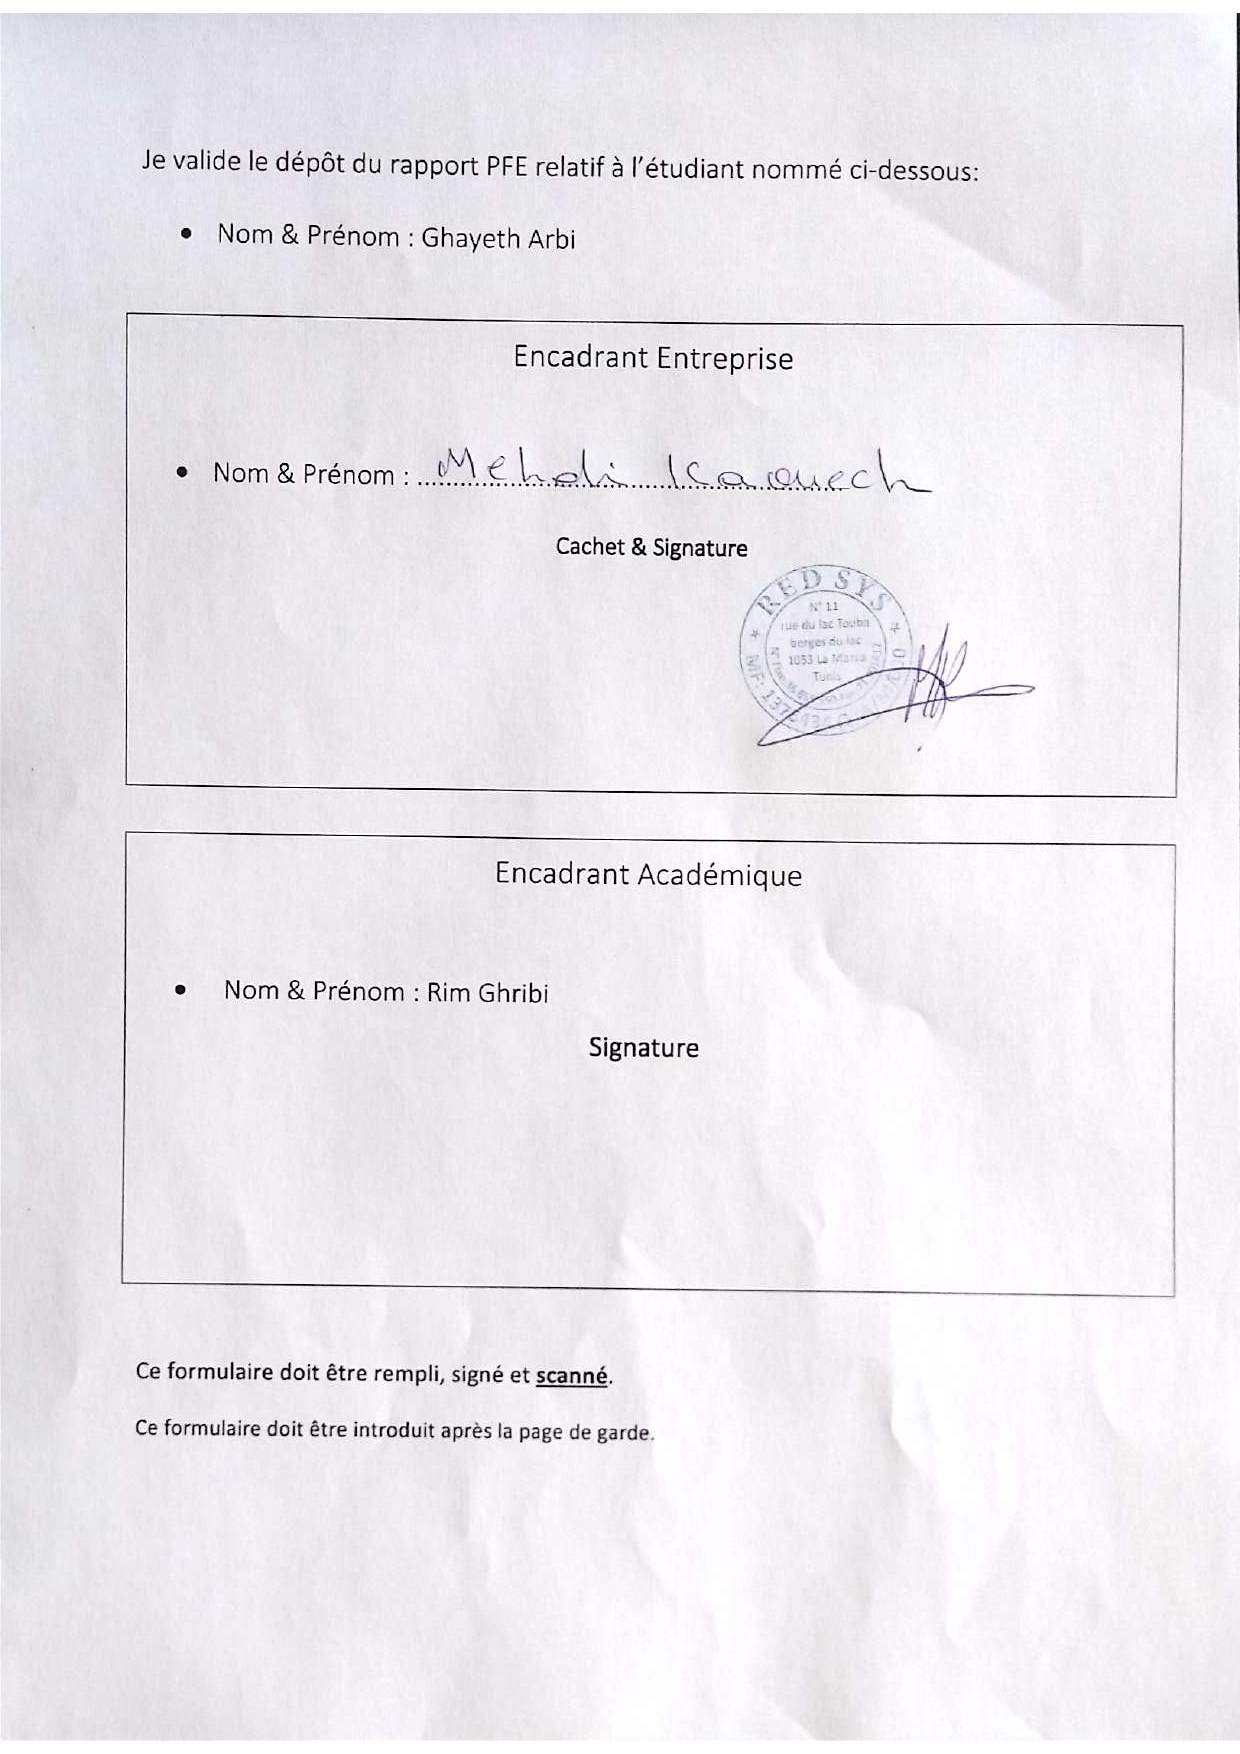
\includepdf{ss.pdf}

\newpage
\section*{Remerciements}
\vspace{1cm}

\par Avant tout, je tiens à exprimer ma profonde gratitude à ma mère pour son amour, sa patience, ses sacrifices et son soutien indéfectible tout au long de mon parcours. Ses encouragements, sa confiance et les valeurs qu'elle m'a transmises ont été une source de motivation permanente et ont largement contribué à l'aboutissement de ce projet.

\vspace{0.5cm}

\par J'adresse également mes sincères remerciements à ma tante, ainsi qu'à mes frères et sœurs, pour leur soutien, leur présence et leurs encouragements tout au long de mes études. Leur confiance et leur affection m'ont donné la force de poursuivre mes objectifs et de surmonter les difficultés rencontrées.

\vspace{0.5cm}

\par Je remercie également mes amis pour leur soutien moral, leurs conseils et les nombreux moments de partage qui ont rendu cette expérience plus agréable. Leur présence a été une véritable source de motivation tout au long de ce projet.

\vspace{0.5cm}

\par Je souhaite exprimer ma sincère reconnaissance à mon entreprise d'accueil, \textbf{RedSys}, pour m'avoir offert l'opportunité de réaliser ce Projet de Fin d'Études dans un environnement professionnel stimulant. Ce stage m'a permis de mettre en pratique les connaissances acquises au cours de ma formation, de renforcer mes compétences techniques et de participer au développement de l'application intelligente de gestion du stationnement \textbf{TuniPark}.

\vspace{0.5cm}

\par Je souhaite exprimer ma profonde gratitude envers mon superviseur chez RedSys, \textbf{M. Mehdi Kaouech}, pour son soutien, sa présence constante, sa confiance et ses conseils précieux tout au long de ce projet. L'expertise, les commentaires constructifs et le soutien toujours présent de ce dernier ont considérablement participé à l'accomplissement de ce travail.
\vspace{0.5cm}

\par Je remercie chaleureusement toute l'équipe de \textbf{RedSys} pour son accueil, sa disponibilité, son professionnalisme et l'excellente ambiance de travail qui ont rendu cette expérience particulièrement enrichissante.

\vspace{0.5cm}

\par Je tiens aussi à exprimer mes plus profonds remerciements à mon encadrante universitaire, \textbf{Mme Rim Ghribi}, pour son encadrement, sa présence constante, ses recommandations et son soutien tout au long de la pfe.
\vspace{0.5cm}

\par Enfin, je remercie toutes les personnes qui, de près ou de loin, ont contribué à la réalisation de ce projet et m'ont soutenu durant cette étape importante de mon parcours.
\chapter*{Résumé}

\par Ce mémoire présente les travaux réalisés dans le cadre d'un projet de fin d'études en vue de l'obtention du diplôme d'ingénieur en informatique. Le projet, intitulé \textbf{« TuniPark : Plateforme intelligente de gestion et de recommandation de parkings »}, a pour objectif de répondre aux difficultés rencontrées par les conducteurs lors de la recherche de places de stationnement ainsi qu'au manque de solutions numériques permettant aux propriétaires de parkings privés de gérer efficacement leurs espaces. Afin de répondre à ces problématiques, une plateforme complète composée d'une application mobile et d'une interface web d'administration a été conçue et développée. La solution permet aux utilisateurs de rechercher des parkings publics et privés, de gérer leurs sessions de stationnement, de procéder au paiement en ligne et aux propriétaires de publier et administrer leurs parkings. Elle intègre également un module d'IA basé sur un modèle \textbf{Random Forest}, capable de recommander les parkings les plus adaptés en fonction de plusieurs critères tels que la distance, la disponibilité, le comportement des utilisateurs et les tarifs proposés. Cette plateforme contribue ainsi à améliorer l'expérience utilisateur, à optimiser l'utilisation des places de stationnement et à faciliter l'administration de l'ensemble du système.

\vspace{0.5cm}

\noindent{\small \textbf{Mots-clés :} TuniPark, Gestion de parkings, Application mobile, Flutter, Angular, NestJS, PostgreSQL, Prisma, IA, Random Forest, FastAPI, Flouci, Firebase Cloud Messaging.}

\thispagestyle{empty}
\newpage

\vspace{2\baselineskip}

\tableofcontents
\thispagestyle{empty}

\listoffigures
\listoftables
\thispagestyle{empty}
\newpage

%%%%%%%%%%%%%%%%%%%%%%%%%%%%%%%%%%%%%%%%%%%%%%%%
%%%%%%%%%%%%%%%%%%%%%%%%%%%%%%%%%%%%%%%%%%%%%%%%

\chapter*{Introduction Générale}
\addcontentsline{toc}{chapter}{Introduction Générale}

\par Avec l'augmentation du nombre de véhicules et l'urbanisation croissante, la recherche d'une place de stationnement est devenue un véritable défi dans les grandes villes. Les conducteurs perdent souvent un temps considérable à chercher un parking disponible, tandis que de nombreux propriétaires de parkings privés disposent de places inoccupées qui restent inexploitées. Cette situation engendre une perte de temps, une augmentation de la consommation de carburant ainsi qu'une congestion accrue du trafic urbain.

\par Dans ce contexte, les technologies mobiles et les systèmes intelligents offrent de nouvelles opportunités pour améliorer la gestion du stationnement. En permettant la centralisation des informations, la réservation des places et l'automatisation des paiements, ces solutions contribuent à simplifier l'expérience des utilisateurs tout en optimisant l'exploitation des espaces de stationnement.

\par Ce projet de fin d'études porte sur la conception et le développement de \textbf{TuniPark}, une plateforme intelligente de gestion de parkings composée d'une application mobile destinée aux utilisateurs et d'une interface web réservée aux administrateurs. L'objectif principal du projet est de faciliter la recherche de places de stationnement publiques et privées, de permettre aux propriétaires de proposer leurs propres parkings, de gérer les sessions de stationnement et d'effectuer les paiements de manière sécurisée.

\par La solution développée intègre également un module d'IA permettant de recommander les parkings les plus pertinents en fonction de plusieurs critères, notamment la distance, le taux de disponibilité, les interactions des utilisateurs ainsi que les caractéristiques tarifaires. Cette approche tend à rendre l'expérience utilisateur plus fluide en proposant des recommandations personnalisées.

\par D'un point de vue technique, l'application mobile a été développée avec \textbf{Flutter}, tandis que l'interface d'administration a été réalisée avec \textbf{Angular}. Le Backend repose sur le framework \textbf{NestJS} et utilise \textbf{PostgreSQL} comme système de gestion de base de données via l'ORM \textbf{Prisma}. Les images sont stockées sur \textbf{Cloudinary}, les notifications Push sont assurées par \textbf{Firebase Cloud Messaging (FCM)}, les courriers électroniques sont envoyés à l'aide de \textbf{Nodemailer} et les paiements sont réalisés via la plateforme \textbf{Flouci}. Un microservice d'IA développé en \textbf{Python} avec \textbf{FastAPI} exploite un modèle \textbf{Random Forest} afin de générer les recommandations de parkings.

\par Ce mémoire présente les différentes étapes de réalisation de ce projet. Il commence par une présentation du contexte général et de l'étude de l'existant, puis décrit l'analyse des besoins, l'architecture du système et la conception. Il présente ensuite l'implémentation des différentes fonctionnalités ainsi que les tests réalisés avant de se conclure par une synthèse des résultats obtenus et des perspectives d'amélioration.

\chapter{Contexte Général et Étude Préalable}
\label{chap:general_context}


\section{Introduction}

\par Ce chapitre introductif présente le cadre général dans lequel ce projet de fin d'études a été réalisé. Il décrit dans un premier temps l'organisme d'accueil ainsi que son contexte professionnel, avant de présenter le cadre général du projet \textbf{RedSys}, en détaillant son activité, son domaine d'expertise ainsi que son environnement de travail.
\par Ensuite, le chapitre présente le contexte du projet \textbf{TuniPark}, une application conçue pour la gestion des places de stationnement. Il souligne les enjeux auxquels sont confrontés les conducteurs lorsqu'ils cherchent une place pour se garer, ainsi que les besoins qui ont conduit à l'élaboration de cette solution. Pour conclure, ce chapitre introduit la proposition de solution, les buts du projet et la méthode suivie pour réussir les diverses étapes de la conception, du développement et de la validation de l'application.


\section{Entreprise d'accueil}

\subsection{Aperçu de RedSys}

\par \textbf{RedSys} est une entreprise tunisienne spécialisée dans les technologies de l'information. Elle intervient principalement dans les domaines des infrastructures informatiques, des réseaux, du cloud et de la cybersécurité. L'entreprise a été créée par des professionnels du secteur avec l'objectif de proposer des solutions informatiques fiables, sécurisées et répondant aux besoins de ses clients.

\begin{figure}[H]
    \centering
    
\includegraphics[width=0.4\textwidth]{img/logo-enterprise.png}
    \caption{Logo de RedSys}
    \label{fig:redsys_logo}
\end{figure}

\par RedSys accompagne les entreprises dans l'intégration, le déploiement et la maintenance de leurs systèmes informatiques. Ses services concernent notamment la mise en place d'infrastructures, l'intégration de solutions réseau, la migration vers le cloud ainsi que la sécurisation des environnements numériques.

\par L'entreprise attache également une grande importance à la qualité de ses services, à la réactivité de ses équipes et à l'évolution des compétences de ses collaborateurs. Cette approche lui permet de proposer des solutions évolutives et de construire des relations durables avec ses clients.


\subsection{Domaines d'activité de RedSys}

\par RedSys accompagne les entreprises dans la conception, le déploiement et la maintenance de solutions informatiques adaptées à leurs besoins. Son activité couvre plusieurs domaines, notamment l'administration des infrastructures informatiques, les réseaux, les services cloud, la cybersécurité ainsi que le développement de solutions numériques.

\par L'entreprise intervient auprès de clients issus de différents secteurs en proposant des services de conseil, d'intégration et de support technique. Elle met également l'accent sur l'innovation et l'utilisation de technologies modernes afin de répondre aux nouveaux besoins liés à la transformation numérique.

\par Grâce à son expertise technique et à son approche orientée qualité, RedSys développe des solutions fiables et évolutives, tout en assurant un accompagnement continu de ses clients.

\subsection{Contexte organisationnel}

\par Dans le cadre de sa stratégie de développement, RedSys encourage la réalisation de projets innovants répondant à des problématiques concrètes. C'est dans cette optique qu'a été proposé le projet \textbf{TuniPark}, une application mobile et une plateforme web destinées à faciliter la gestion et la réservation des places de parking.

\par Ce projet s'inscrit dans une démarche de transformation numérique visant à optimiser l'expérience des utilisateurs en proposant une solution simple, sécurisée et accessible. Il répond également aux besoins des gestionnaires de parkings en leur offrant des outils permettant de suivre et d'administrer efficacement leurs espaces de stationnement.






\section{Cadre général du projet}

\par Le stationnement représente aujourd'hui un défi quotidien pour de nombreux conducteurs, notamment dans les zones urbaines où le nombre de places disponibles est souvent insuffisant. Cette situation engendre une perte de temps, une augmentation de la circulation ainsi qu'une consommation supplémentaire de carburant.

\par En parallèle, de nombreux espaces de stationnement privés restent inoccupés durant une partie de la journée. Ces espaces pourraient être exploités afin de répondre aux besoins des conducteurs tout en offrant une source de revenus complémentaire à leurs propriétaires.

\par Afin de répondre à cette problématique, \textbf{RedSys} a lancé le projet \textbf{TuniPark}. Dans le cadre de ce projet de fin d'études, une application mobile accompagnée d'une interface web d'administration a été conçue et développée afin de faciliter l'accès aux places de stationnement disponibles et de permettre aux propriétaires de proposer leurs espaces.

\section{Problématique}

\par Malgré l'existence de plusieurs solutions de stationnement, celles-ci ne répondent pas toujours aux besoins des conducteurs ni à ceux des propriétaires d'espaces privés. Les conducteurs rencontrent encore des difficultés pour trouver rapidement une place disponible, tandis que de nombreux propriétaires ne disposent pas d'un moyen simple et fiable pour proposer leurs espaces de stationnement.

\par La problématique de ce projet peut ainsi être formulée comme suit :

\begin{quote}
Comment développer une application permettant de faciliter l'accès aux places de stationnement disponibles tout en offrant aux propriétaires un moyen simple et sécurisé de proposer leurs espaces ?
\end{quote}

\section{Étude de l'existant}

\par Plusieurs applications permettent aujourd'hui de rechercher des parkings, de consulter leur localisation et, dans certains cas, d'effectuer un paiement en ligne. La plupart de ces solutions sont principalement orientées vers les parkings publics ou les parkings gérés par des partenaires professionnels.

\par En revanche, elles offrent rarement aux particuliers la possibilité de proposer facilement leurs propres espaces de stationnement. Cette limitation réduit le nombre de places accessibles et ne permet pas d'exploiter pleinement les espaces privés disponibles.

\section{Critique de l'existant}

\par L'étude des solutions existantes met en évidence plusieurs limites. D'une part, l'offre de stationnement reste insuffisante dans certaines zones fortement fréquentées. D'autre part, les propriétaires d'espaces privés disposent de peu d'outils leur permettant de publier et de gérer simplement leurs annonces.

\par Ces limites justifient le développement d'une solution offrant à la fois une expérience simple pour les conducteurs et un moyen efficace pour les propriétaires de mettre leurs espaces de stationnement à disposition.

\section{Solution proposée}

\par Afin de répondre aux limites identifiées lors de l'étude de l'existant, une plateforme nommée \textbf{TuniPark} a été conçue et développée. Elle se compose d'une application mobile destinée aux conducteurs et aux propriétaires de parkings privés, ainsi que d'une interface web dédiée à l'administration de la plateforme.

\begin{figure}[H]
    \centering
    
\includegraphics[width=0.28\textwidth]{img/logo-tunipark.png}
    \caption{Icône de l'application TuniPark}
    \label{fig:tunipark_icon}
\end{figure}

\par L'application mobile offre aux conducteurs la possibilité de localiser des parkings, de consulter leurs informations, d'effectuer un paiement en ligne et de gérer leurs sessions de stationnement. Les propriétaires disposent d'un espace leur permettant de publier leurs parkings, de définir les tarifs, les horaires d'ouverture, la capacité d'accueil et de suivre les revenus générés par leurs espaces.

\par L'interface web est réservée à l'administrateur de la plateforme. Elle permet d'examiner les demandes de création de parkings, de valider ou de refuser les annonces proposées et d'assurer le suivi global du fonctionnement de l'application.

\par D'un point de vue technique, l'application mobile a été développée avec \textbf{Flutter}, tandis que le backend repose sur le framework \textbf{NestJS}. Les données sont gérées à l'aide de \textbf{PostgreSQL} via l'ORM \textbf{Prisma}. La visualisation cartographique est assurée par \textbf{Mapbox} et les transactions de paiement sont réalisées grâce à la plateforme \textbf{Flouci}.
\section{Méthodologie de développement}

\subsection{Méthodologie Agile}

\par Le développement de \textbf{TuniPark} a été réalisé en adoptant la méthodologie Agile \cite{beck2001agile}. Cette approche permet de développer l'application de manière progressive tout en intégrant les retours obtenus au cours du projet.

\begin{figure}[H]
    \centering
    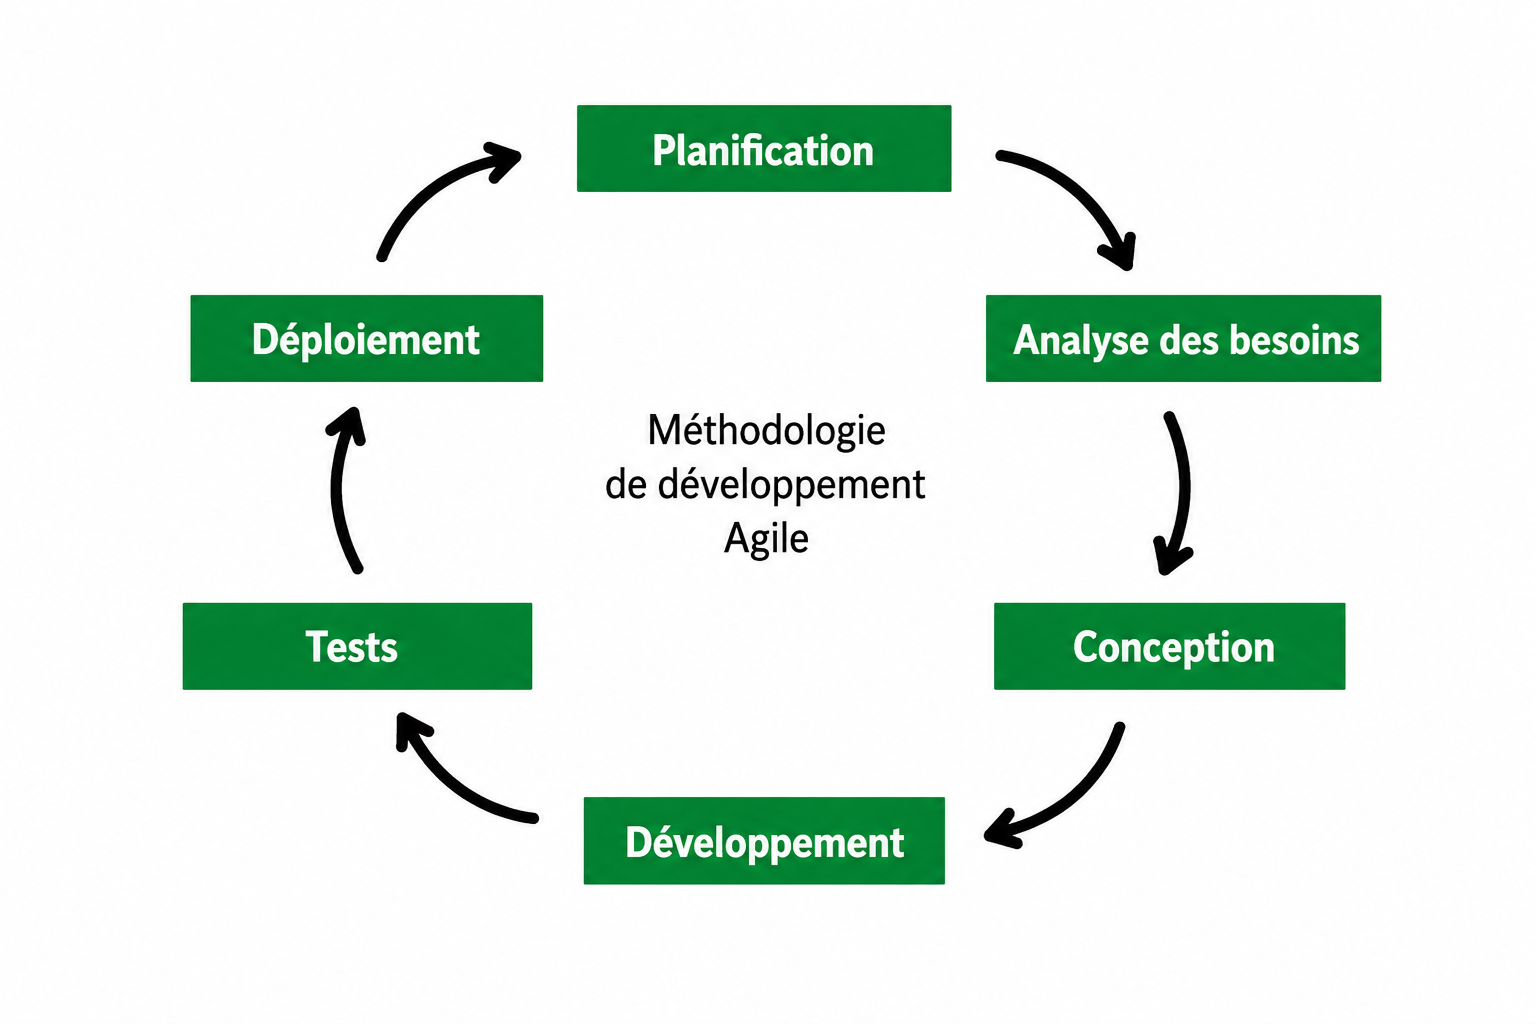
\includegraphics[width=0.75\textwidth]{img/methodologie.png}
    \caption{Cycle de développement Agile}
    \label{fig:agile_methodology}
\end{figure}

\par Comme illustré dans la Figure~\ref{fig:agile_methodology}, le développement s'est déroulé selon plusieurs phases successives : l'identification des besoins, la conception à l'aide d'UML et de l'architecture, la réalisation de l'application mobile sous Flutter, le développement du backend avec NestJS, les tests et la validation, puis le déploiement.

\par Cette organisation itérative a permis de développer progressivement les différentes fonctionnalités de l'application, de corriger rapidement les anomalies détectées et d'améliorer continuellement la solution.

\par Les principaux avantages de cette approche sont :

\begin{itemize}
    \item développement progressif de l'application ;
    \item adaptation aux évolutions des besoins ;
    \item validation régulière des fonctionnalités développées ;
    \item amélioration continue de la qualité de l'application.
\end{itemize}

\subsection{Framework SCRUM}

\par Afin d'organiser le développement, le framework SCRUM a été adopté \cite{scrum2020guide}. Les fonctionnalités de l'application ont été regroupées dans un \textit{Product Backlog} puis développées progressivement selon leur priorité.

\par Les premières itérations ont porté sur les fonctionnalités essentielles comme  l'authentification, la gestion des utilisateurs et la recherche de parkings. Les itérations suivantes ont permis d'intégrer la gestion des parkings privés, les sessions de stationnements, les paiements, les notifications ainsi que le système de recommandation basé sur l'IA.

\par À la fin de chaque itération, les fonctionnalités développées ont été testées et validées avant de procéder à la suivante. Cette organisation a permis de garantir une progression structurée du projet tout en assurant la qualité de la solution développée.

\section{Conclusion}

\par Dans ce chapitre, nous avons présenté le cadre général du TuniPark, la problématique étudiée, les solutions existantes ainsi que leurs principales limites. Nous avons ensuite proposé la solution retenue et présenté la méthodologie Agile ainsi que le framework SCRUM adoptés pour organiser le développement du projet.

\par Le chapitre suivant est consacré à l'analyse et à la spécification des besoins. Il présente les acteurs du système, les besoins fonctionnels et non fonctionnels ainsi que les principaux diagrammes UML utilisés pour la conception de l'application.
\chapter{Analyse et Spécification des Besoins}
\label{chap:requirements_analysis}

\section{Introduction}

\par Ce chapitre se concentre sur l'analyse et la spécification des besoins de l'application \textbf{TuniPark}, après avoir introduit le contexte global du projet ainsi que la solution suggérée. Cette phase consiste à repérer les différents intervenants du système, de définir les fonctionnalités attendues ainsi que les contraintes techniques et qualitatives à respecter au cours du développement.

\par Dans un premier temps, ce chapitre introduit les intervenants dans le système. Il énonce ensuite les exigences fonctionnelles et non fonctionnelles de l'application avant de présenter les diagrammes UML majeurs employés pour la modélisation du système.
\section{Identification des acteurs}

\par L'application TuniPark fait intervenir deux principaux acteurs : l'utilisateur et l'administrateur. Chacun possède des responsabilités spécifiques au sein du système.

\subsection{Utilisateur}

\par L'utilisateur représente toute personne utilisant l'application mobile. Selon son besoin, il peut agir en tant que conducteur recherchant une place de stationnement ou en tant que propriétaire souhaitant proposer un parking privé. Il peut rechercher des parkings, effectuer un paiement, démarrer une session de stationnement, publier un parking privé, consulter son historique ainsi que gérer son profil.

\subsection{Administrateur}

\par L'administrateur interagit  l'interface web afin de superviser le fonctionnement de l'application. Il est chargé de consulter les demandes de création de parkings privés, d'approuver ou de rejeter les annonces, de gérer les parkings validés et de consulter les statistiques générales de la plateforme.

\section{Besoins fonctionnels}

\par Les besoins fonctionnels décrivent les services que doit fournir l'application TuniPark.

\par L'application doit permettre à l'utilisateur de :

\begin{itemize}
    \item créer un compte et s'authentifier ;
    \item se connecter avec Google ;
    \item réinitialiser son mot de passe ;
    \item rechercher des parkings à proximité ;
    \item consulter les parkings sur une carte interactive ;
    \item afficher les informations détaillées d'un parking ;
    \item sélectionner le nombre de places souhaitées ;
    \item effectuer un paiement sécurisé via Flouci ;
    \item démarrer automatiquement une session de stationnement après le paiement ;
    \item prolonger une session de stationnement ;
    \item consulter l'historique des sessions ;
    \item recevoir des notifications ;
    \item publier un parking privé ;
    \item ajouter des photos, les informations du parking ainsi qu'un document justificatif de propriété ;
    \item définir les tarifs et les horaires d'ouverture ;
    \item modifier ou archiver un parking publié ;
    \item consulter les revenus générés par ses parkings ;
    \item gérer son profil personnel.
\end{itemize}

\par L'application doit permettre à l'administrateur de :

\begin{itemize}
    \item s'authentifier de manière sécurisée ;
    \item consulter les demandes de création de parkings privés ;
    \item approuver ou rejeter les parkings proposés ;
    \item gérer les parkings validés ;
    \item consulter les revenus et les statistiques globales ;
    \item superviser le bon fonctionnement de la plateforme.
\end{itemize}
\section{Besoins non fonctionnels}

\par Les besoins non fonctionnels définissent les exigences de qualité que doit respecter l'application.

\begin{itemize}

\item \textbf{Sécurité :} Les données des utilisateurs doivent être protégées grâce à un mécanisme d'authentification sécurisé basé sur les JSON Web Tokens (JWT). Les sessions doivent être gérées de manière sécurisée à l'aide d'un Access Token et d'un Refresh Token. Les données sensibles stockées localement doivent être protégées et supprimées automatiquement lors de l'expiration de la session. Les paiements sont réalisés via la plateforme sécurisée Flouci.

\item \textbf{Performance :} L'accès rapide aux fonctionnalités telles que la recherche de places de parking, la visualisation de la carte, les suggestions et les actions de réservation et de paiement est essentiel pour garantir une expérience utilisateur sans accroc.

\item \textbf{Fiabilité :} Il est impératif que le système assure une disponibilité élevée des services et assure l'intégrité des données relatives aux utilisateurs, aux parkings, aux réservations et aux paiements.

\item \textbf{Utilisabilité :} L'interface web d'administration et L'application mobile doivent offrir une interface intuitive, ergonomique et facile à utiliser.

\item \textbf{Scalabilité :} L'architecture doit permettre l'ajout de nouveaux utilisateurs, de nouveaux parkings ainsi que de fonctionnalités émergentes sans dégrader les performances du système.

\item \textbf{Maintenabilité :} Le code source doit être organisé de manière modulaire et respecter une architecture claire afin de faciliter la maintenance, les corrections et l'évolution de la plateforme.

\item \textbf{Compatibilité :} L'application mobile faut être compatible avec les systèmes Android et iOS, tandis que l'interface d'administration doit être accessible depuis les navigateurs web récents les plus courants.

\end{itemize}
\section{Diagramme global des cas d'utilisation}

\par Le diagramme global des cas d'utilisation présente une vue d'ensemble des principales interactions entre les acteurs et l'application \textbf{TuniPark}. Il met en évidence les principales fonctionnalités offertes par le système ainsi que les services accessibles à chaque acteur.

\begin{figure}[H]
    \centering
    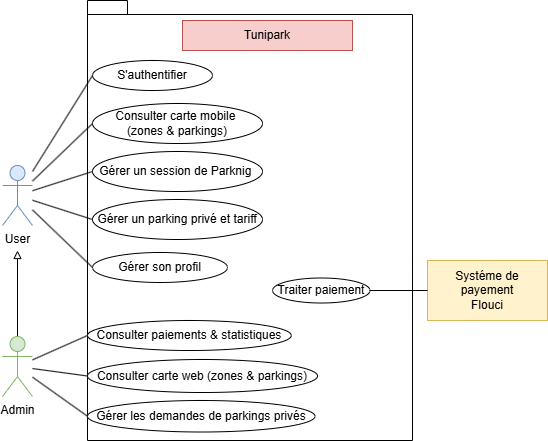
\includegraphics[width=0.95\textwidth]{img/useCase Diagram.png}
    \caption{Diagramme global des cas d'utilisation de l'application TuniPark}
    \label{fig:global_use_case}
\end{figure}

\par Comme l'illustre la Figure~\ref{fig:global_use_case}, l'utilisateur interagit avec l'application mobile afin de s'authentifier, consulter les parkings sur la carte, gérer ses sessions de stationnement, publier et administrer ses parkings privés ainsi que gérer son profil. Les opérations de paiement sont assurées par le service externe \textbf{Flouci}, intégré à l'application pour le traitement des transactions.

\par L'administrateur interagit l'interface web pour consulter la carte des parkings, gérer les demandes de création de parkings privés et accéder aux paiements ainsi qu'aux statistiques de la plateforme. Cette organisation permet de répartir clairement les responsabilités entre les différents acteurs tout en une gestion efficace du système.

\section{Description des principaux cas d'utilisation}

\par Cette section présente les principaux cas d'utilisation de l'application TuniPark. Les cas sélectionnés correspondent aux fonctionnalités essentielles proposées aux utilisateurs comme aux administrateurs, notamment la gestion des sessions de stationnement, la gestion des parkings privés, les paiements ainsi que l'administration de la plateforme.



\subsection{Authentification}

\begin{table}[H]
\centering
\renewcommand{\arraystretch}{1.25}
\begin{tabular}{|p{0.28\textwidth}|p{0.62\textwidth}|}
\hline
\textbf{Cas d'utilisation} &  Gérer l'authentification\\
\hline
\textbf{Rôle concerné} & Utilisateur, Administrateur \\
\hline
\textbf{Objectif} & Permettre à l'utilisateur ou à l'administrateur d'accéder à son espace personnel de manière sécurisée. \\
\hline
\textbf{Précondition} & L'utilisateur possède déjà un compte enregistré dans le système. \\
\hline
\textbf{Scénario principal} & L'utilisateur renseigne son adresse e-mail et son mot de passe. Le système vérifie les informations puis autorise l'accès à l'application selon le rôle de l'utilisateur. \\
\hline
\textbf{Exception} & Si les informations d'authentification sont incorrectes, Le système présente un message d'erreur et nie l'accès. \\
\hline
\textbf{Postcondition} & L'utilisateur est connecté et peut accéder aux fonctionnalités autorisées. \\
\hline
\end{tabular}
\caption{Authentification}
\label{tab:login}
\end{table}



\subsection{Gestion d'une session de parking}

\begin{table}[H]
\centering
\renewcommand{\arraystretch}{1.25}
\begin{tabular}{|p{0.28\textwidth}|p{0.62\textwidth}|}
\hline
\textbf{Cas d'utilisation} & Gérer une session de parking \\
\hline
\textbf{Rôle concerné} & Utilisateur \\
\hline
\textbf{Objectif} & Permettre à l'utilisateur de démarrer, consulter et arrêter une session de stationnement. \\
\hline
\textbf{Précondition} & L'utilisateur est authentifié et un parking est disponible. \\
\hline
\textbf{Scénario principal} & L'utilisateur sélectionne un parking, consulte ses informations, effectue le paiement puis le système démarre automatiquement la session de stationnement. \\
\hline
\textbf{Exception} & Si aucune place n'est disponible ou si une erreur survient, le système notifie l'utilisateur. \\
\hline
\textbf{Postcondition} & Une session de stationnement est créée et enregistrée. \\
\hline
\end{tabular}
\caption{Gestion d'une session de parking}
\label{tab:parking_session}
\end{table}




\subsection{Gestion d'un parking privé}

\begin{table}[H]
\centering
\renewcommand{\arraystretch}{1.25}
\begin{tabular}{|p{0.28\textwidth}|p{0.62\textwidth}|}
\hline
\textbf{Cas d'utilisation} & Gérer un parking privé \\
\hline
\textbf{Rôle concerné} & Utilisateur \\
\hline
\textbf{Objectif} & Permettre à un utilisateur de publier et gérer un parking privé ainsi que sa tarification. \\
\hline
\textbf{Précondition} & L'utilisateur est authentifié. \\
\hline
\textbf{Scénario principal} & L'utilisateur renseigne les informations du parking (adresse, nombre de places, disponibilité et tarif), puis soumet sa demande. Après validation par l'administrateur, le parking devient disponible sur la plateforme. \\
\hline
\textbf{Exception} & Si les informations sont incomplètes ou invalides, la demande est refusée jusqu'à correction. \\
\hline
\textbf{Postcondition} & Le parking est enregistré ou mis à jour dans le système. \\
\hline
\end{tabular}
\caption{Gestion d'un parking privé}
\label{tab:private_parking}
\end{table}

\subsection{Paiement d'une session}

\begin{table}[H]
\centering
\renewcommand{\arraystretch}{1.25}
\begin{tabular}{|p{0.28\textwidth}|p{0.62\textwidth}|}
\hline
\textbf{Cas d'utilisation} & Effectuer un paiement \\
\hline
\textbf{Rôle concerné} & Utilisateur \\
\hline
\textbf{Objectif} & Permettre à l'utilisateur de payer les frais de stationnement via le service Flouci. \\
\hline
\textbf{Précondition} & L'utilisateur a sélectionné un parking. \\
\hline
\textbf{Scénario principal} & Le système calcule le montant à payer selon les informations du parking. L'utilisateur est redirigé vers Flouci afin d'effectuer le paiement. Après validation de la transaction, la session de stationnement est créée automatiquement. \\
\hline
\textbf{Exception} & Si le paiement échoue ou est annulé, la transaction est marquée comme non effectuée et l'utilisateur est informé. \\
\hline
\textbf{Postcondition} & Le paiement est enregistré et la session de stationnement est démarrée. \\
\hline
\end{tabular}
\caption{Paiement d'une session}
\label{tab:payment}
\end{table}

\subsection{Validation des parkings privés}

\begin{table}[H]
\centering
\renewcommand{\arraystretch}{1.25}
\begin{tabular}{|p{0.28\textwidth}|p{0.62\textwidth}|}
\hline
\textbf{Cas d'utilisation} & Traiter les demandes de parkings privés \\
\hline
\textbf{Rôle concerné} & Administrateur \\
\hline
\textbf{Objectif} & Permettre à l'administrateur de valider ou refuser les requêtes de création de parkings privés. \\
\hline
\textbf{Précondition} & Une ou plusieurs demandes sont en attente de validation. \\
\hline
\textbf{Scénario principal} & L'administrateur consulte les demandes, vérifie les informations fournies puis accepte ou refuse la publication du parking. \\
\hline
\textbf{Exception} & Si les informations sont incomplètes ou incorrectes, la demande est rejetée avec un motif. \\
\hline
\textbf{Postcondition} & Le statut de la demande est mis à jour et l'utilisateur est informé de la décision. \\
\hline
\end{tabular}
\caption{Validation des parkings privés}
\label{tab:admin_private_parking}
\end{table}


\section{Product Backlog}

\par Ce dernier regroupe les principales fonctionnalités identifiées lors de l'analyse des besoins de l'application \textbf{TuniPark}. Il a servi de référence tout au long du développement afin de planifier les tâches, définir les priorités et organiser les différentes itérations du projet.

\par Les fonctionnalités ont été réparties selon plusieurs modules, notamment l'authentification, la gestion des parkings, les sessions de stationnement, les paiements, les notifications ainsi que l'administration de l'application.

\renewcommand{\arraystretch}{1.25}
\small

\begin{longtable}{|p{0.06\textwidth}|p{0.18\textwidth}|p{0.46\textwidth}|p{0.13\textwidth}|p{0.10\textwidth}|}
\caption{Product Backlog de l'application TuniPark}
\label{tab:product_backlog}\\

\hline
\textbf{ID} & \textbf{Module} & \textbf{User Story} & \textbf{Acteur} & \textbf{Priorité} \\
\hline
\endfirsthead

\hline
\textbf{ID} & \textbf{Module} & \textbf{User Story} & \textbf{Acteur} & \textbf{Priorité} \\
\hline
\endhead

1 & Authentification & En tant que personne utilisant l'application, mon désir est de constituer un compte pour avoir accès aux services proposés. & Utilisateur & Élevée \\
\hline

2 & Authentification & En tant qu'utilisateur, mon souhait est de me connecter en toute sécurité pour accéder à mon espace personnel. & Utilisateur / Admin & Élevée \\
\hline

3 & Authentification & Dans mon rôle d'utilisateur, je désire réinitialiser mon mot de passe via un code OTP reçu par e-mail ou téléphone. & Utilisateur & Élevée \\
\hline

4 & Carte & Dans mon rôle d'utilisateur, je désire visualiser les parkings disponibles sur une carte interactive afin de choisir celui qui me convient. & Utilisateur & Élevée \\
\hline

5 & Recherche & Dans mon rôle d'utilisateur, je désire rechercher un parking afin de trouver rapidement une place disponible. & Utilisateur & Élevée \\
\hline

6 & Session & Dans mon rôle d'utilisateur, je désire démarrer une session de stationnement après le paiement. & Utilisateur & Élevée \\
\hline

7 & Paiement & Dans mon rôle d'utilisateur, je désire payer ma session de stationnement via Flouci. & Utilisateur & Élevée \\
\hline

8 & Historique & Je souhaite, en tant qu'utilisateur, avoir la possibilité de consulter l'historique de mes sessions de stationnement. & Utilisateur & Moyenne \\
\hline

9 & Notifications & Dans mon rôle d'utilisateur, je désire recevoir des notifications concernant mes sessions et mes parkings. & Utilisateur & Moyenne \\
\hline

10 & Parking privé & Dans mon rôle d'utilisateur, je désire publier un parking privé afin de le proposer à la location. & Utilisateur & Élevée \\
\hline

11 & Parking privé & Dans mon rôle d'utilisateur, je désire ajouter des photos, une description, un tarif, des horaires et un document justificatif lors de la création d'un parking. & Utilisateur & Élevée \\
\hline

12 & Parking privé & Dans mon rôle d'utilisateur, je désire modifier ou archiver mes parkings. & Utilisateur & Moyenne \\
\hline

13 & Revenus & Dans mon rôle d'utilisateur, je désire consulter les revenus générés par mes parkings. & Utilisateur & Moyenne \\
\hline

14 & Administration & En tant qu'administrateur, je souhaite consulter les demandes de création de parkings privés. & Admin & Élevée \\
\hline

15 & Administration & En tant qu'administrateur, je souhaite approuver ou rejeter les parkings proposés. & Admin & Élevée \\
\hline

16 & Tableau de bord & En tant qu'administrateur, je souhaite consulter les statistiques générales de l'application. & Admin & Moyenne \\
\hline

17 & Revenus & En tant qu'administrateur, je souhaite consulter les revenus générés par la plateforme. & Admin & Moyenne \\
\hline

\end{longtable}

\normalsize

\par Ce Product Backlog a permis de structurer le développement de TuniPark en définissant les fonctionnalités à implémenter selon leur priorité. Les fonctionnalités critiques, notamment l'authentification, la gestion des parkings, les sessions de stationnement et les paiements, ont été développées en priorité. Les fonctionnalités complémentaires, comme les notifications, les statistiques et la gestion des revenus, ont ensuite été intégrées afin d'enrichir l'application et d'améliorer l'expérience utilisateur.

\section{Conclusion}

\par Ce chapitre a présenté l'analyse et la spécification des besoins de l'application \textbf{TuniPark}. Il a permis d'identifier les différents acteurs du système, de définir les besoins fonctionnels et non fonctionnels, ainsi que de présenter le diagramme global des cas d'utilisation.

\par Les principaux cas d'utilisation ont ensuite été décrits afin de mieux comprendre les interactions entre les utilisateurs, l'administrateur et l'application. Enfin, le Product Backlog a été établi pour organiser les fonctionnalités à développer et définir leurs priorités.

\par Le prochain chapitre portera sur la conception et à l'architecture de l'application. Il présentera l'architecture générale du système, les choix techniques adoptés, la modélisation de la base de données ainsi que les différents diagrammes UML utilisés lors de la conception.
\chapter{Conception et Architecture du Système}
\label{chap:system_design_architecture}

\section{Introduction}

\par Après avoir examiné les exigences fonctionnelles et non fonctionnelles de \textbf{TuniPark}, cette étape consiste à définir l'architecture du système ainsi que les choix techniques retenus pour son développement. L'objectif est de concevoir une architecture modulaire, évolutive et facilement maintenable, capable de répondre aux différents besoins de l'application.

\par Ce chapitre présente tout d'abord l'architecture générale du système, puis décrit les architectures logique et physique. Les principales technologies utilisées sont ensuite présentées avant d'introduire la conception de la base de données ainsi que les principaux diagrammes UML réalisés durant la phase de conception.
\section{Architecture du système}

\par L'application \textbf{TuniPark} repose sur une architecture client--serveur composée d'une application mobile destinée aux utilisateurs, d'une interface web réservée à l'administrateur, d'un serveur Backend, d'un microservice d'IA ainsi que d'une base de données relationnelle. Cette architecture assure une séparation claire entre les différentes couches du système afin d'améliorer la maintenabilité, la sécurité et l'évolutivité de l'application.

    \subsection{Architecture logique}

    \par Cette partie décrit les principaux composants logiciels de l'application ainsi que leurs interactions. Le système est organisé en cinq couches : la couche de présentation, la couche métier, la couche d'accès aux données, la couche de données et la couche des services externes.

\par La couche de présentation comprend l'application mobile développée avec \textbf{Flutter} \cite{flutter}, destinée aux utilisateurs, ainsi que l'interface web d'administration développée avec \textbf{Angular} \cite{angular}. L'application mobile permet notamment de rechercher des parkings, gérer des sessions de stationnement, publier des parkings privés, effectuer des paiements, consulter les statistiques personnelles et recevoir des notifications. L'interface web permet à l'administrateur de superviser les utilisateurs, les parkings, les paiements et les différentes informations de la plateforme.

\par La couche métier est implémentée à l'aide du framework \textbf{NestJS} \cite{nestjs}. Elle expose une API REST sécurisée et regroupe l'ensemble de la logique métier de l'application. Cette couche est composée de plusieurs modules, notamment l'authentification, la gestion des utilisateurs, des parkings, des sessions de stationnement, des parkings privés, des paiements, des notifications, des statistiques ainsi que du système de recommandation basé sur l'IA.

\par La couche d'accès aux données repose sur \textbf{Prisma ORM} \cite{prisma}. Celui-ci facilite les échanges entre le Backend et la base de données PostgreSQL tout en garantissant une manipulation fiable et sécurisée des données.

\par La couche de données fait appel à une base de données de type relationnel \textbf{PostgreSQL} \cite{postgresql}. Elle assure le stockage des informations relatives aux utilisateurs, aux parkings, aux sessions de stationnement, aux paiements, aux notifications ainsi qu'aux interactions exploitées par le système de recommandation.

\par Enfin, l'application s'appuie sur plusieurs services externes. Les images des parkings sont stockées sur \textbf{Cloudinary} \cite{cloudinary}, les notifications Push sont envoyées grâce à \textbf{Firebase Cloud Messaging (FCM)} \cite{firebase}, les paiements électroniques sont réalisés via \textbf{Flouci} \cite{flouci}, les courriers électroniques sont envoyés à l'aide de \textbf{Nodemailer} \cite{nodemailer}, tandis que l'envoi des codes OTP par SMS est prévu via \textbf{Twilio} \cite{twilio}. Un microservice développé avec \textbf{FastAPI} \cite{fastapi} héberge également le modèle d'IA basé sur l'algorithme \textbf{Random Forest} \cite{breiman2001randomforest}, chargé de calculer les recommandations de parkings.

\begin{figure}[H]
    \centering
    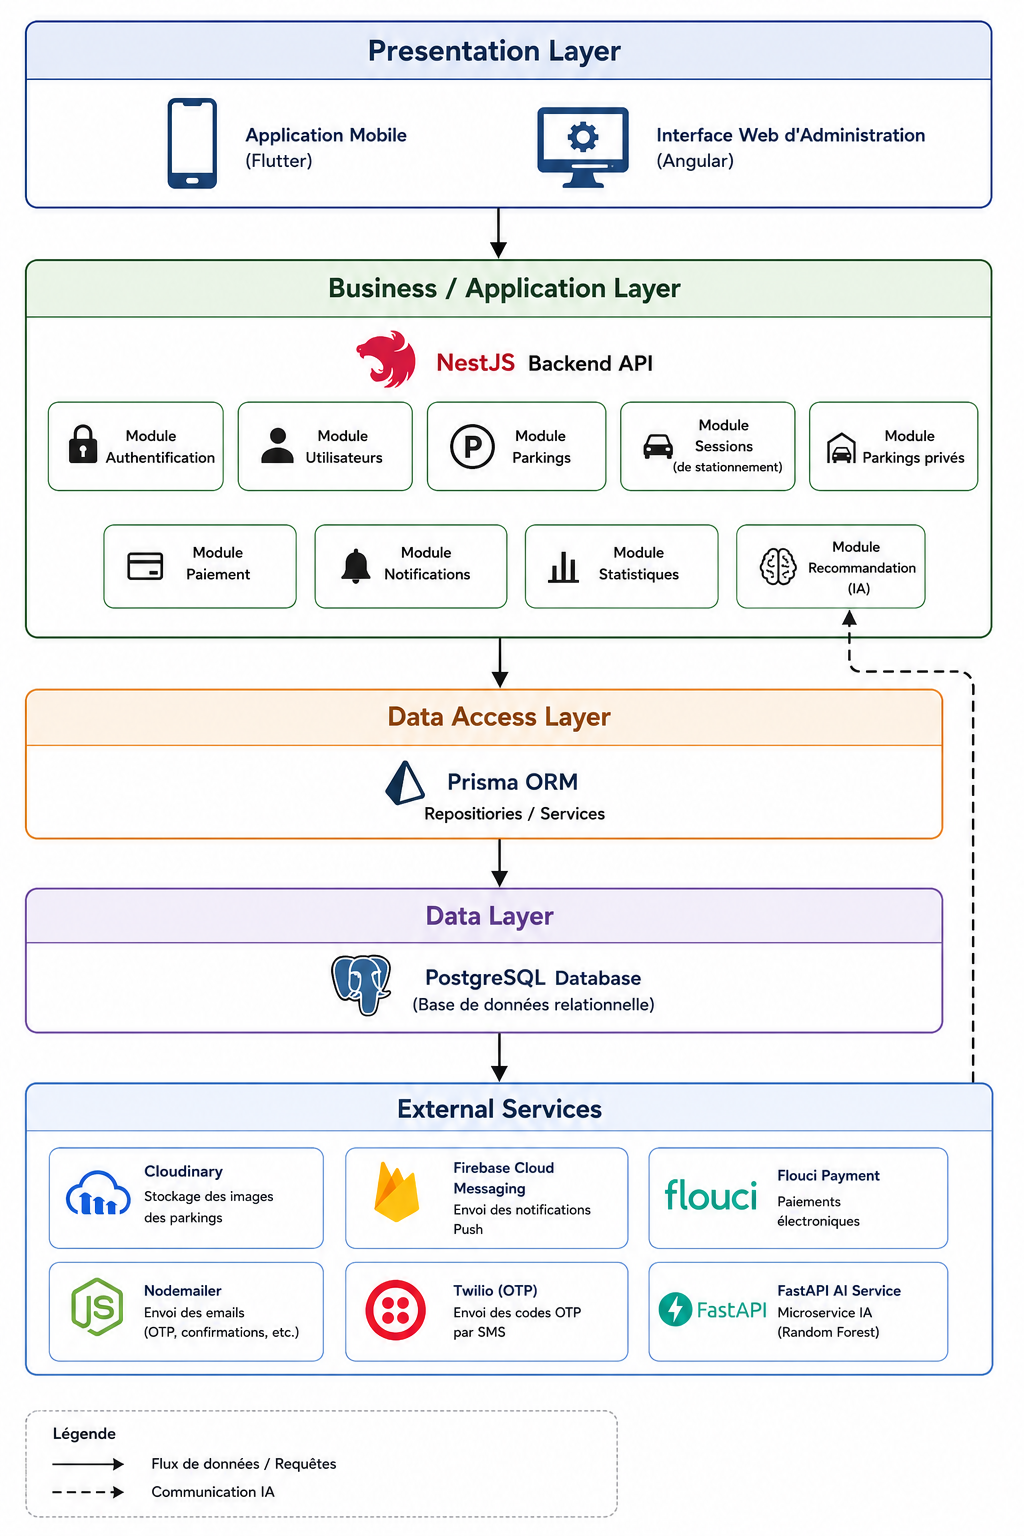
\includegraphics[width=0.60\textwidth]{img/architecturelogi.png}
    \caption{Architecture logique de TuniPark}
    \label{fig:logical_architecture}
\end{figure}

\par Comme l'illustre la Figure~\ref{fig:logical_architecture}, les interfaces mobile et web communiquent avec le Backend via des requêtes REST sécurisées. Le Backend centralise la logique métier, interagit avec PostgreSQL par l'intermédiaire de Prisma ORM et communique avec les différents services externes tels que Cloudinary, Flouci, Firebase Cloud Messaging, Nodemailer ainsi que le microservice d'IA développé avec FastAPI.
\subsection{Architecture physique}

\par Cette architecture présente le déploiement réel des différents composants de l'application TuniPark. Le système est accessible à travers deux interfaces clientes : l'application mobile développée avec \textbf{Flutter} et l'interface web d'administration développée avec \textbf{Angular}.

\par L'interface web d'administration est hébergée sur \textbf{Vercel} \cite{vercel}, tandis que le Backend développé avec \textbf{NestJS}, le microservice d'IA développé avec \textbf{FastAPI} ainsi que la base de données \textbf{PostgreSQL} sont déployés sur \textbf{Render} \cite{render}. Les interfaces clientes communiquent avec le Backend au moyen de requêtes HTTPS vers une API REST sécurisée.

\par Le Backend centralise la logique métier de l'application et assure la communication avec la base de données ainsi qu'avec les différents services externes. Les images des parkings sont stockées sur \textbf{Cloudinary}, les notifications Push sont envoyées via \textbf{Firebase Cloud Messaging}, les paiements électroniques sont traités par \textbf{Flouci} et les courriers électroniques sont envoyés à l'aide de \textbf{Nodemailer}.

\par Le service \textbf{Twilio} est prévu pour l'envoi des codes OTP par SMS, mais il n'est pas encore opérationnel dans la version actuelle de l'application. Le microservice FastAPI héberge le modèle de recommandation basé sur l'algorithme Random Forest et communique avec le Backend NestJS à travers des requêtes HTTP.

\begin{figure}[H]
    \centering
    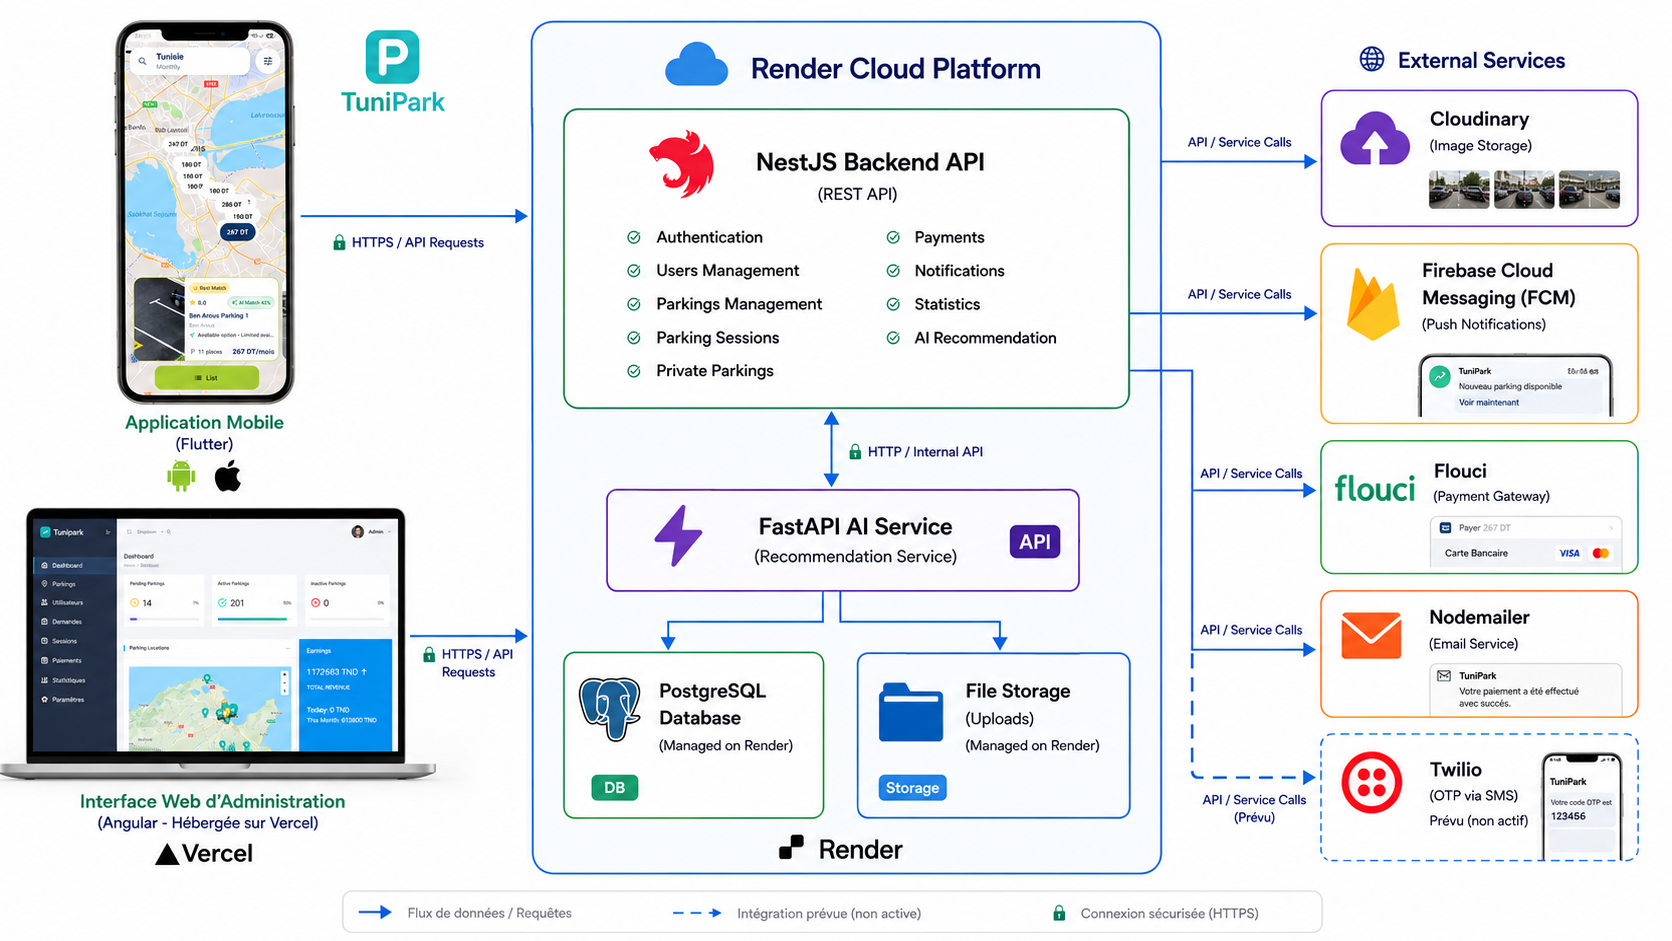
\includegraphics[width=0.95\textwidth]{img/physique.png}
    \caption{Architecture physique de l'application TuniPark}
    \label{fig:physical_architecture}
\end{figure}

\par Comme le montre la Figure~\ref{fig:physical_architecture}, les différents composants sont déployés sur des services Cloud distincts. Cette séparation permet de simplifier le déploiement, de faciliter la maintenance et de faire évoluer indépendamment le Backend, l'interface web et le service d'IA.
\section{Choix techniques}

\par Les technologies retenues pour le développement de l'application \textbf{TuniPark} ont été sélectionnées en fonction des exigences du projet, notamment en matière de performance, de sécurité, de maintenabilité et d'évolutivité. L'objectif était de mettre en place une architecture moderne, reposant sur des outils fiables, afin de concevoir une application mobile, une interface web d'administration, un Backend sécurisé et une base de données performante, tout en assurant l'interfaçage avec des services externes et un système de recommandation basé sur l'IA.\subsection{Flutter}

\par Flutter \cite{flutter} a été choisi pour développer l'application mobile de TuniPark. Ce framework développé par Google permet de concevoir une application multiplateforme à partir d'une seule base de code, compatible avec Android et iOS.

\par L'application mobile permet aux utilisateurs de rechercher des parkings, consulter leur disponibilité sur une carte interactive, démarrer et arrêter une session de stationnement, effectuer des paiements, gérer leurs parkings privés ainsi que recevoir des notifications en temps réel.

\begin{figure}[H]
    \centering
    
\includegraphics[width=0.12\textwidth]{img/flutter_logo.png}
    \caption{Logo du framework Flutter}
\end{figure}

\subsection{Angular}

\par Angular \cite{angular} a été utilisé pour développer l'interface web d'administration de TuniPark. Cette application permet à l'administrateur de superviser la plateforme, gérer les utilisateurs, valider les demandes de parkings privés, consulter les statistiques ainsi que suivre l'ensemble des opérations réalisées sur le système.

\par L'application Angular communique avec le Backend via des API REST sécurisées.

\begin{figure}[H]
    \centering
    
\includegraphics[width=0.15\textwidth]{img/angular.png}
    \caption{Logo du framework Angular}
\end{figure}

\subsection{NestJS}

\par Le Backend de TuniPark a été développé avec NestJS \cite{nestjs}. Ce framework basé sur Node.js et TypeScript offre une architecture modulaire facilitant l'organisation des différents modules de l'application.

\par Il centralise la logique métier du système, notamment l'authentification, la gestion des utilisateurs, des parkings, des sessions de stationnement, des paiements, des notifications, ainsi que la communication avec le microservice d'IA.

\begin{figure}[H]
    \centering
    
\includegraphics[width=0.22\textwidth]{img/nestjs_logo.png}
    \caption{Logo du framework NestJS}
\end{figure}

\subsection{PostgreSQL et Prisma}

\par Les données de TuniPark sont stockées dans une base de données relationnelle PostgreSQL \cite{postgresql}. Cette solution garantit l'intégrité des données, une gestion fiable des liens entre les entités, ainsi que de bonnes performances lors des requêtes.
\par L'accès à la base de données est assuré par Prisma ORM \cite{prisma}, qui simplifie les opérations de création, de lecture, de modification et de suppression des données tout en offrant une sécurité de typage grâce à TypeScript.

\begin{figure}[H]
   \centering
   
\includegraphics[width=0.16\textwidth]{img/postgresql_logo.png}
    \caption{Logo de PostgreSQL}
\end{figure}


\subsection{FastAPI et Random Forest}

\par Pour offrir une meilleure expérience aux utilisateurs, TuniPark intègre un microservice d'IA développé avec FastAPI \cite{fastapi} en Python. Ce service expose des API REST consommées par le Backend NestJS.

\par Le modèle de recommandation repose sur l'algorithme Random Forest \cite{breiman2001randomforest}. Il analyse plusieurs critères tels que la distance entre l'utilisateur et le parking, le taux de disponibilité, le taux de conversion des consultations en réservations, le taux de prolongation des sessions ainsi que le tarif du parking afin de calculer un score de recommandation.

\par Les parkings sont ensuite classés selon ce score afin de proposer en priorité les emplacements les plus pertinents pour chaque utilisateur.

\begin{figure}[H]
    \centering
    
\includegraphics[width=0.15\textwidth]{img/python_logo.png}
    \caption{Microservice IA développé avec FastAPI}
\end{figure}

\subsection{Authentification JWT}

\par La sécurisation des accès repose sur JSON Web Token (JWT) \cite{jwt}. Après une authentification réussie, le Backend génère un Access Token valide pendant une heure ainsi qu'un Refresh Token valide pendant trois jours.

\par Lorsque l'Access Token expire, un intercepteur Dio renouvelle automatiquement celui-ci à l'aide du Refresh Token sans intervention de l'utilisateur. Si le Refresh Token arrive également à expiration, la session est automatiquement fermée, les informations locales sont supprimées et l'utilisateur est orienté vers la page de connexion.

\begin{figure}[H]
    \centering
    
\includegraphics[width=0.10\textwidth]{img/jwt_logo.png}
    \caption{Authentification basée sur JWT}
\end{figure}

\subsection{Cloudinary}

\par Cloudinary \cite{cloudinary} est utilisé pour le stockage des images des parkings. Ce service Cloud permet d'héberger les images, de les optimiser automatiquement et de fournir des liens sécurisés pour leur affichage dans l'application.

\begin{figure}[H]
    \centering
    
\includegraphics[width=0.18\textwidth]{img/cloudinary_logo.png}
    \caption{Logo de Cloudinary}
    \label{fig:cloudinary_logo}
\end{figure}

\subsection{Firebase Cloud Messaging}

\par Firebase Cloud Messaging (FCM) \cite{firebase} permet l'envoi de notifications Push aux utilisateurs. Il est utilisé pour informer les utilisateurs des validations de leurs parkings, des paiements, des rappels de session ainsi que des différentes notifications générées par l'application.
\begin{figure}[H]
    \centering
    
\includegraphics[width=0.18\textwidth]{img/firebase_logo.png}
    \caption{Logo de Firebase Cloud Messaging}
    \label{fig:fcm_logo}
\end{figure}



\subsection{Flouci}

\par Flouci \cite{flouci} est la solution de paiement électronique intégrée à TuniPark. Elle permet aux utilisateurs d'effectuer leurs paiements de manière sécurisée directement depuis l'application mobile avant le démarrage d'une session de stationnement.

\begin{figure}[H]
    \centering
    
\includegraphics[width=0.18\textwidth]{img/flouci_logo.png}
    \caption{Logo de Flouci}
    \label{fig:flouci_logo}
\end{figure}


\subsection{Nodemailer}

\par Nodemailer \cite{nodemailer} est utilisé pour l'envoi automatique des courriers électroniques, notamment lors de la création d'un compte, de la changement de mot de passe et de l'envoi des codes OTP par courrier électronique.

\begin{figure}[H]
    \centering
    
\includegraphics[width=0.18\textwidth]{img/nodemailer_logo.png}
    \caption{Logo de Nodemailer}
    \label{fig:nodemailer_logo}
\end{figure}


\section{Conception de la base de données}

\par La base de données de l'application \textbf{TuniPark} repose sur le SGBD relationnelles \textbf{PostgreSQL} \cite{postgresql}. Elle est structurée autour de plusieurs tables correspondant aux principaux domaines fonctionnels de l'application, notamment la gestion des utilisateurs, des parkings, des sessions de stationnement, des paiements, des notifications et des interactions utilisées par le système de recommandation.

\par L'accès aux données est assuré par \textbf{Prisma ORM} \cite{prisma}, qui facilite la définition des relations entre les entités et les opérations réalisées depuis le Backend NestJS. Cette organisation permet de préserver la cohérence des données et de faciliter l'évolution du système.

\subsection{Tables de gestion des utilisateurs et des accès}

\begin{table}[H]
\centering
\small
\renewcommand{\arraystretch}{1.25}
\begin{tabular}{|p{0.28\textwidth}|p{0.62\textwidth}|}
\hline
\textbf{Table} & \textbf{Rôle dans l'application} \\
\hline
\texttt{User} & Sauvegarde les informations des utilisateurs, notamment leur identité, leurs coordonnées, leur mot de passe, leur rôle ainsi que l'état de vérification de leur adresse électronique et de leur numéro de téléphone. Cette table contient également les informations temporaires nécessaires à la vérification et à la changement de mot de passe par code OTP. \\
\hline
\texttt{FcmToken} & Stocke les jetons Firebase associés aux appareils des utilisateurs afin de permettre l'envoi de notifications Push. Un utilisateur peut posséder plusieurs jetons lorsqu'il utilise plusieurs appareils. \\
\hline
\end{tabular}
\caption{Tables de gestion des utilisateurs et des accès}
\label{tab:user_access_tables}
\end{table}

\subsection{Tables de gestion des parkings}

\begin{table}[H]
\centering
\small
\renewcommand{\arraystretch}{1.25}
\begin{tabular}{|p{0.28\textwidth}|p{0.62\textwidth}|}
\hline
\textbf{Table} & \textbf{Rôle dans l'application} \\
\hline
\texttt{Parking} & Stocke les informations principales d'un parking, notamment son titre, son type, sa description, son emplacement, ses horaires d'ouverture, ses photos, ses caractéristiques, le nombre total de places et le nombre de places disponibles. Elle conserve également son statut de validation ainsi que la référence de son propriétaire. \\
\hline
\texttt{Tariff} & Stocke les informations tarifaires associées à un parking, telles que le prix par unité, par jour ou par mois, ainsi que les durées minimale et maximale autorisées. Chaque parking possède au maximum un tarif. \\
\hline
\end{tabular}
\caption{Tables de gestion des parkings}
\label{tab:parking_tables}
\end{table}

\subsection{Tables de gestion des sessions de stationnement}

\begin{table}[H]
\centering
\small
\renewcommand{\arraystretch}{1.25}
\begin{tabular}{|p{0.28\textwidth}|p{0.62\textwidth}|}
\hline
\textbf{Table} & \textbf{Rôle dans l'application} \\
\hline
\texttt{ParkingSession} & Stocke les sessions de stationnement ouvertes par les utilisateurs. Elle contient le parking sélectionné, les informations du véhicule, la date de début, la date de fin, la durée payée ainsi que le statut de la session. \\
\hline
\end{tabular}
\caption{Table de gestion des sessions de stationnement}
\label{tab:parking_session_table}
\end{table}

\subsection{Table de gestion des paiements}

\begin{table}[H]
\centering
\small
\renewcommand{\arraystretch}{1.25}
\begin{tabular}{|p{0.28\textwidth}|p{0.62\textwidth}|}
\hline
\textbf{Table} & \textbf{Rôle dans l'application} \\
\hline
\texttt{Payment} & Stocke les paiements associés aux sessions de stationnement. Elle conserve le fournisseur de paiement, le montant, le statut de la transaction, la référence retournée par le fournisseur ainsi que la date de confirmation du paiement. \\
\hline
\end{tabular}
\caption{Table de gestion des paiements}
\label{tab:payment_table}
\end{table}

\subsection{Tables de gestion des notifications}

\begin{table}[H]
\centering
\small
\renewcommand{\arraystretch}{1.25}
\begin{tabular}{|p{0.28\textwidth}|p{0.62\textwidth}|}
\hline
\textbf{Table} & \textbf{Rôle dans l'application} \\
\hline
\texttt{Notification} & Stocke les notifications destinées aux utilisateurs, notamment leur titre, leur contenu, leur type, les données complémentaires ainsi que leur état de lecture. \\
\hline
\texttt{FcmToken} & Associe chaque appareil à un jeton Firebase afin de transmettre les notifications Push au bon utilisateur. \\
\hline
\end{tabular}
\caption{Tables liées aux notifications}
\label{tab:notification_tables}
\end{table}

\subsection{Table utilisée par le système de recommandation}

\begin{table}[H]
\centering
\small
\renewcommand{\arraystretch}{1.25}
\begin{tabular}{|p{0.28\textwidth}|p{0.62\textwidth}|}
\hline
\textbf{Table} & \textbf{Rôle dans l'application} \\
\hline
\texttt{ParkingInteraction} & Enregistre les interactions réalisées par les utilisateurs avec les parkings. Les interactions prises en charge sont la consultation d'un parking, le démarrage d'une session et la prolongation d'une session. Ces données permettent de calculer les taux de conversion et de prolongation exploités par le système de recommandation. \\
\hline
\end{tabular}
\caption{Table utilisée par le système de recommandation}
\label{tab:recommendation_table}
\end{table}
























\subsection{Diagramme de classes}

\par Le schéma de classes décrit la configuration globale de l'application \textbf{TuniPark}. Il souligne les entités clés du système, leurs caractéristiques ainsi que les liens qui les unissent. Le modèle couvre notamment la gestion des utilisateurs, des parkings, des sessions de stationnement, des paiements, des notifications et des interactions utilisées par le système de recommandation.

\begin{figure}[H]
    \centering
    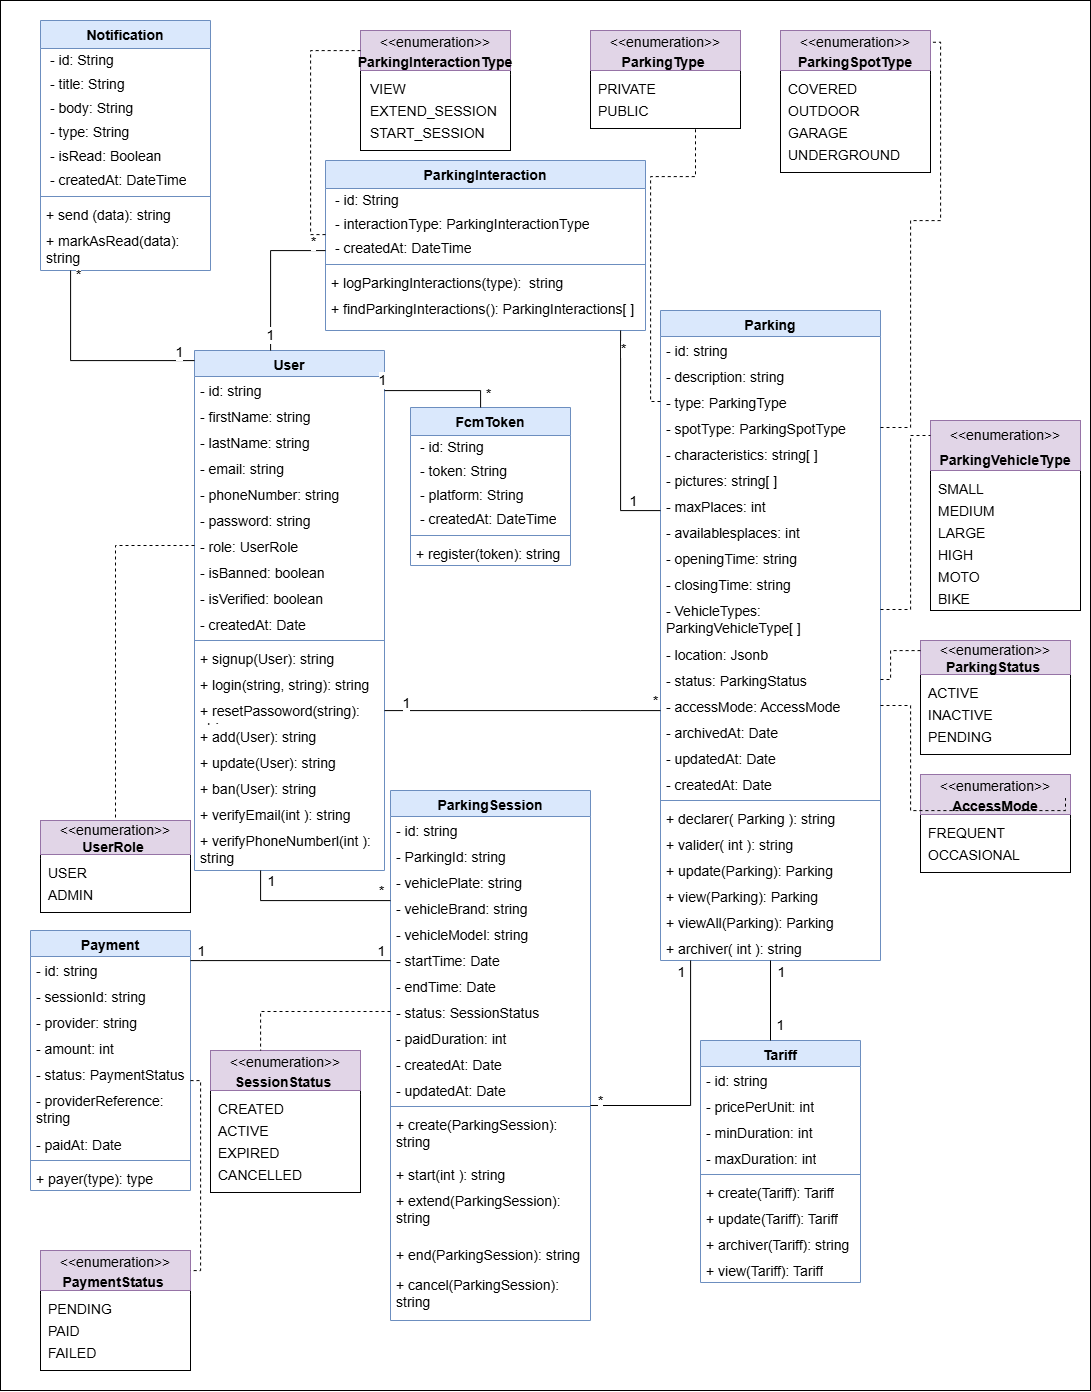
\includegraphics[width=1\textwidth]{img/class diag.drawio.png}
    \caption{Diagramme de classes de l'application TuniPark}
    \label{fig:class_diagram}
\end{figure}

\par Comme illustré dans la Figure~\ref{fig:class_diagram}, l'entité \textbf{User} occupe une place centrale dans le système. Elle contient les informations personnelles et les données nécessaires à l'authentification, ainsi que le rôle attribué à chaque utilisateur. Un utilisateur peut posséder plusieurs parkings, ouvrir plusieurs sessions de stationnement, recevoir des notifications et générer différentes interactions avec les parkings.

\par L'entité \textbf{Parking} regroupe les informations descriptives d'un espace de stationnement, notamment son type, son emplacement, ses horaires d'ouverture, ses caractéristiques, ses images, sa capacité et son statut. Chaque parking appartient à un propriétaire et peut être associé à plusieurs sessions de stationnement et interactions. Une relation individuelle relie également chaque parking à son tarif, représenté par l'entité \textbf{Tariff}.

\par L'entité \textbf{ParkingSession} représente une session de stationnement ouverte par un utilisateur dans un parking donné. Elle contient les informations du véhicule, les dates de début et de fin, la durée payée ainsi que l'état de la session. Une session peut être associée à un seul paiement, stocké dans l'entité \textbf{Payment}, qui conserve le montant, le fournisseur, le statut de la transaction et sa référence externe.

\par Les entités \textbf{Notification} et \textbf{FcmToken} prennent en charge l'envoi et le suivi des notifications. Enfin, l'entité \textbf{ParkingInteraction} enregistre les actions réalisées sur les parkings, telles que la consultation, le démarrage ou la prolongation d'une session. Ces données sont exploitées pour calculer les indicateurs utilisés par le système de recommandation.

\section{Diagrammes de séquence}

\par Les diagrammes de séquence permettent de représenter le comportement dynamique de l'application TuniPark. Ils illustrent les échanges entre les différents acteurs, l'application mobile, l'interface web d'administration, le serveur Backend, la base de données ainsi que les services externes tels que Flouci, Firebase Cloud Messaging et le microservice d'IA.

\subsection{Diagramme de séquence de l'authentification}


\par Ce diagramme met en évidence la démarche d'authentification d'un utilisateur au sein de l'application \textbf{TuniPark}. Après avoir saisi son adresse électronique ou son numéro de téléphone ainsi que son mot de passe, l'application mobile envoie une requête d'authentification au Backend. Celui-ci vérifie l'existence de l'utilisateur dans la base de données, contrôle la validité des informations d'identification puis génère un \textit{Access Token} et un \textit{Refresh Token} \cite{jwt}. Les jetons générés sont ensuite retournés à l'application et stockés de manière sécurisée sur l'appareil afin de permettre l'accès aux fonctionnalités protégées. En cas d'informations d'identification invalides, un message d'erreur est renvoyé à l'utilisateur et l'authentification est refusée.

\begin{figure}[H]
    \centering
    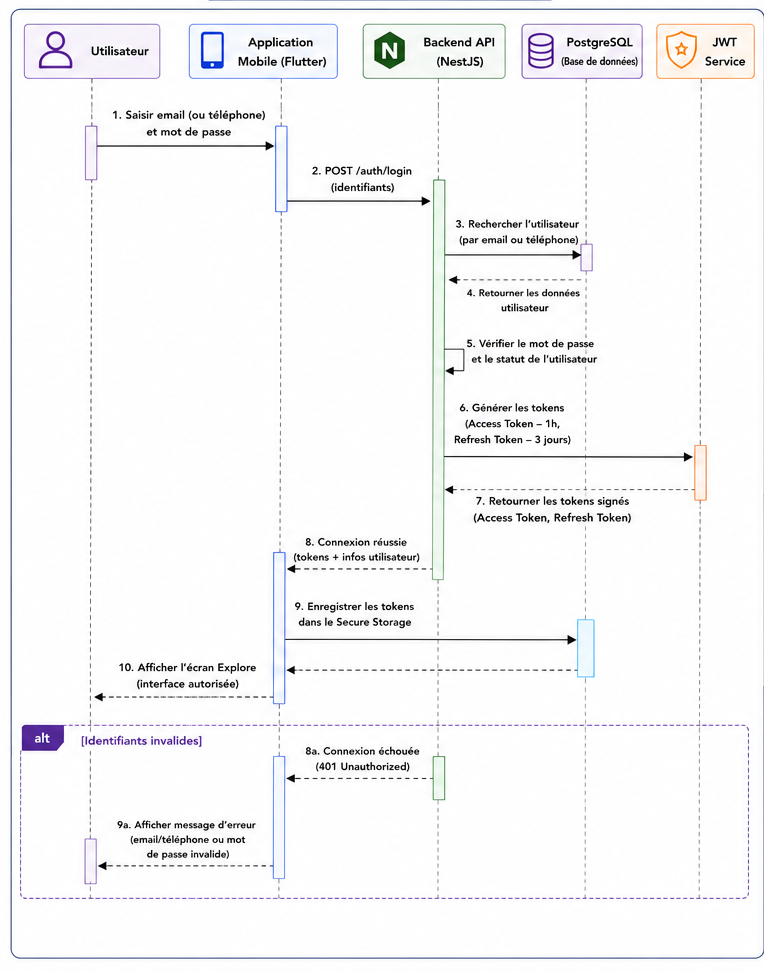
\includegraphics[width=0.95\textwidth]{img/aauth.png}
    \caption{Authentification}
    \label{fig:sequence_authentication}
\end{figure}
  
\subsection{Diagramme de séquence du renouvellement automatique du jeton}

\par Ce diagramme illustre le mécanisme de renouvellement automatique de l'\textit{Access Token}. Lorsqu'une requête retourne une réponse indiquant l'expiration du jeton d'accès, l'application utilise le \textit{Refresh Token} précédemment enregistré afin de demander un nouveau jeton au Backend. Après validation du \textit{Refresh Token}, le Backend génère un nouvel \textit{Access Token} qui est enregistré dans le stockage sécurisé de l'application. La requête initiale est ensuite relancée de manière transparente, sans intervention de l'utilisateur. Si le \textit{Refresh Token} est invalide ou expiré, les jetons sont supprimés et l'utilisateur est automatiquement redirigé vers l'écran de connexion.

\begin{figure}[H]
    \centering
    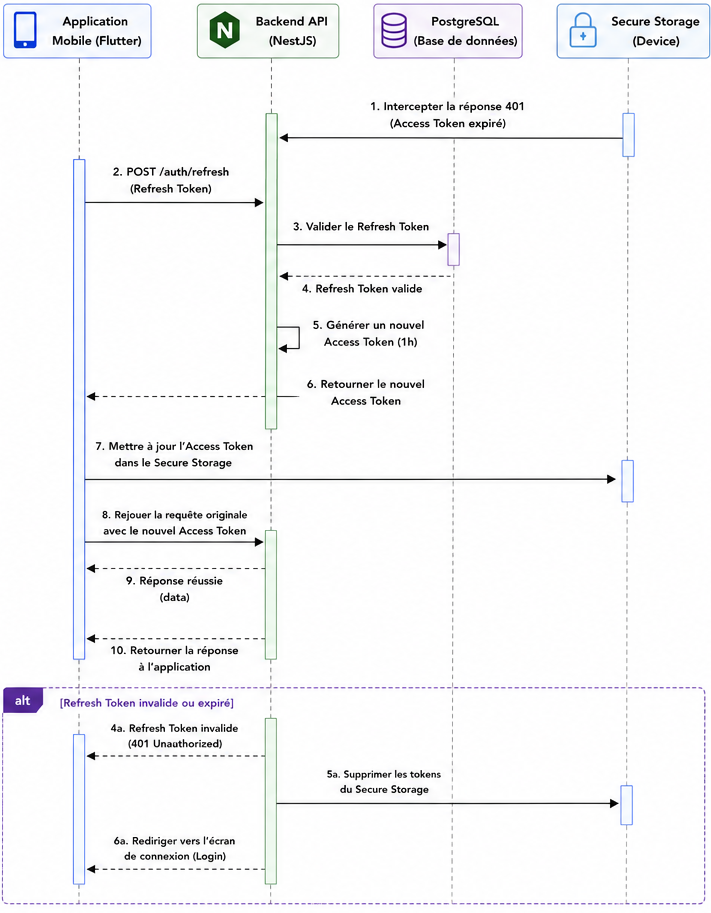
\includegraphics[width=0.7\textwidth]{img/refreshht.png}
    \caption{Renouvellement automatique du jeton}
    \label{fig:sequence_refresh_token}
\end{figure}

\subsection{Diagramme de séquence de la création d'une session de stationnement}

\par Ce diagramme illustre le processus de création d'une session de stationnement dans l'application \textbf{TuniPark}. Après avoir sélectionné un parking et renseigné les informations nécessaires, telles que la durée souhaitée, le véhicule et le numéro d'immatriculation, l'utilisateur soumet une demande de création de session. Le Backend vérifie alors la disponibilité du parking dans la base de données, crée une nouvelle session avec le statut \texttt{CREATED} et enregistre les informations correspondantes. Les détails de la session sont ensuite retournés à l'application mobile afin d'afficher un récapitulatif avant le paiement.

\begin{figure}[H]
    \centering
    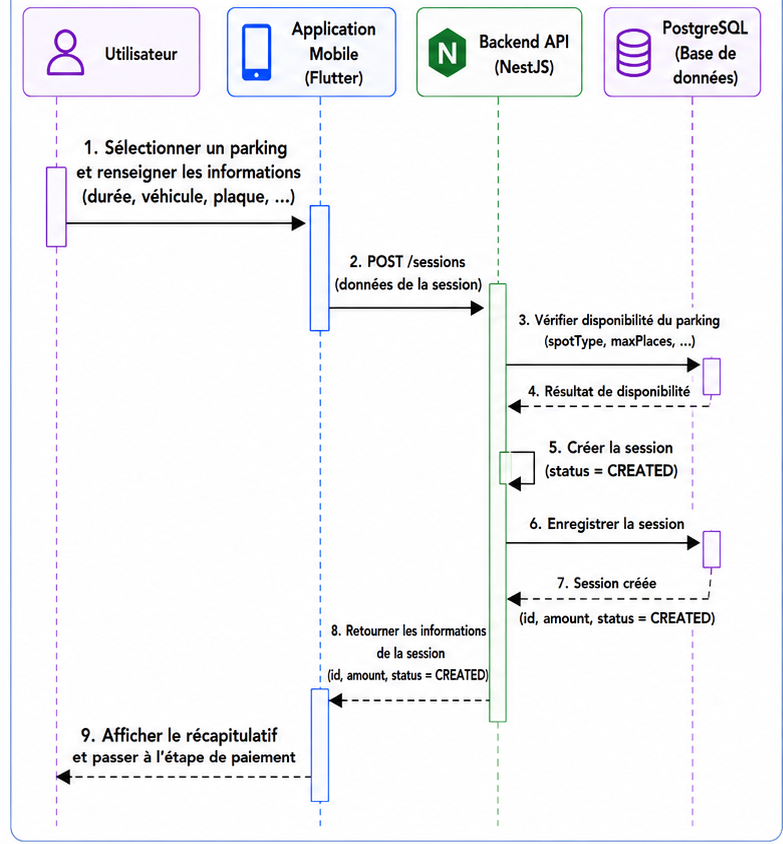
\includegraphics[width=0.65\textwidth]{img/session_creation_sequence.png}
    \caption{Création d'une session de stationnement}
    \label{fig:sequence_session_creation}
\end{figure}

\subsection{Diagramme de séquence du paiement d'une session de stationnement}

\par Ce diagramme présente le processus de paiement d'une session de stationnement à l'aide de la passerelle de paiement \textbf{Flouci} \cite{flouci}. Après validation du récapitulatif, l'utilisateur est renvoyé vers l'interface de paiement sécurisée de Flouci afin d'effectuer la transaction. Une fois le paiement terminé, Flouci transmet automatiquement le résultat au Backend via un \textit{Webhook}. En cas de succès, le Backend met à jour l'état du paiement, active la session de stationnement en changeant son statut de \texttt{CREATED} à \texttt{ACTIVE} et envoie une notification de confirmation à l'utilisateur. Si le paiement échoue ou est annulé, le paiement est marqué comme échoué, la session conserve son statut \texttt{CREATED} et l'application informe l'utilisateur afin qu'il puisse réessayer ultérieurement.

\begin{figure}[H]
    \centering
    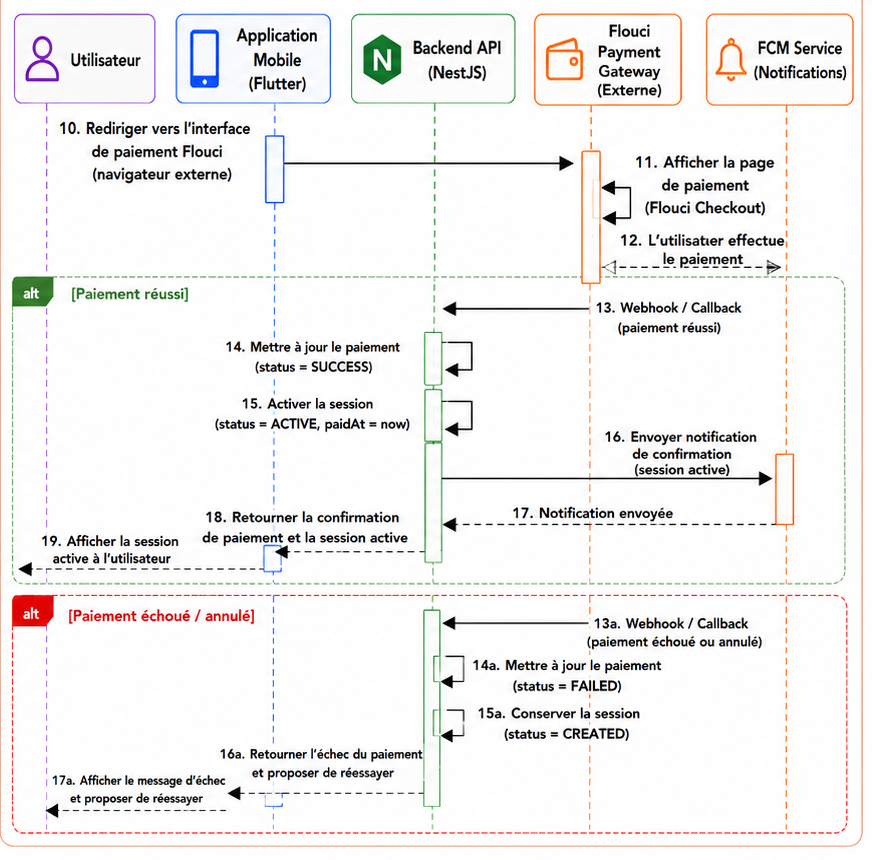
\includegraphics[width=0.85\textwidth]{img/session_payment_sequence.png}
    \caption{Paiement d'une session de stationnement}
    \label{fig:sequence_session_payment}
\end{figure}
\subsection{Diagramme de séquence de la recommandation intelligente des parkings}

\par Ce diagramme illustre le fonctionnement du système de recommandation des parkings. Après avoir obtenu la position de l'utilisateur, l'application envoie une requête au Backend. Celui-ci récupère les parkings disponibles ainsi que leurs statistiques d'utilisation, puis transmet les caractéristiques de chaque parking au microservice d'IA développé avec FastAPI \cite{fastapi}. Le modèle Random Forest \cite{breiman2001randomforest} calcule un score de recommandation pour chaque parking et retourne les résultats au Backend, qui les trie avant de les renvoyer à l'application mobile. En cas d'indisponibilité du microservice, le Backend applique automatiquement un algorithme de secours basé sur des règles afin d'assurer la continuité du service.

\begin{figure}[H]
    \centering
    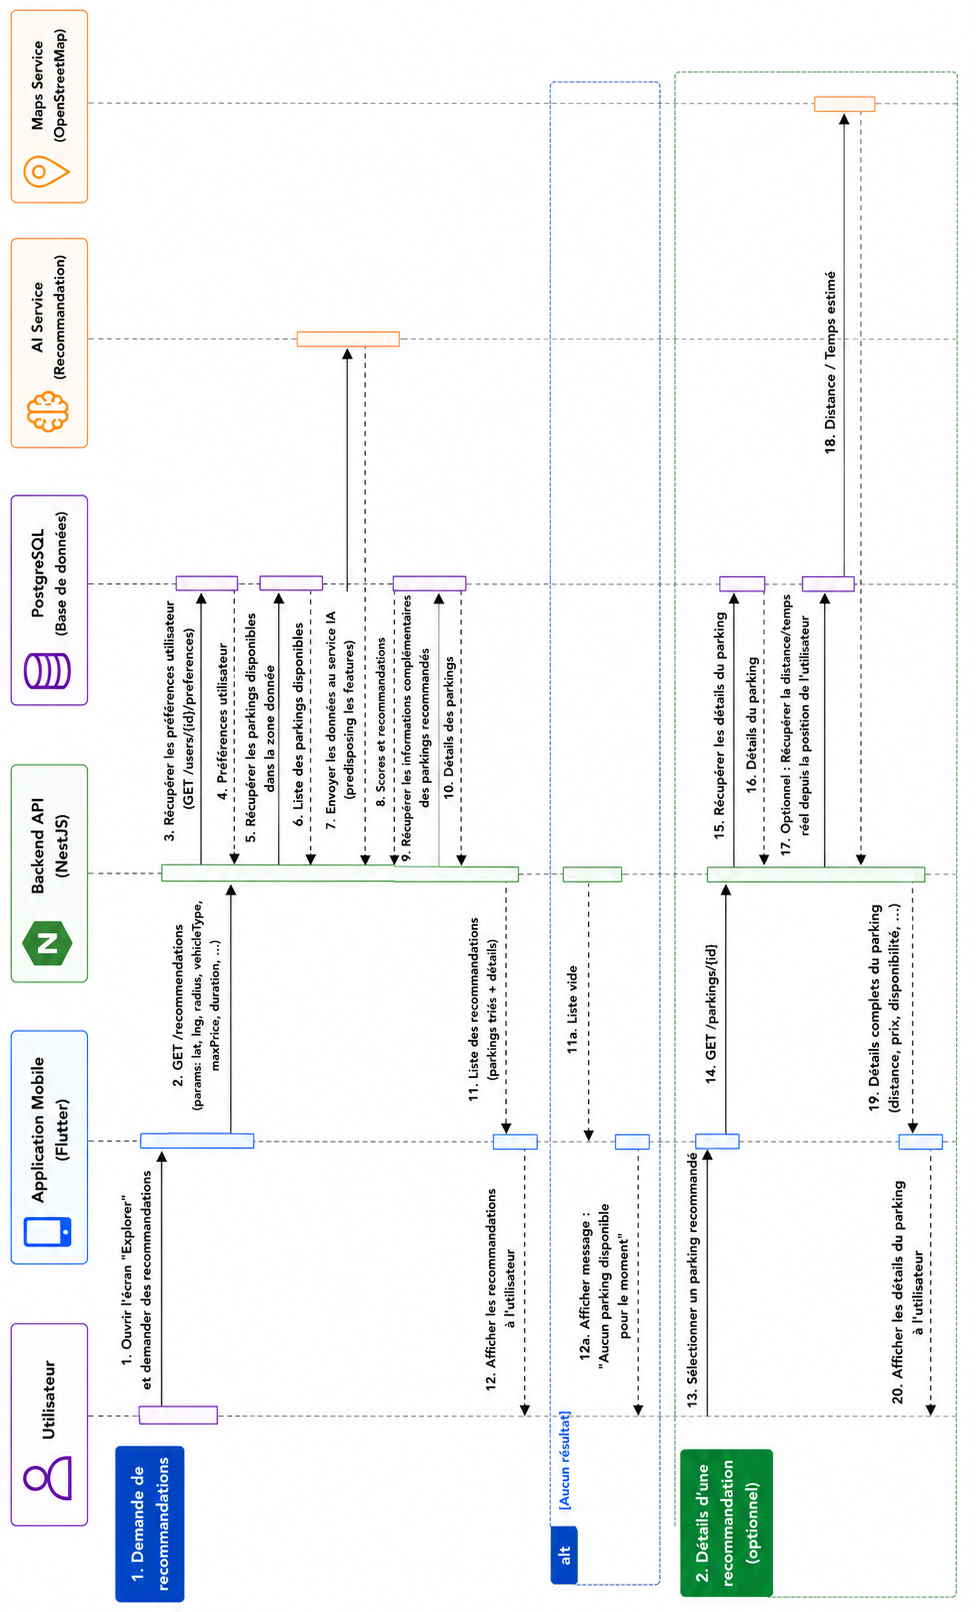
\includegraphics[width=1\textwidth]{img/ai_recom_seq.png}
    \caption{Recommandation intelligente des parkings}
    \label{fig:sequence_ai}
\end{figure}

\subsection{Diagramme de séquence de l'ajout d'un parking privé}

\par Ce diagramme présente le processus permettant à un propriétaire de proposer un parking privé sur la plateforme TuniPark. Après avoir renseigné les informations du parking et téléversé les images, l'application transmet la demande au Backend. Celui-ci vérifie les données, enregistre le parking avec le statut \textit{PENDING} puis le rend disponible dans l'interface d'administration pour validation. Après examen, l'administrateur accepte ou rejette la demande. Le propriétaire est ensuite informé de la décision par une notification.

\begin{figure}[H]
    \centering
    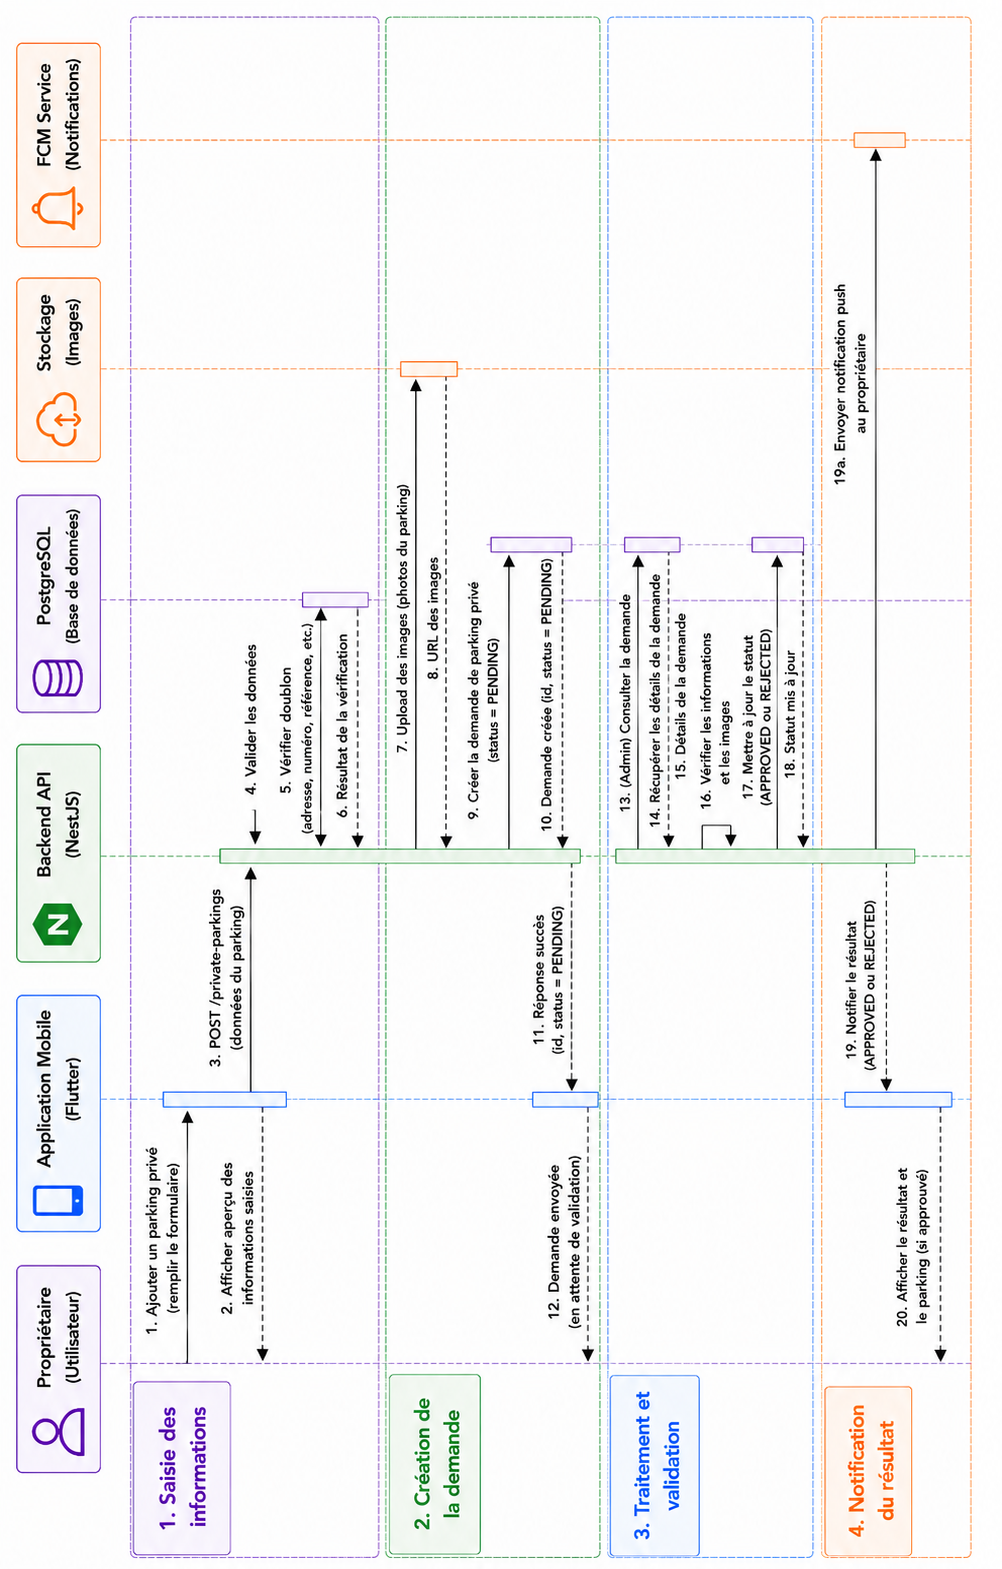
\includegraphics[width=\textwidth]{img/ajout_parking.png}
    \caption{Ajout d'un parking privé}
    \label{fig:sequence_private_parking}
\end{figure}


\subsection{Diagramme de séquence des notifications}

\par Le diagramme de séquence des notifications présente le processus d'envoi d'une notification à un utilisateur de l'application \textbf{TuniPark}. Lorsqu'un événement important se produit, tel que la validation d'un parking privé, la confirmation d'un paiement ou l'activation d'une session de stationnement, le Backend crée une notification et le sauvegarde dans la base de données.

\par Il récupère ensuite les jetons FCM associés à l'utilisateur concerné et transmet le contenu de la notification à \textbf{Firebase Cloud Messaging} \cite{firebase}. Ce service se charge de l'envoyer vers l'appareil mobile de l'utilisateur. La notification reste également disponible dans l'application afin de pouvoir être consultée ultérieurement et marquée comme lue.

\begin{figure}[H]
    \centering
    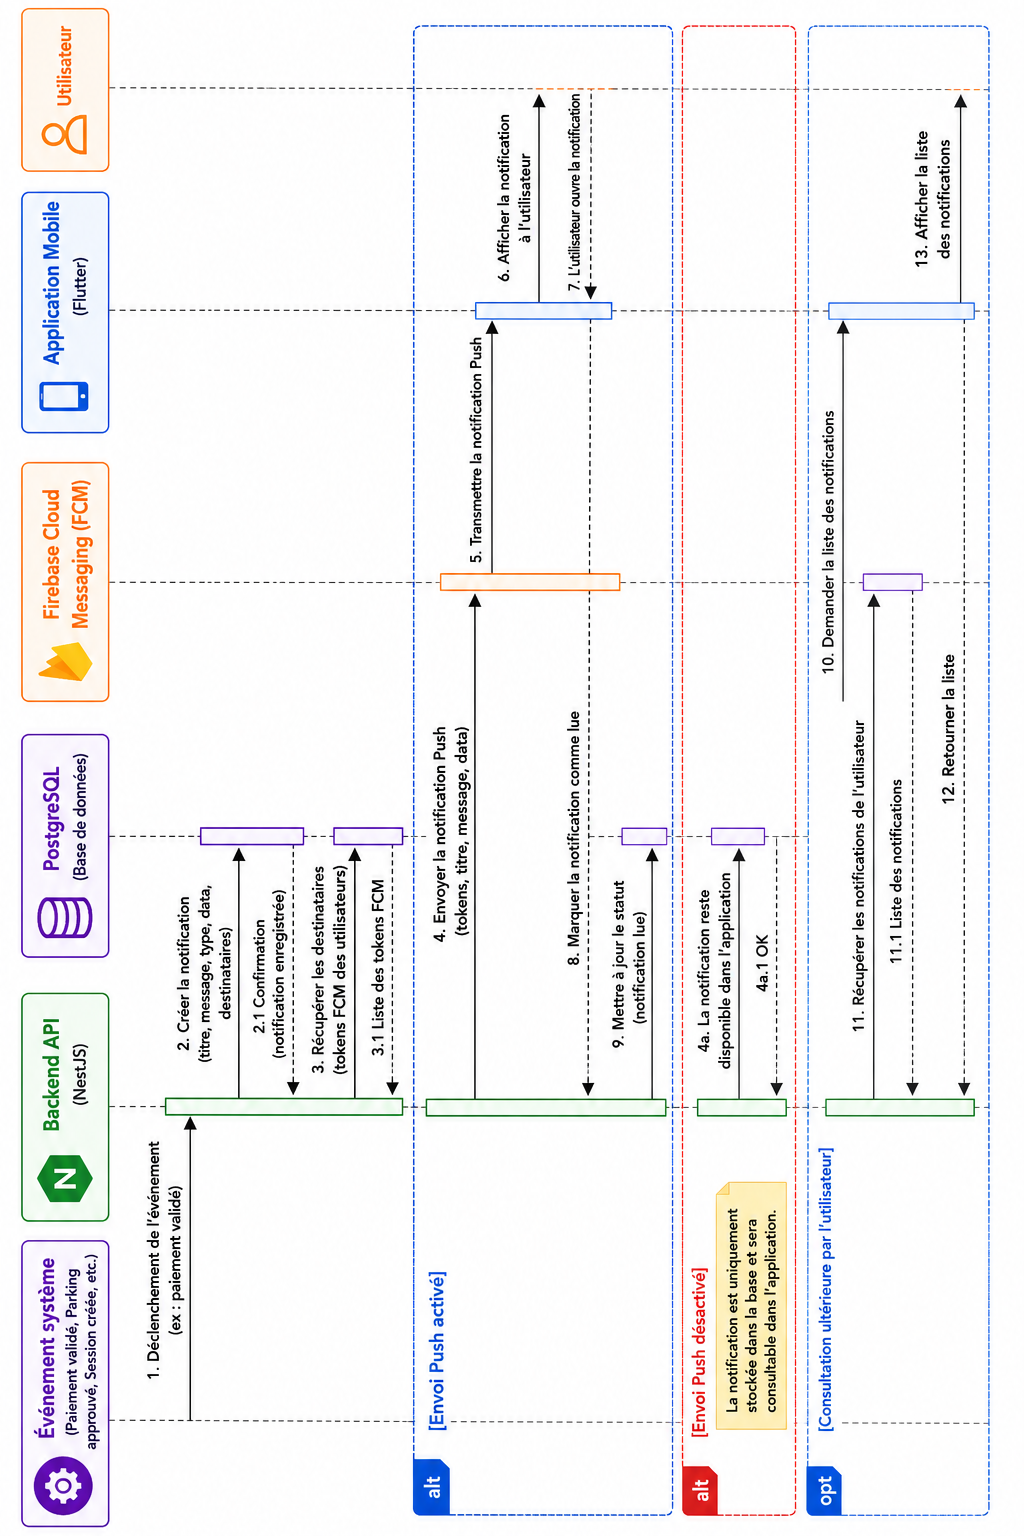
\includegraphics[width=0.95\textwidth]{img/seq_notifications.png}
    \caption{Envoi des notifications}
    \label{fig:sequence_notifications}
\end{figure}

\section{Conclusion}

\par Ce chapitre a présenté la conception et l'architecture de l'application \textbf{TuniPark}. Il a décrit les architectures logique et physique du système, puis les principaux choix techniques retenus pour le développement des différents composants de la solution.

\par Le chapitre a également présenté la conception de la base de données ainsi que les principaux modèles UML utilisés pour représenter le fonctionnement de l'application. Le diagramme de classes a mis en évidence les principales entités du système et leurs relations, Alors que les diagrammes de séquence ont dépeint le déroulement des processus principaux, notamment l'authentification des utilisateurs, la création et le paiement d'une session de stationnement, la recommandation intelligente des parkings, l'ajout d'un parking privé ainsi que l'envoi des notifications.

\par L'ensemble de ces éléments de conception constitue une base robuste pour la phase d'implémentation de l'application. Le chapitre suivant abordera à l'implémentation de TuniPark et présentera les différents modules développés, les interfaces utilisateur ainsi que les principales fonctionnalités mises en œuvre.
\chapter{Réalisation et Implémentation}
\label{chap:implementation}

\section{Introduction}

\par Après avoir présenté l'analyse des besoins ainsi que la conception de l'application TuniPark, ce chapitre décrit la phase de réalisation du projet. Il présente les principaux outils utilisés durant le développement ainsi que l'implémentation des différents modules constituant la solution.

\par Le chapitre présente tout d'abord l'environnement de développement adopté, puis décrit l'implémentation du Backend, de l'application mobile Flutter, de la plateforme web d'administration Angular, ainsi que l'intégration des différents services externes. Enfin, il présente le système de recommandation intelligent ainsi que les principales fonctionnalités développées.


\section{Environnement de développement}

\par La réalisation de l'application \textbf{TuniPark} a nécessité l'utilisation de plusieurs outils et technologies couvrant le développement mobile, le développement web, le développement Backend, l'IA, la gestion de la base de données, les tests, le déploiement tout comme l'intégration de différents services externes. Ces technologies ont été sélectionnées afin de garantir une architecture moderne, performante et facilement maintenable.

\begin{table}[H]
\centering
\small
\renewcommand{\arraystretch}{1.25}
\begin{tabular}{|p{0.32\textwidth}|p{0.58\textwidth}|}
\hline
\textbf{Outil / Technologie} & \textbf{Mise en œuvre dans le projet} \\
\hline
\textbf{Flutter} & Réalisation de l'application mobile destinée aux utilisateurs. \\
\hline
\textbf{Angular} & Élaboration de la plateforme en ligne d'administration. \\
\hline
\textbf{NestJS} & Développement de l'API Backend et de la logique métier. \\
\hline
\textbf{Prisma ORM} & Couche d'accès aux données et gestion des modèles PostgreSQL. \\
\hline
\textbf{PostgreSQL} & Stockage des données de l'application (utilisateurs, parkings, sessions, paiements, notifications, etc.). \\
\hline
\textbf{Python FastAPI} & Développement du microservice d'IA utilisé pour la recommandation des parkings. \\
\hline
\textbf{Scikit-learn (Random Forest)} & Implémentation du modèle de recommandation intelligent. \\
\hline
\textbf{Cloudinary} & Stockage et gestion des images des parkings. \\
\hline
\textbf{Firebase Cloud Messaging} & Envoi des notifications Push vers les appareils mobiles. \\
\hline
\textbf{Flouci} & Gestion des paiements électroniques des sessions de stationnement. \\
\hline
\textbf{Nodemailer} & Envoi des courriers électroniques (vérification et récupération de compte). \\
\hline
\textbf{Twilio} & Gestion des codes OTP par SMS (prévu, non activé durant le projet). \\
\hline
\textbf{Postman} & Test et validation des services REST du Backend. \\
\hline
\textbf{Render} & Plateforme utilisée pour héberger le Backend NestJS, le microservice IA basé sur FastAPI, ainsi que la base de données PostgreSQL. \\
\hline
\textbf{Vercel} & Hébergement de la plateforme web d'administration Angular. \\
\hline
\textbf{Git \& GitHub} & Gestion des versions et collaboration durant le développement. \\
\hline
\end{tabular}
\caption{Principaux outils et technologies utilisés lors de l'implémentation de TuniPark}
\label{tab:implementation_tools}
\end{table}
\section{Implémentation du Backend}

\par Le Backend de \textbf{TuniPark} a été développé à l'aide du framework \textbf{NestJS}. Il constitue le cœur de l'application en assurant le traitement des requêtes provenant de l'application mobile Flutter et de la plateforme web d'administration Angular. Il applique les règles métier, communique avec la base de données PostgreSQL via Prisma ORM et interagit avec plusieurs services externes tels que Flouci, Firebase Cloud Messaging, Cloudinary, Nodemailer ainsi que le microservice d'IA.

\par Afin de garantir une architecture claire, évolutive et facilement maintenable, le Backend est organisé suivant une architecture modulaire. Chaque module est responsable d'un domaine fonctionnel spécifique, ce qui facilite le développement, les tests unitaires et l'évolution future de l'application.
\subsection{Module d'authentification}

\par Le module d'authentification assure la sécurisation de l'accès à l'application. Il prend en charge l'inscription, la connexion, le renouvellement des sessions ainsi que la récupération de mot de passe.

\par Suite à une authentification réussie, le Backend produit un jeton d'accès et un jeton de renouvellement basés sur JWT. Les accès aux différentes fonctionnalités sont ensuite contrôlés en fonction du rôle de l'utilisateur (\textit{Utilisateur}, \textit{Administrateur}, \textit{Propriétaire de parking} ou \textit{Auditeur}). Le module intègre également la vérification des adresses électroniques via Nodemailer ainsi que la vérification des numéros de téléphone par code OTP.

\begin{figure}[H]
    \centering
    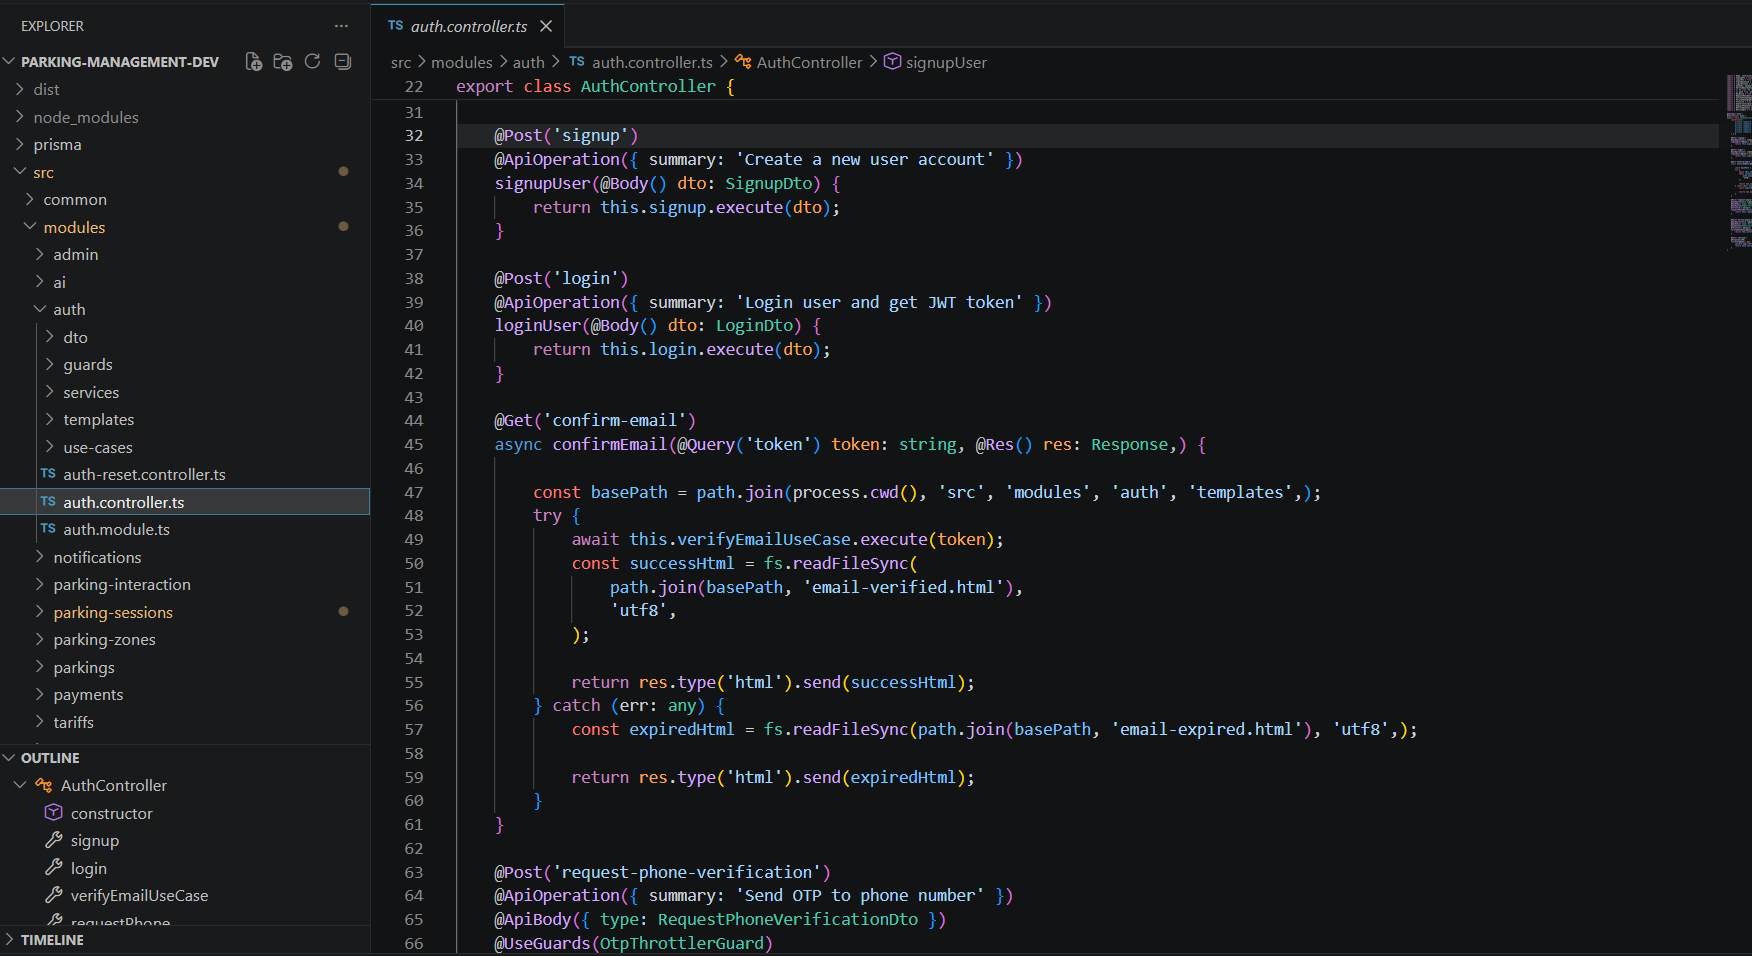
\includegraphics[width=\textwidth]{img/backend_auth.png}
    \caption{Implémentation du module d'authentification}
    \label{fig:backend_auth}
\end{figure}
\subsection{Module de gestion des parkings}

\par Ce module permet la création, la modification et la gestion des parkings publics et privés. Les propriétaires peuvent publier un nouveau parking en renseignant ses caractéristiques, sa localisation, sa capacité, ses horaires, son tarif ainsi que les images correspondantes.

\par Les images sont automatiquement téléversées sur Cloudinary tandis que les informations descriptives sont enregistrées dans PostgreSQL. Les parkings privés sont initialement enregistrés avec le statut \texttt{PENDING} avant d'être validés ou rejetés par un administrateur.

\begin{figure}[H]
    \centering
    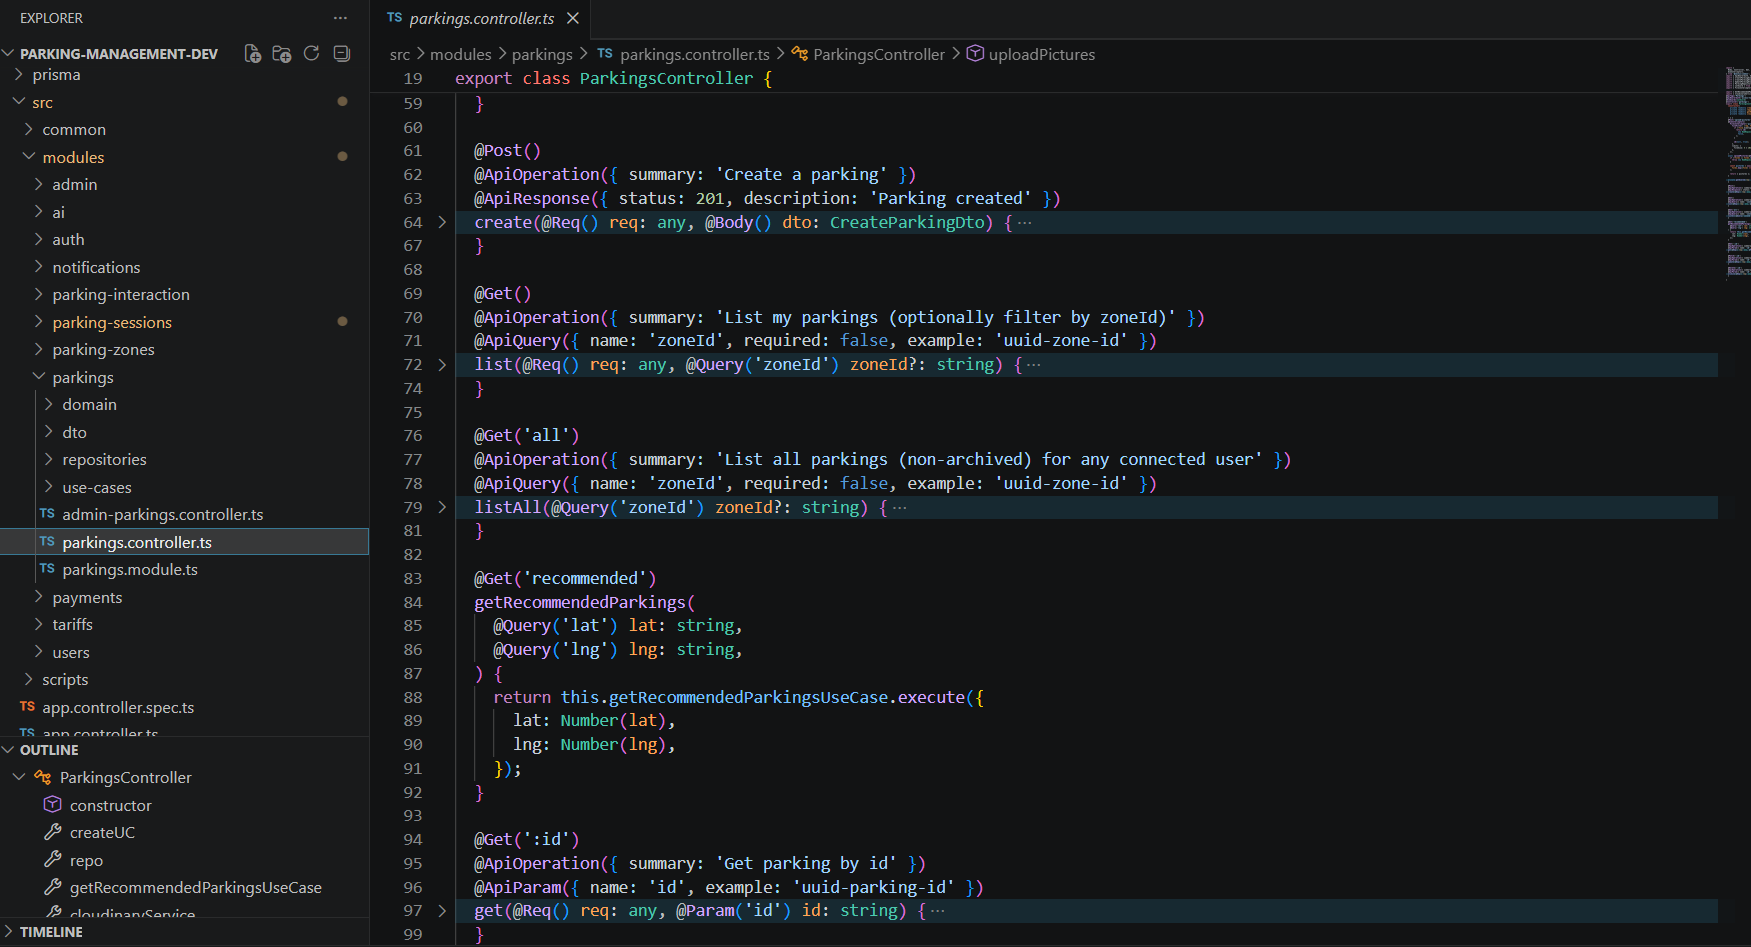
\includegraphics[width=\textwidth]{img/backend_parking.png}
    \caption{Implémentation du module de gestion des parkings}
    \label{fig:backend_parking}
\end{figure}

\subsection{Module de gestion des tarifs}

\par Le module de gestion des tarifs permet d'associer une grille tarifaire à chaque parking. Il prend en charge les différents modes de facturation proposés par la plateforme, notamment le tarif à l'unité, le tarif journalier et le tarif mensuel.

\par Les administrateurs et les propriétaires de parkings peuvent définir ou modifier les tarifs en fonction des caractéristiques de chaque parking. Ces informations sont utilisées lors de la création des sessions de stationnement afin de calculer le montant à payer par l'utilisateur.

\begin{figure}[H]
    \centering
    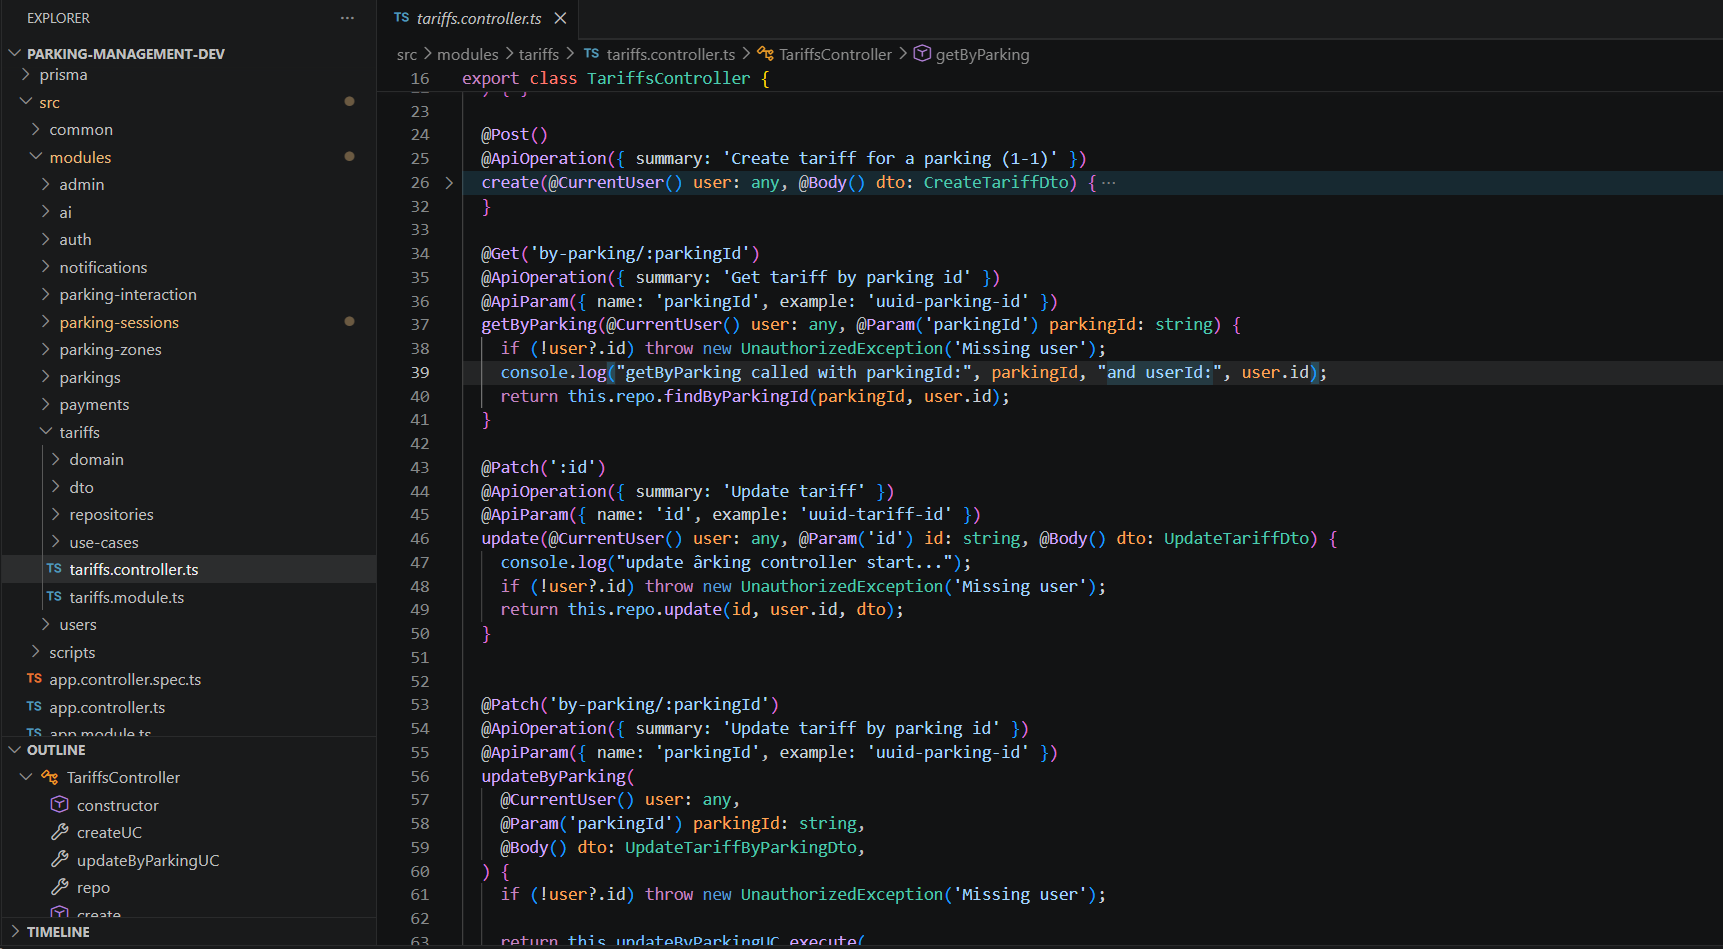
\includegraphics[width=\textwidth]{img/backend_tariff.png}
    \caption{Implémentation du module de gestion des tarifs}
    \label{fig:backend_tariff}
\end{figure}

\subsection{Module de gestion des sessions de stationnement}

\par Le module des sessions permet aux utilisateurs de démarrer, prolonger et terminer une session de stationnement. Lorsqu'un utilisateur sélectionne un parking, le Backend vérifie sa disponibilité avant de créer une nouvelle session avec le statut \texttt{CREATED}.

\par Après validation du paiement, le statut de la session devient \texttt{ACTIVE}. Le module assure également le suivi des différentes étapes du stationnement jusqu'à la fermeture de la session, tout en conservant l'historique des opérations.

\begin{figure}[H]
    \centering
    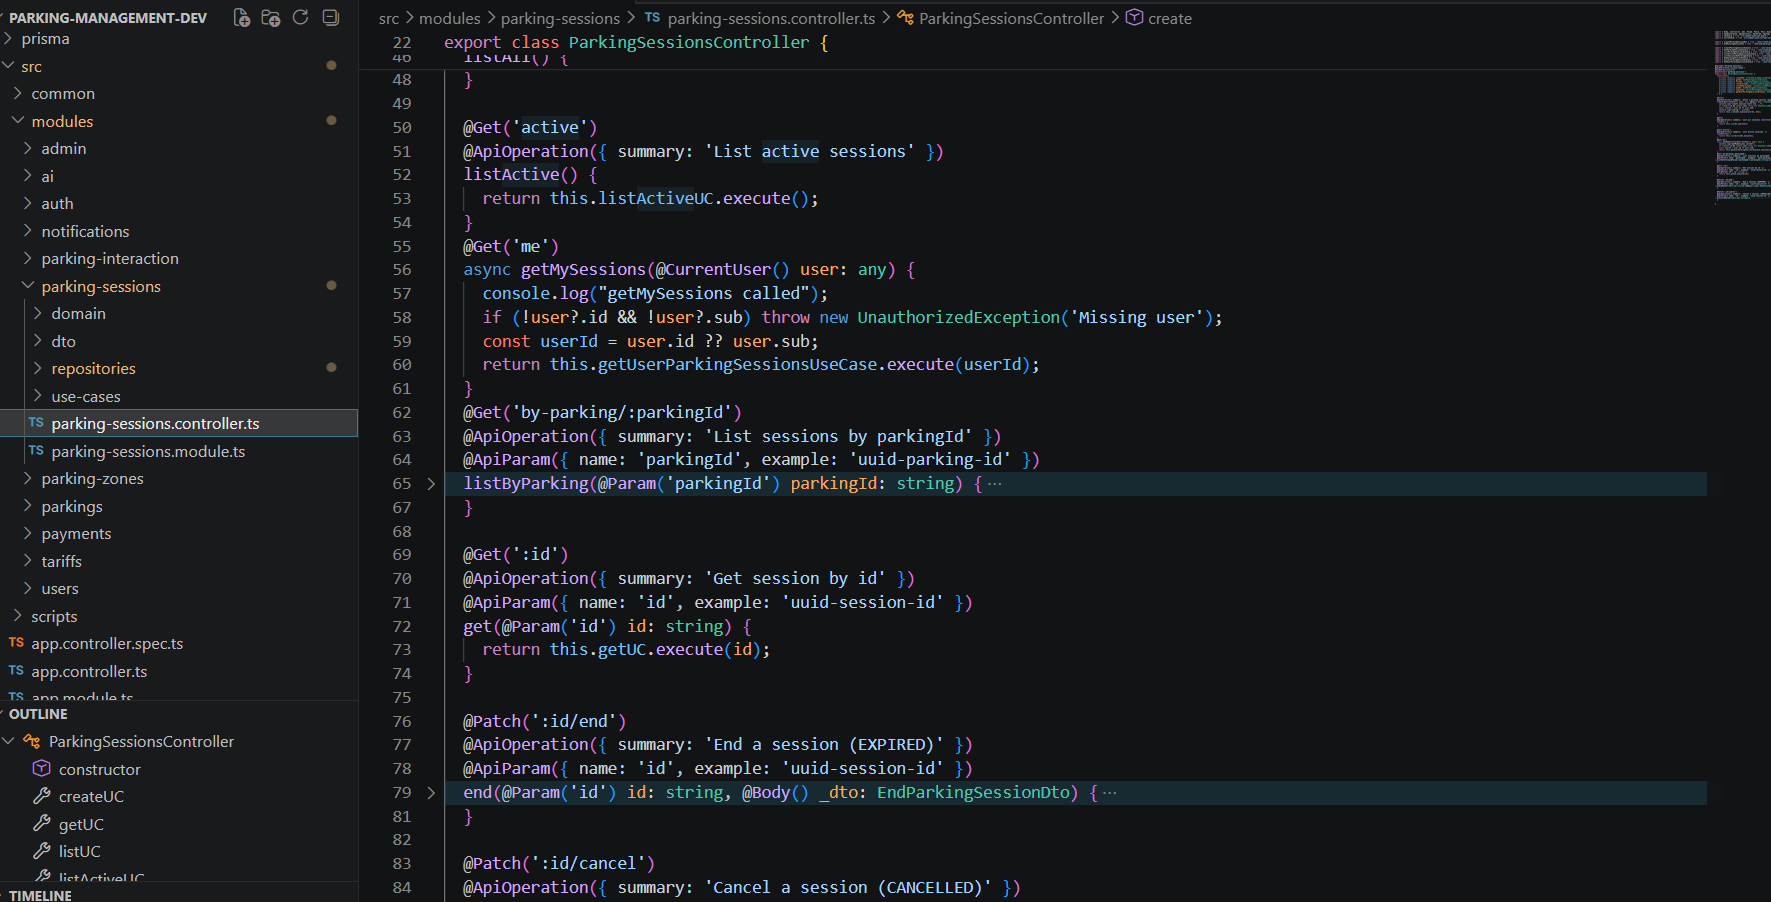
\includegraphics[width=\textwidth]{img/backend_session.png}
    \caption{Implémentation du module des sessions de stationnement}
    \label{fig:backend_session}
\end{figure}

\subsection{Module de paiement}

\par Le module de paiement permet de gérer les transactions financières liées aux sessions de stationnement. Après la création d'une session, le Backend prépare automatiquement la transaction puis redirige l'utilisateur vers la plateforme de paiement \textbf{Flouci}.

\par Une fois le paiement confirmé, Flouci informe le Backend du résultat de la transaction. Celui-ci met alors à jour les informations de paiement ainsi que le statut de la session. Toutes les transactions sont enregistrées dans la base de données afin d'assurer leur traçabilité.

\begin{figure}[H]
    \centering
    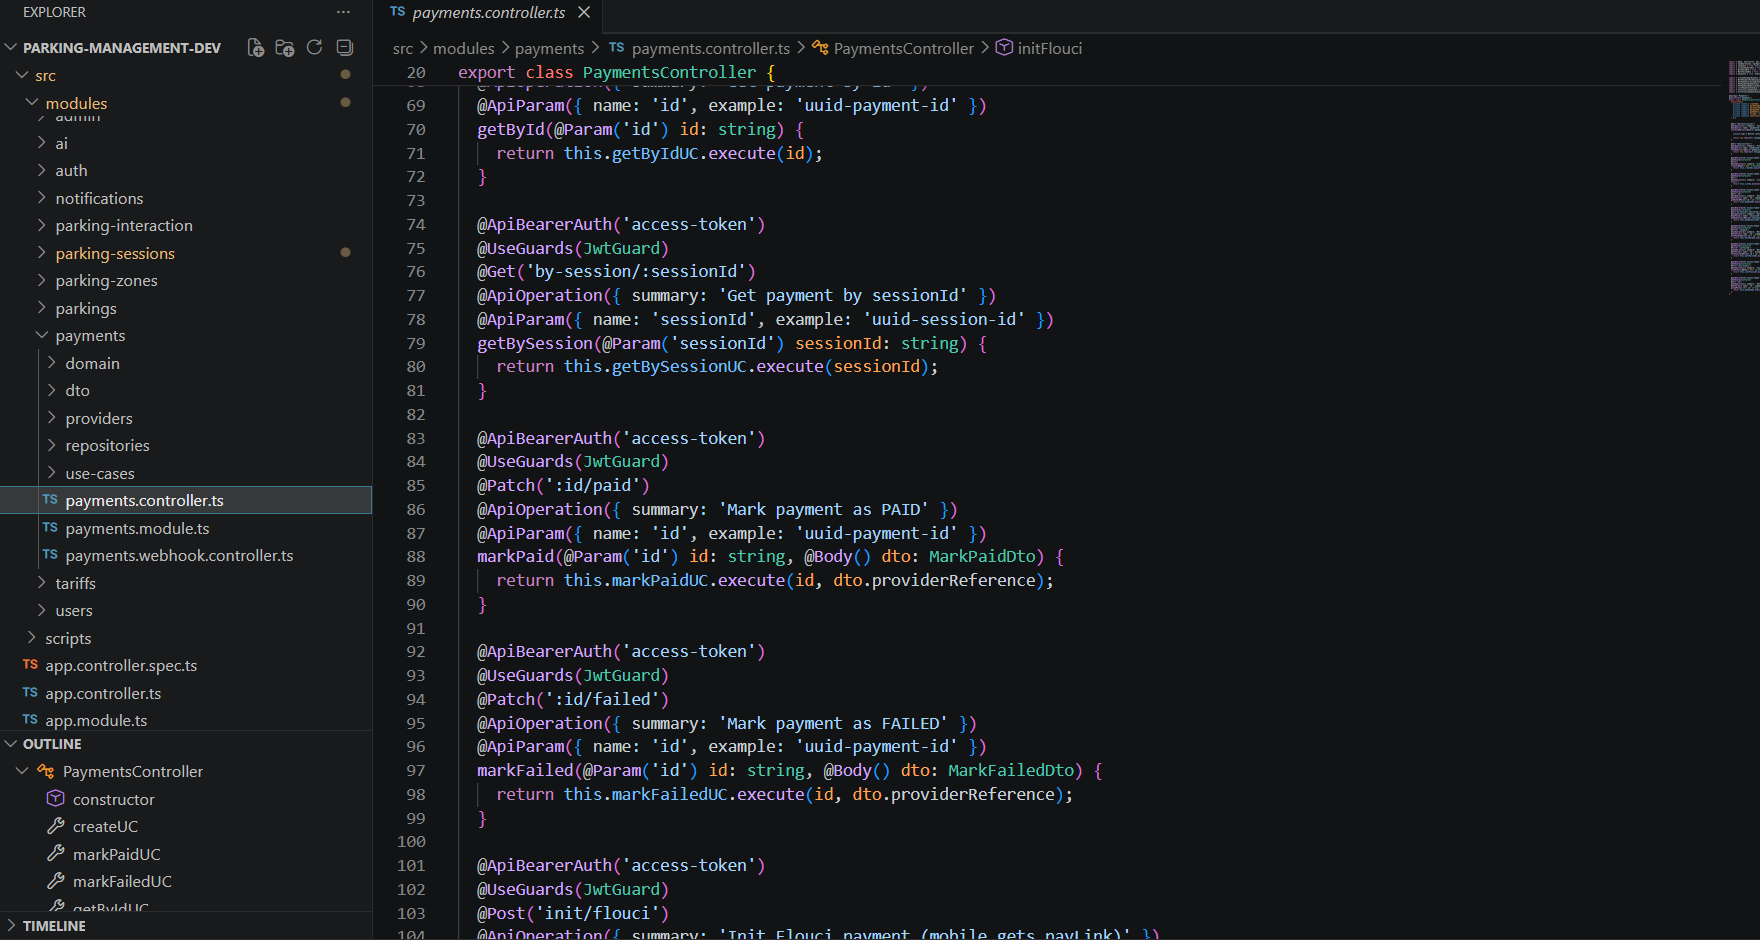
\includegraphics[width=\textwidth]{img/backend_payment.png}
    \caption{Implémentation du module de paiement}
    \label{fig:backend_payment}
\end{figure}
\subsection{Module de recommandation intelligente}

\par Pour offrir une meilleure expérience aux utilisateurs, TuniPark intègre un système de recommandation basé sur l'IA. Le Backend collecte différentes informations relatives aux parkings, notamment leur distance, leur disponibilité, leur tarif ainsi que les statistiques d'utilisation.

\par Ces informations sont transmises à un microservice développé avec \textbf{FastAPI} utilisant un modèle \textbf{Random Forest}. Celui-ci calcule un score de recommandation pour chaque parking et retourne les résultats au Backend, qui les trie avant de les envoyer à l'application mobile. En cas d'indisponibilité du microservice, un algorithme de secours implémenté directement dans le Backend permet de garantir la continuité du service.

\begin{figure}[H]
    \centering
    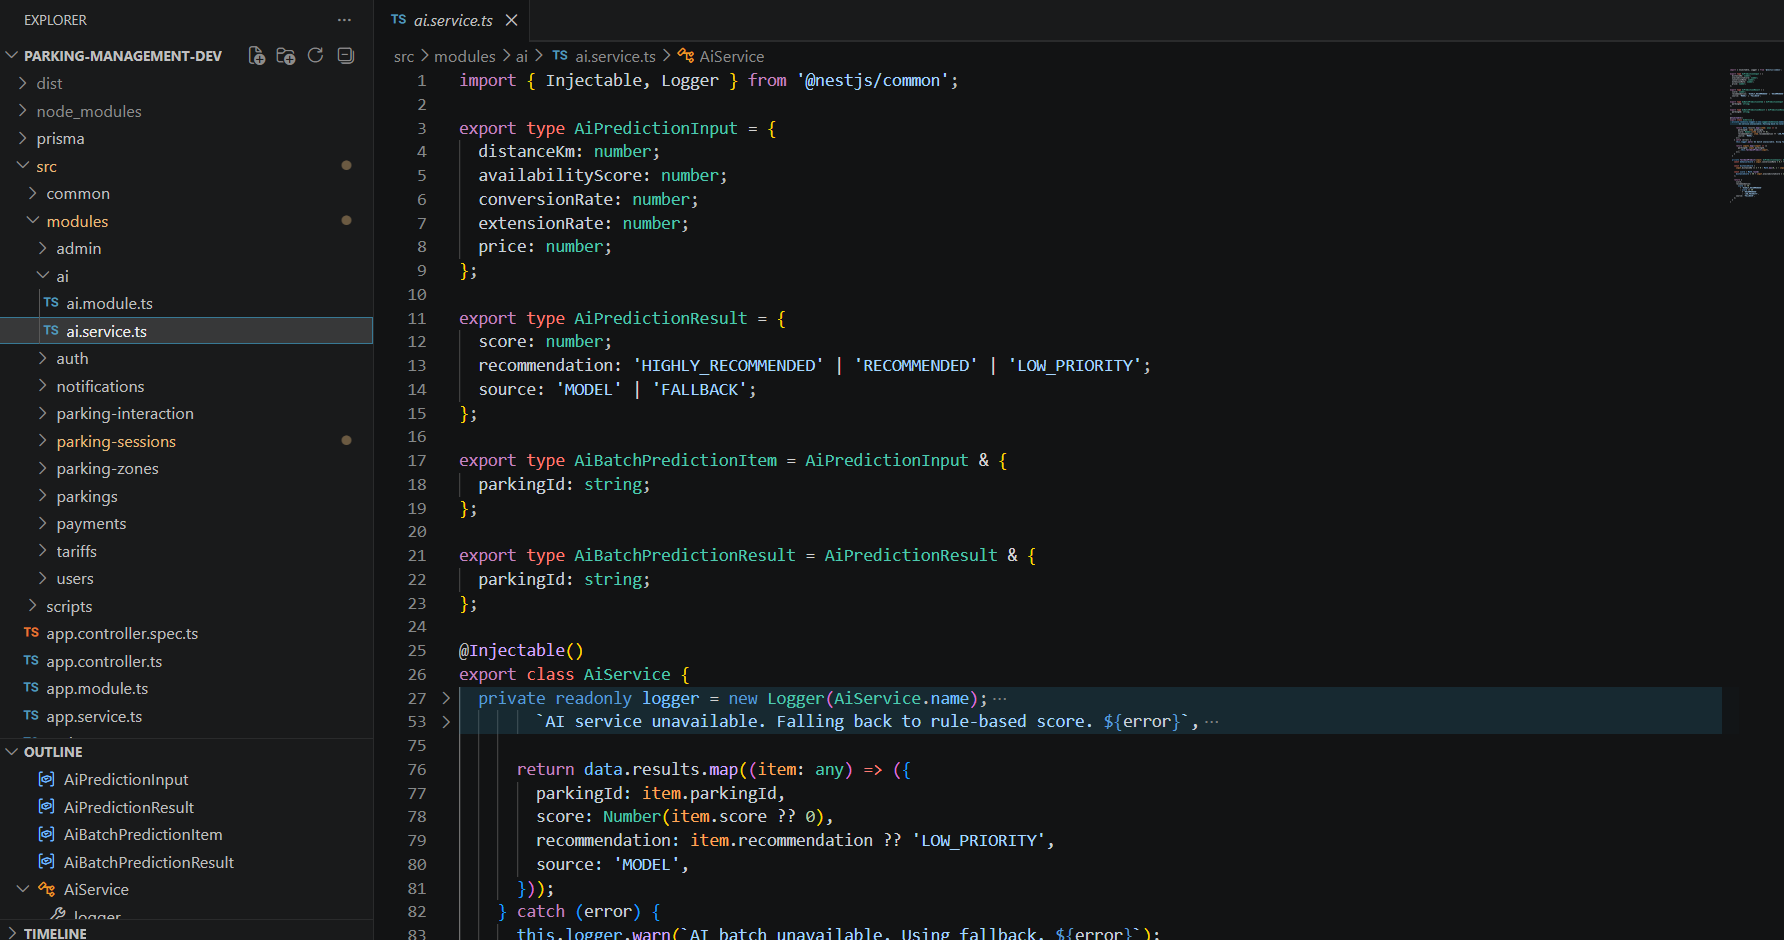
\includegraphics[width=\textwidth]{img/backend_ai.png}
    \caption{Implémentation du module de recommandation intelligente}
    \label{fig:backend_ai}
\end{figure}
\subsection{Module de notifications}

\par Le module de notifications informe les utilisateurs des événements importants de l'application, tels que la validation d'un parking privé, la confirmation d'un paiement ou l'activation d'une session de stationnement.

\par Les notifications sont enregistrées dans la base de données et transmises aux appareils mobiles grâce à \textbf{Firebase Cloud Messaging}. Les jetons FCM des utilisateurs sont également gérés par ce module afin d'assurer la distribution des notifications Push.

\begin{figure}[H]
    \centering
    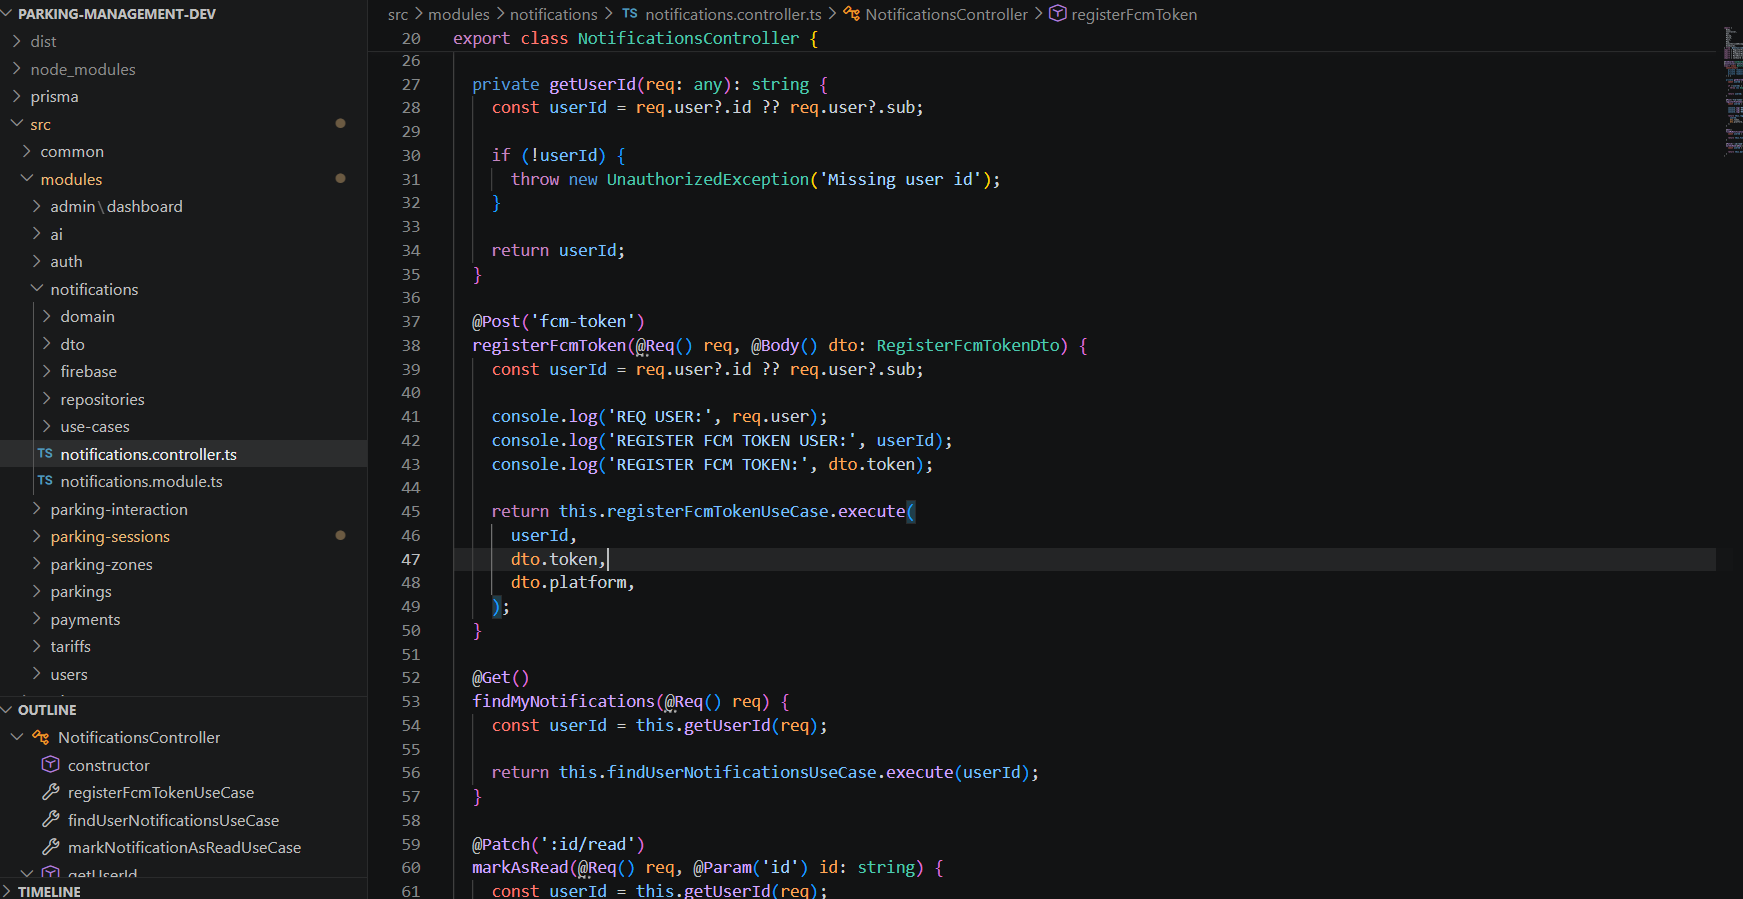
\includegraphics[width=\textwidth]{img/backend_notification.png}
    \caption{Implémentation du module de notifications}
    \label{fig:backend_notification}
\end{figure}

\subsection{Module des interactions avec les parkings}

\par Le module des interactions enregistre les différentes actions réalisées par les utilisateurs sur les parkings. Chaque consultation d'un parking, démarrage de session ou prolongation de stationnement est enregistrée dans la base de données.

\par Ces informations permettent de produire des statistiques d'utilisation et sont exploitées par le système de recommandation intelligent afin d'évaluer la popularité des parkings et d'améliorer la pertinence des recommandations proposées aux utilisateurs.

\begin{figure}[H]
    \centering
    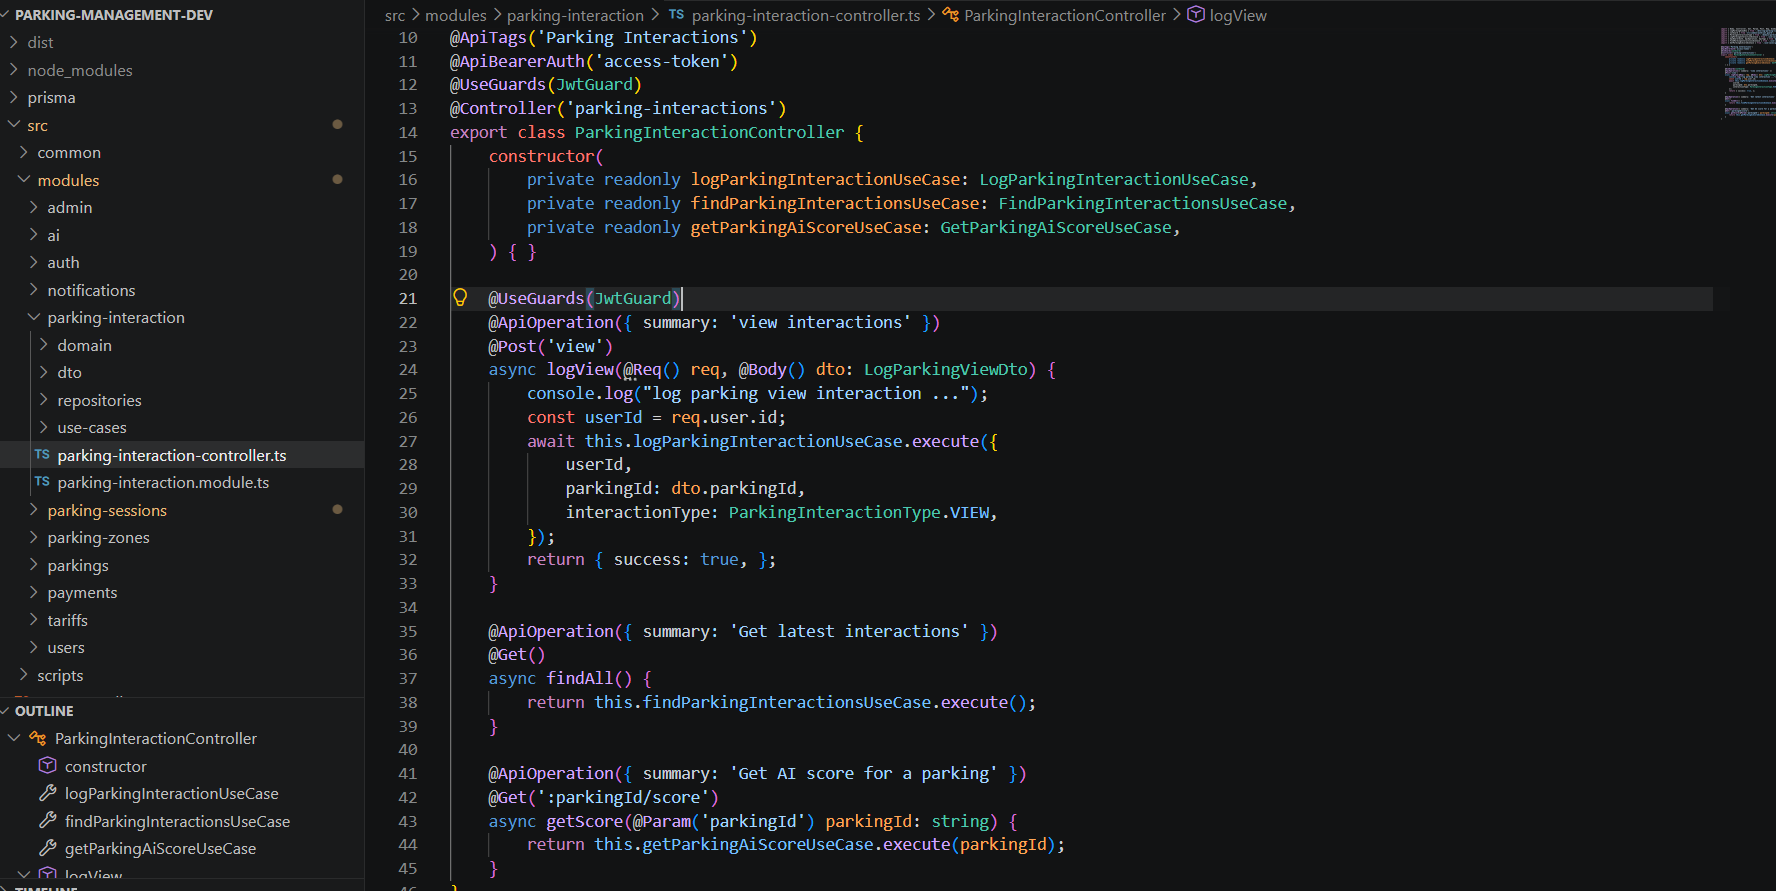
\includegraphics[width=\textwidth]{img/backend_interaction.png}
    \caption{Implémentation du module des interactions avec les parkings}
    \label{fig:backend_interaction}
\end{figure}


\subsection{Module de gestion des utilisateurs}

\par Ce module permet de gérer les comptes des utilisateurs de la plateforme. Il prend en charge la création des comptes, la mise à jour des informations personnelles, la gestion des rôles ainsi que la vérification des adresses électroniques et des numéros de téléphone.

\par Le module assure également l'administration des comptes, notamment le blocage d'un utilisateur, la récupération du mot de passe et la gestion des différents profils tels que les utilisateurs, les propriétaires de parkings, les auditeurs et les administrateurs.

\begin{figure}[H]
    \centering
    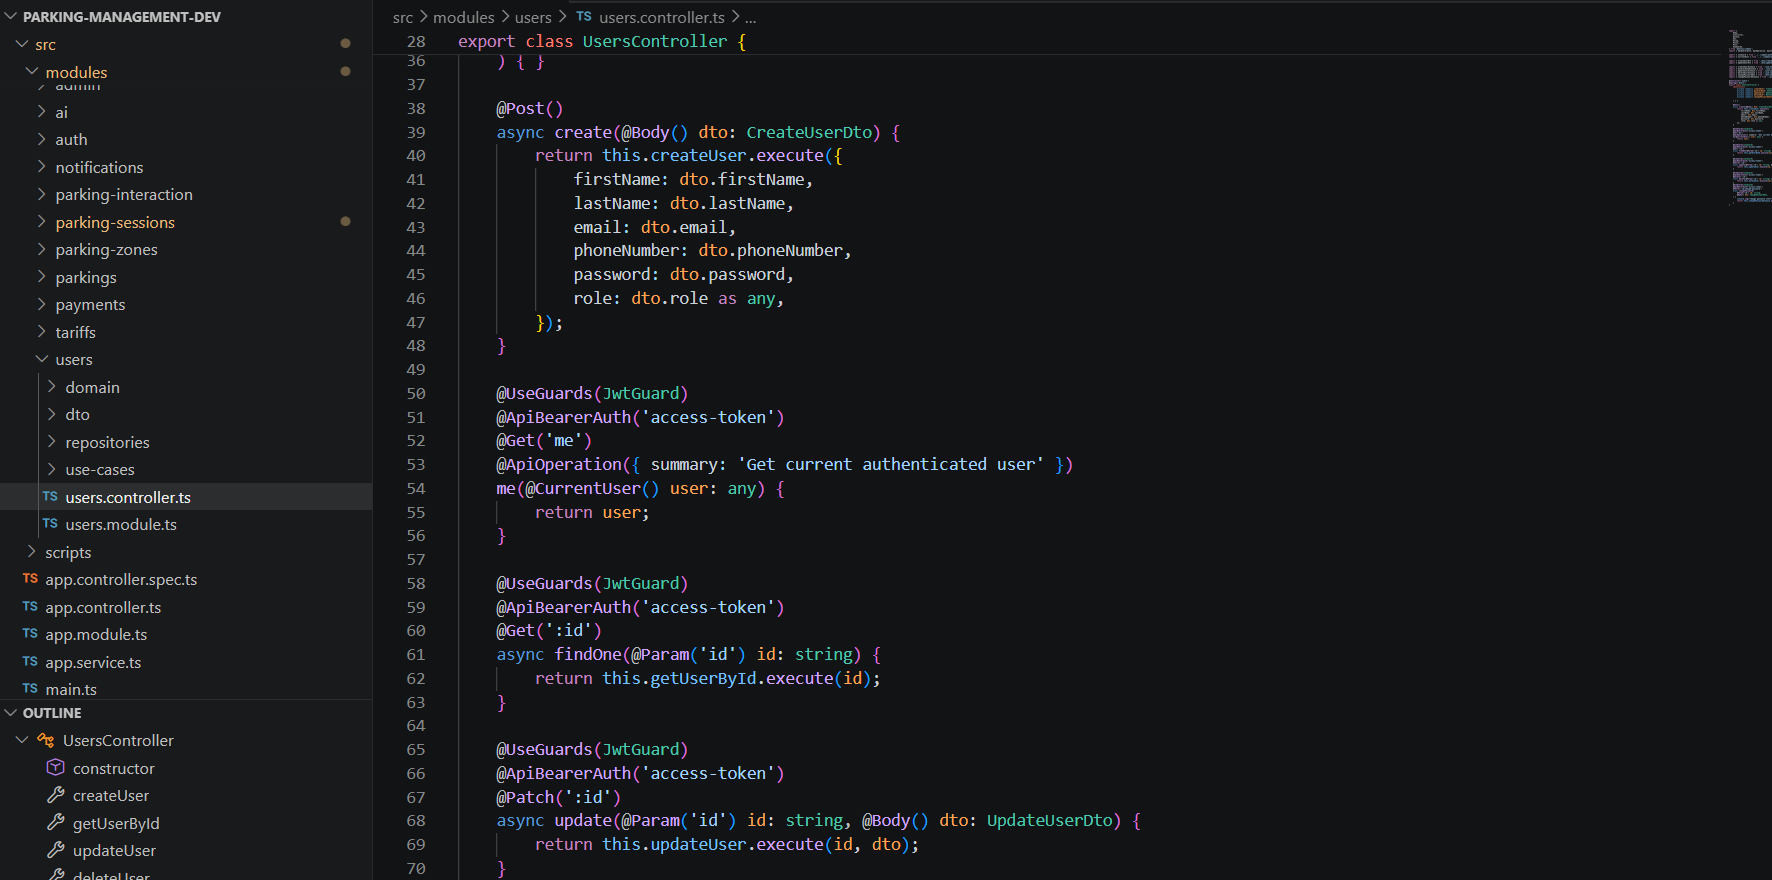
\includegraphics[width=\textwidth]{img/backend_user.png}
    \caption{Implémentation du module de gestion des utilisateurs}
    \label{fig:backend_user}
\end{figure}



\section{Implémentation de l'application mobile}

\par \textbf{TuniPark} a été développée à l'aide du framework \textbf{Flutter}. Elle permet aux utilisateurs de rechercher des parkings, de gérer leurs sessions de stationnement, d'effectuer des paiements sécurisés et de consulter leur historique. L'application adopte une architecture modulaire reposant sur le principe du \textit{Clean Architecture}, ce qui facilite la maintenance, les évolutions futures et la réutilisation du code.

\par Les interfaces ont été conçues afin d'offrir une navigation simple et intuitive tout en exploitant les fonctionnalités natives du smartphone, notamment la géolocalisation, les notifications Push et le stockage sécurisé des informations d'authentification.


\subsection{Authentification}

\par Ces interfaces permettent aux utilisateurs de créer un compte, de se connecter et de récupérer leur mot de passe. La plateforme prend en charge l'authentification par adresse électronique ou numéro de téléphone. En cas d'oubli du mot de passe, un code OTP est envoyé afin de vérifier l'identité de l'utilisateur avant de lui permettre de définir un nouveau mot de passe.

\begin{figure}[H]
    \centering
    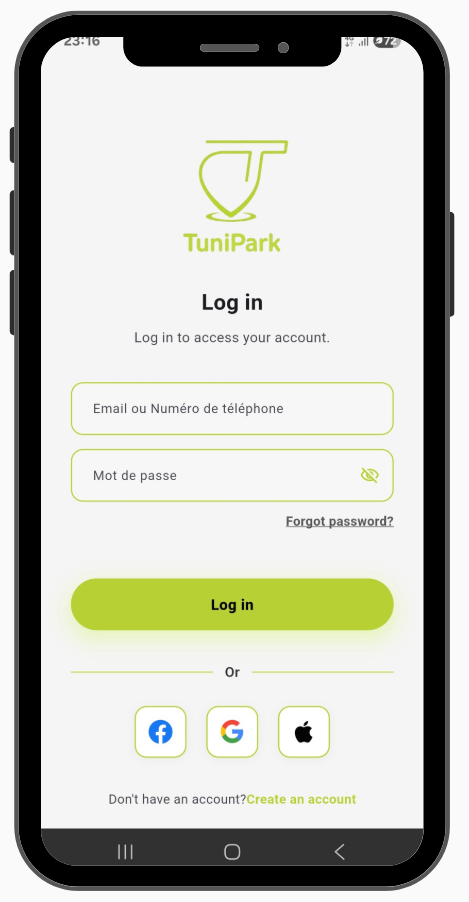
\includegraphics[width=0.5\textwidth]{img/auth_screens.png}
    \caption{Interfaces d'authentification}
    \label{fig:auth_screens}
\end{figure}

\subsection{Exploration des parkings}

\par Après authentification, l'utilisateur accède à la page d'exploration. Celle-ci affiche les parkings disponibles à proximité sous forme de carte interactive accompagnée de recommandations générées par le système intelligent. L'utilisateur a la possibilité de visualiser les détails de chaque parking avant de démarrer une session.

\begin{figure}[H]
    \centering
    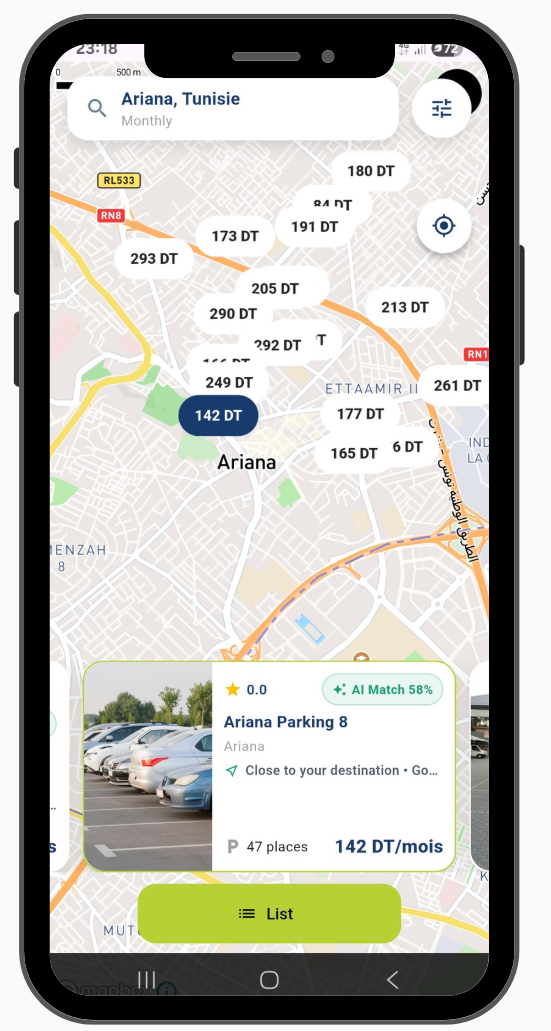
\includegraphics[width=0.5\textwidth]{img/explore_screens.png}
    \caption{Exploration des parkings}
    \label{fig:explore}
\end{figure}

\subsection{Création d'une session de stationnement}

\par Pour démarrer une session de stationnement, l'utilisateur sélectionne un parking puis renseigne les informations nécessaires concernant son véhicule et la durée souhaitée. Une fois les informations validées, l'application lance automatiquement le processus de paiement.

\begin{figure}[H]
    \centering
    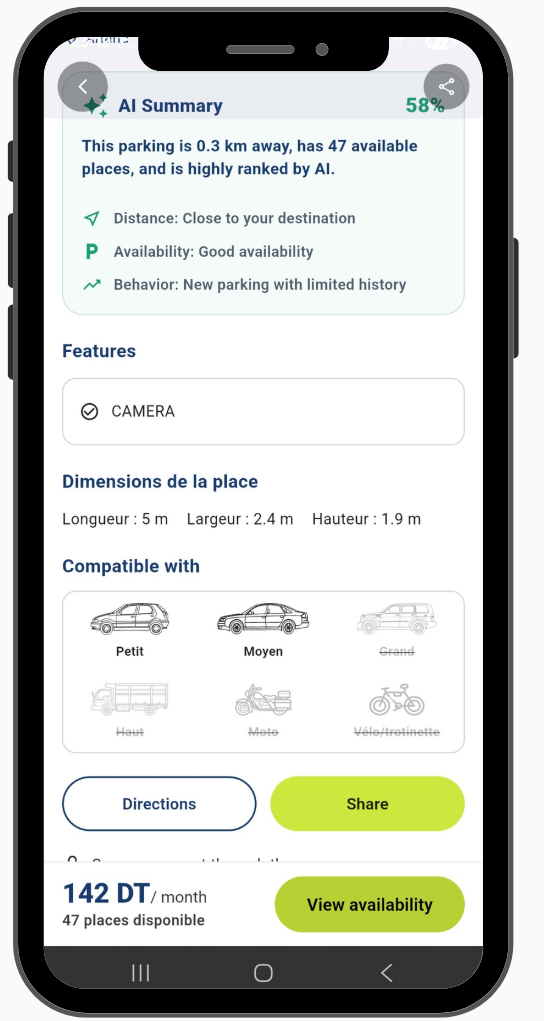
\includegraphics[width=0.5\textwidth]{img/session_creation.png}
    \caption{Création d'une session de stationnement}
    \label{fig:create_session}
\end{figure}

\subsection{Paiement d'une session}

\par Les paiements sont réalisés via la plateforme Flouci. Après validation de la transaction, l'application reçoit la confirmation du Backend et active automatiquement la session de stationnement.

\begin{figure}[H]
    \centering
    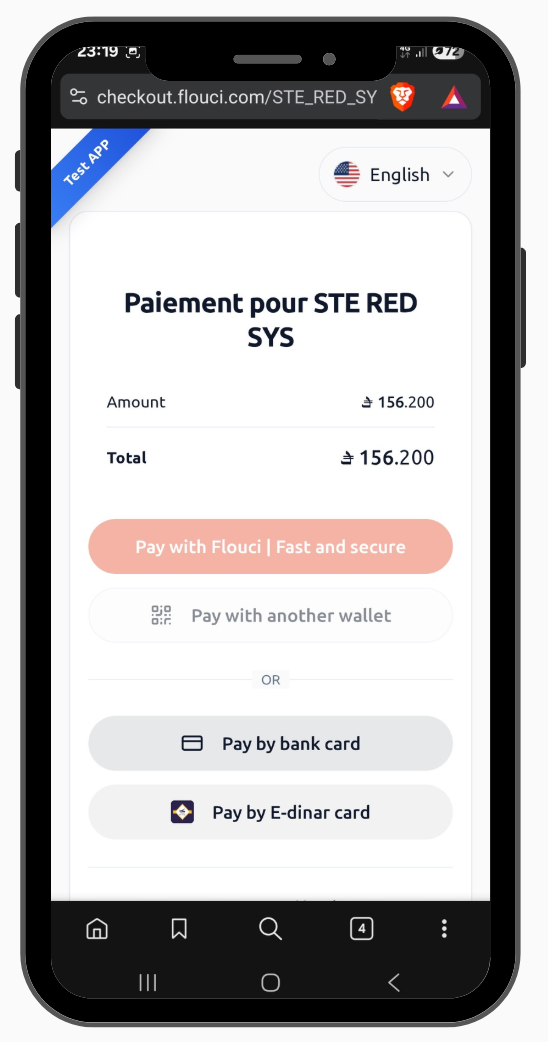
\includegraphics[width=.5\textwidth]{img/payment_screens.png}
    \caption{Paiement d'une session}
    \label{fig:payment}
\end{figure}

\subsection{Suivi de la session}

\par Une fois le paiement confirmé, l'usager a la possibilité de visualiser les détails concernant sa session actuelle, notamment le parking sélectionné, la durée restante et les différentes actions disponibles telles que la prolongation ou l'arrêt de la session.

\begin{figure}[H]
    \centering
    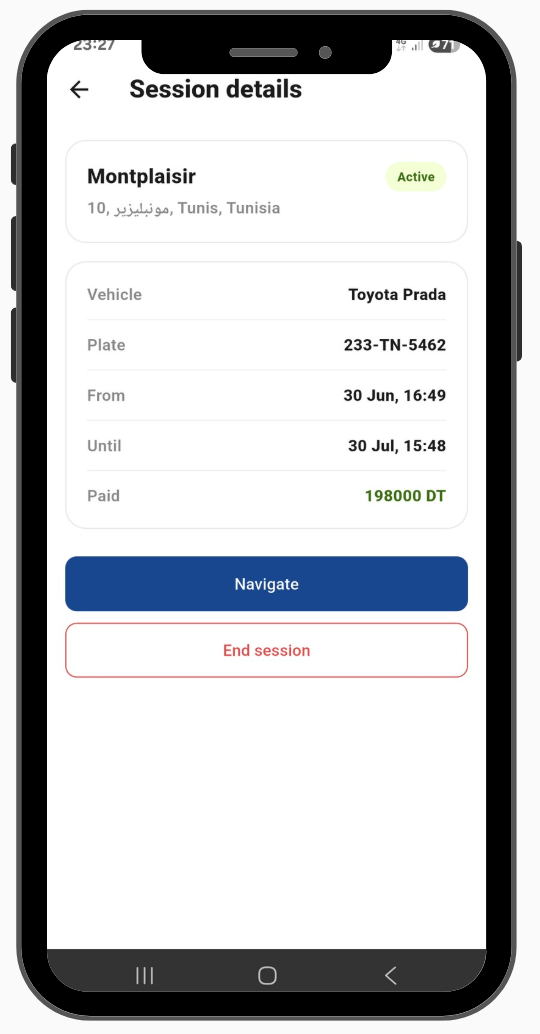
\includegraphics[width=.5\textwidth]{img/session_active.png}
    \caption{Suivi d'une session active}
    \label{fig:active_session}
\end{figure}

\subsection{Ajout d'un parking privé}

\par Les propriétaires peuvent proposer un parking privé en renseignant les informations générales, les caractéristiques, les tarifs et les photographies du parking. Après soumission, la demande est transmise à l'administrateur pour validation.

\begin{figure}[H]
    \centering
    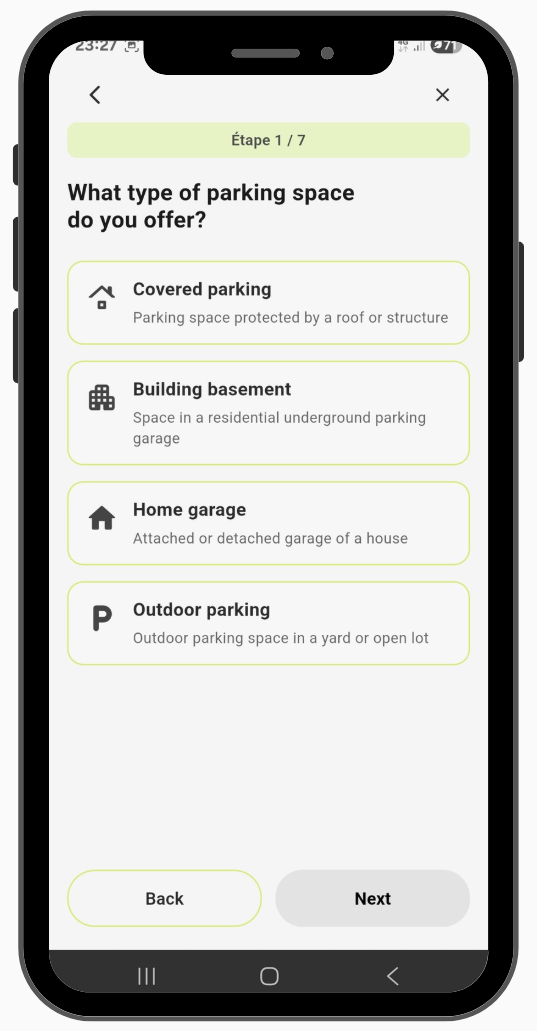
\includegraphics[width=.5\textwidth]{img/private_parking.png}
    \caption{Ajout d'un parking privé}
    \label{fig:private_parking}
\end{figure}
\subsection{Profil utilisateur}

\par L'application permet aux utilisateurs de consulter et de modifier leurs informations personnelles, de gérer leurs véhicules enregistrés ainsi que d'accéder à leur historique de stationnement.

\begin{figure}[H]
    \centering
    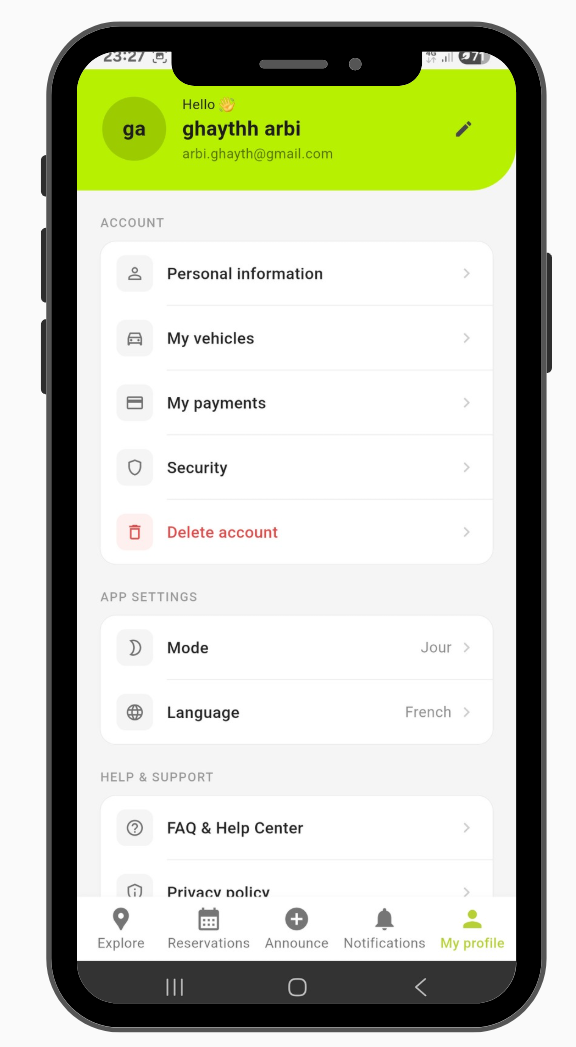
\includegraphics[width=.5\textwidth]{img/profile.png}
    \caption{Interface du profil utilisateur}
    \label{fig:profile}
\end{figure}

\subsection{Notifications}

\par Les notifications permettent d'informer l'utilisateur des événements importants de l'application, notamment la validation d'un parking privé, la confirmation d'un paiement, le début d'une session ou encore les rappels liés au stationnement.

\begin{figure}[H]
    \centering
    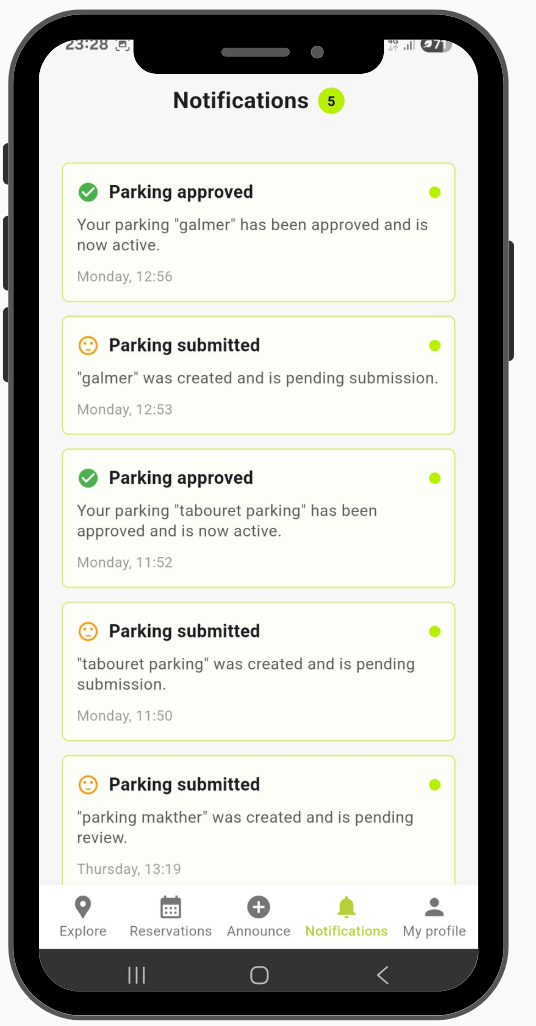
\includegraphics[width=.45\textwidth]{img/notifications.png}
    \caption{Interface des notifications}
    \label{fig:notifications}
\end{figure}
\section{Fonctionnalités administratives}

\par La plateforme web d'administration a été développée avec \textbf{Angular}. Elle est exclusivement accessible aux utilisateurs disposant des privilèges administratifs. Après authentification, l'administrateur accède à un tableau de bord lui permettant de superviser les principales opérations de l'application TuniPark.

\par L'interface d'administration centralise la gestion des utilisateurs, des parkings publics et privés, des zones de stationnement, des sessions, des paiements ainsi que des notifications. Elle permet également de valider ou refuser les requêtes d'ajout de parkings privés, de consulter les statistiques d'utilisation de la plateforme et de gérer les informations nécessaires au bon fonctionnement du système.

\begin{figure}[H]
    \centering
    \begin{minipage}{0.8\textwidth}
        \centering
        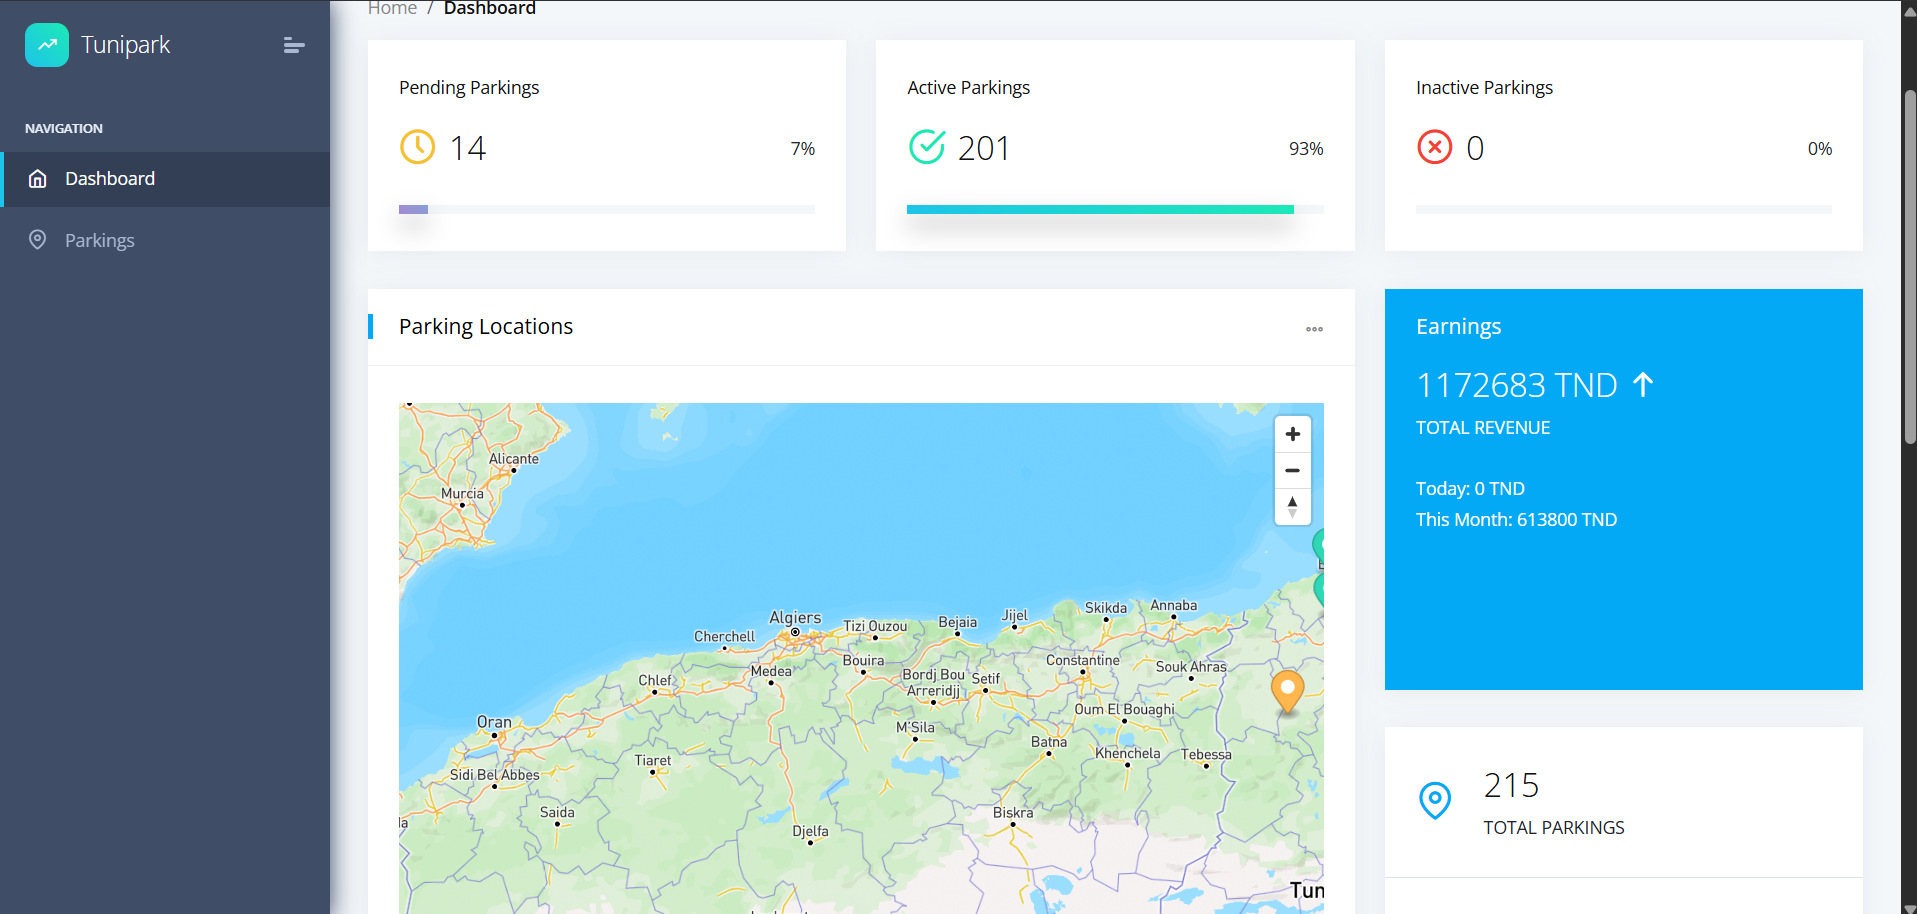
\includegraphics[width=0.95\textwidth]{img/admin_dashboard.png}
        \caption{Tableau de bord de l'administration}
        \label{fig:admin_dashboard}
    \end{minipage}
    \vfill
    \begin{minipage}{0.8\textwidth}
        \centering
        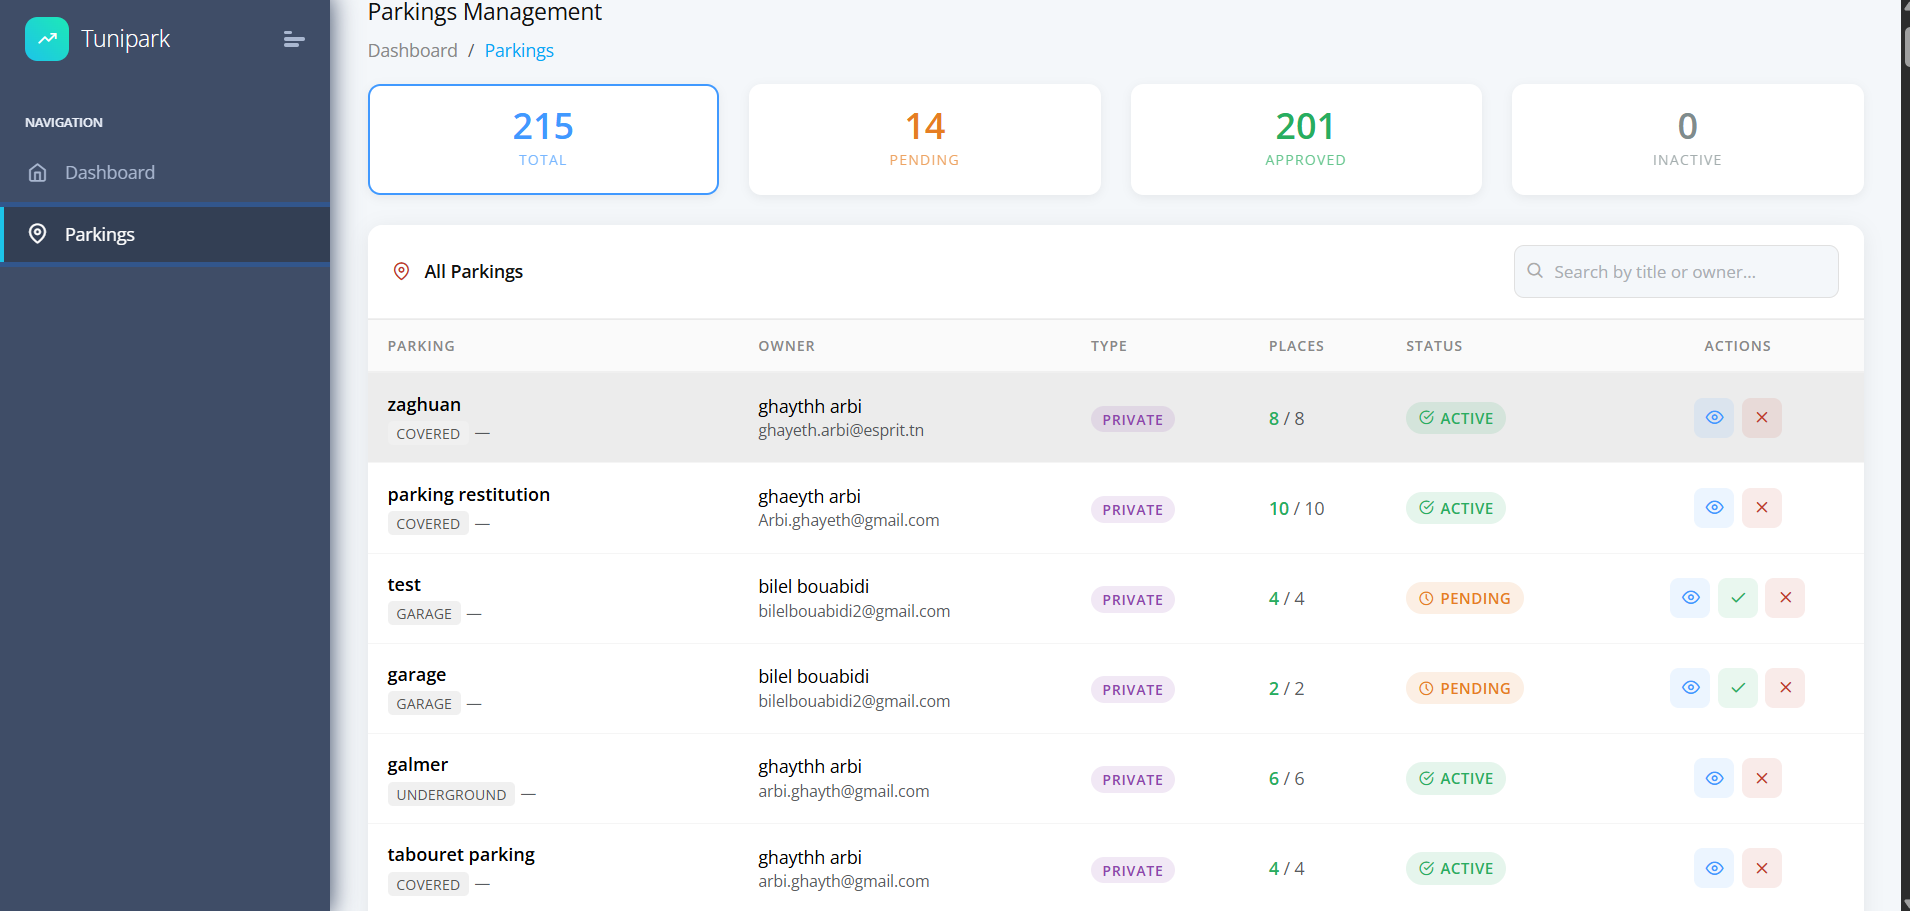
\includegraphics[width=0.95\textwidth]{img/admin_management.png}
        \caption{Interface de gestion des ressources}
        \label{fig:admin_management}
    \end{minipage}
\end{figure}
\section{Présentation du déploiement}

\par Après le développement et la validation des différentes fonctionnalités, l'application \textbf{TuniPark} a été déployée dans un context de production afin de permettre son utilisation dans des conditions réelles. Les différents composants de la plateforme sont hébergés sur des services cloud adaptés à leur rôle, garantissant leur disponibilité, leur maintenance et leur évolutivité.

\par Le Backend développé avec \textbf{NestJS} est hébergé sur la plateforme \textbf{Render}. Cette plateforme assure l'exécution continue de l'API REST ainsi que la communication avec la base de données \textbf{PostgreSQL}, également hébergée sur Render. Cette configuration permet au Backend de traiter les requêtes provenant de l'application mobile et de la plateforme web d'administration de manière sécurisée.

\begin{figure}[H]
    \centering
    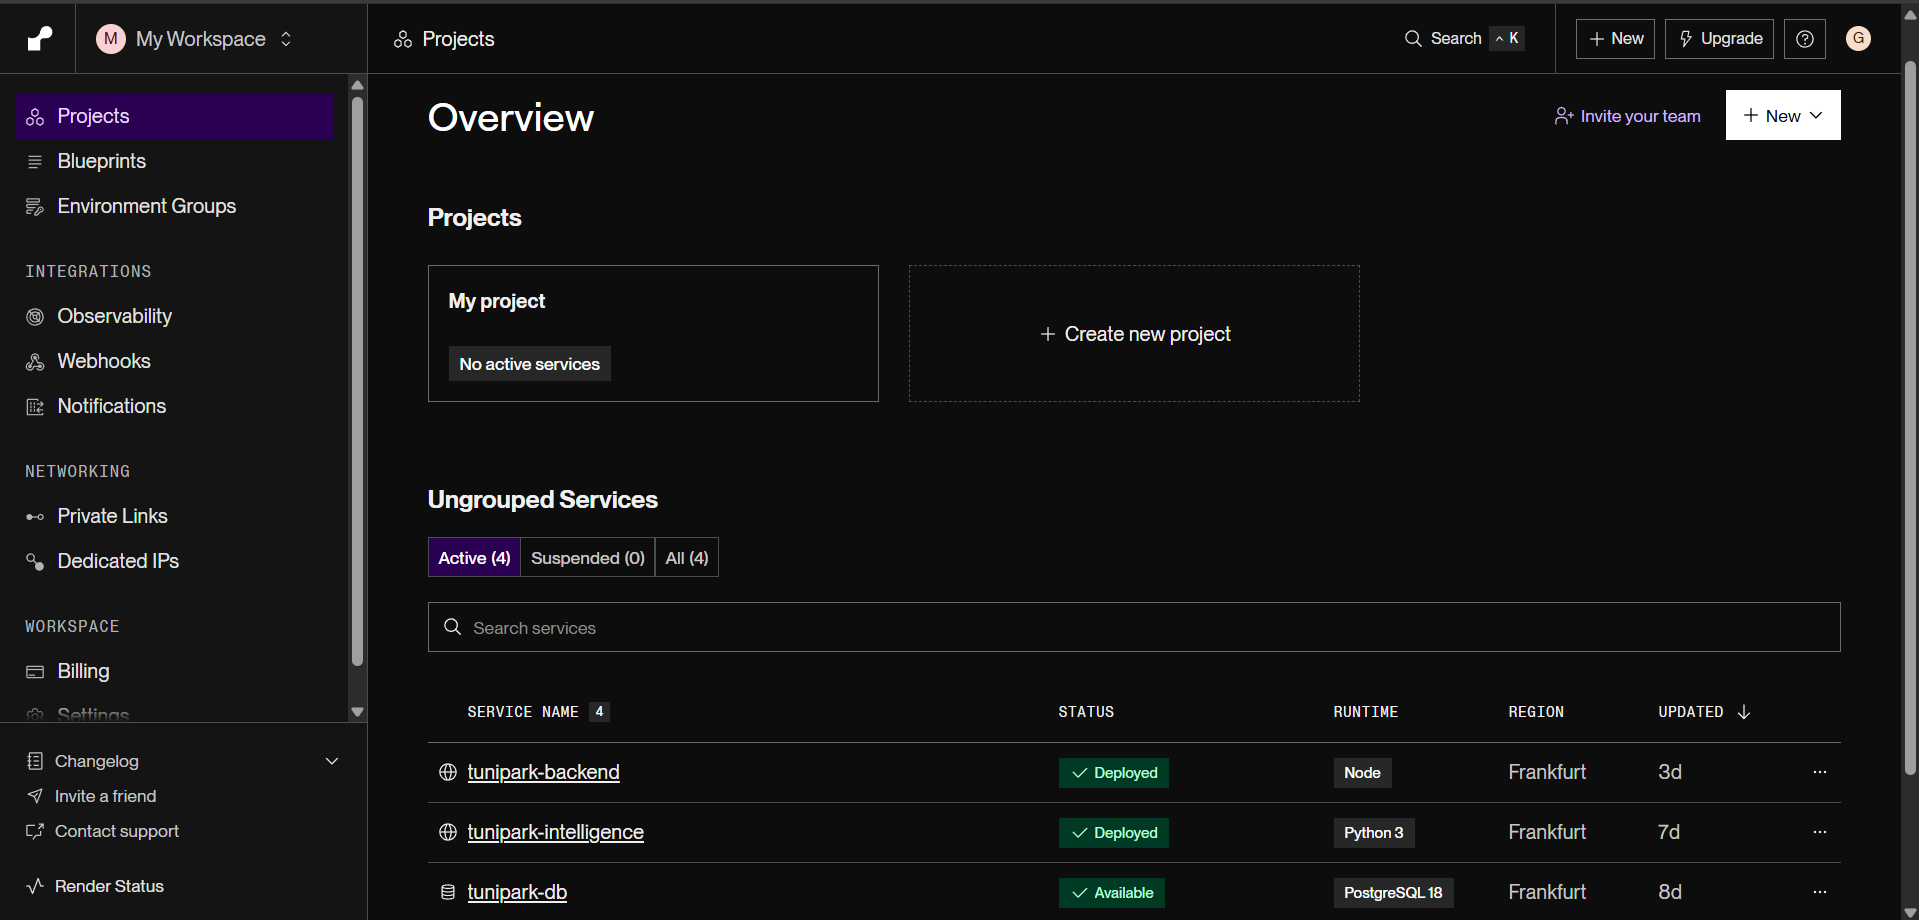
\includegraphics[width=0.95\textwidth]{img/render_dashboard.png}
    \caption{Déploiement du Backend et de la base de données sur Render}
    \label{fig:render_dashboard}
\end{figure}

\par La plateforme web d'administration développée avec \textbf{Angular} est déployée sur \textbf{Vercel}. Cette solution facilite le déploiement continu de l'application et permet la publication rapide des nouvelles versions de l'interface d'administration.

\begin{figure}[H]
    \centering
    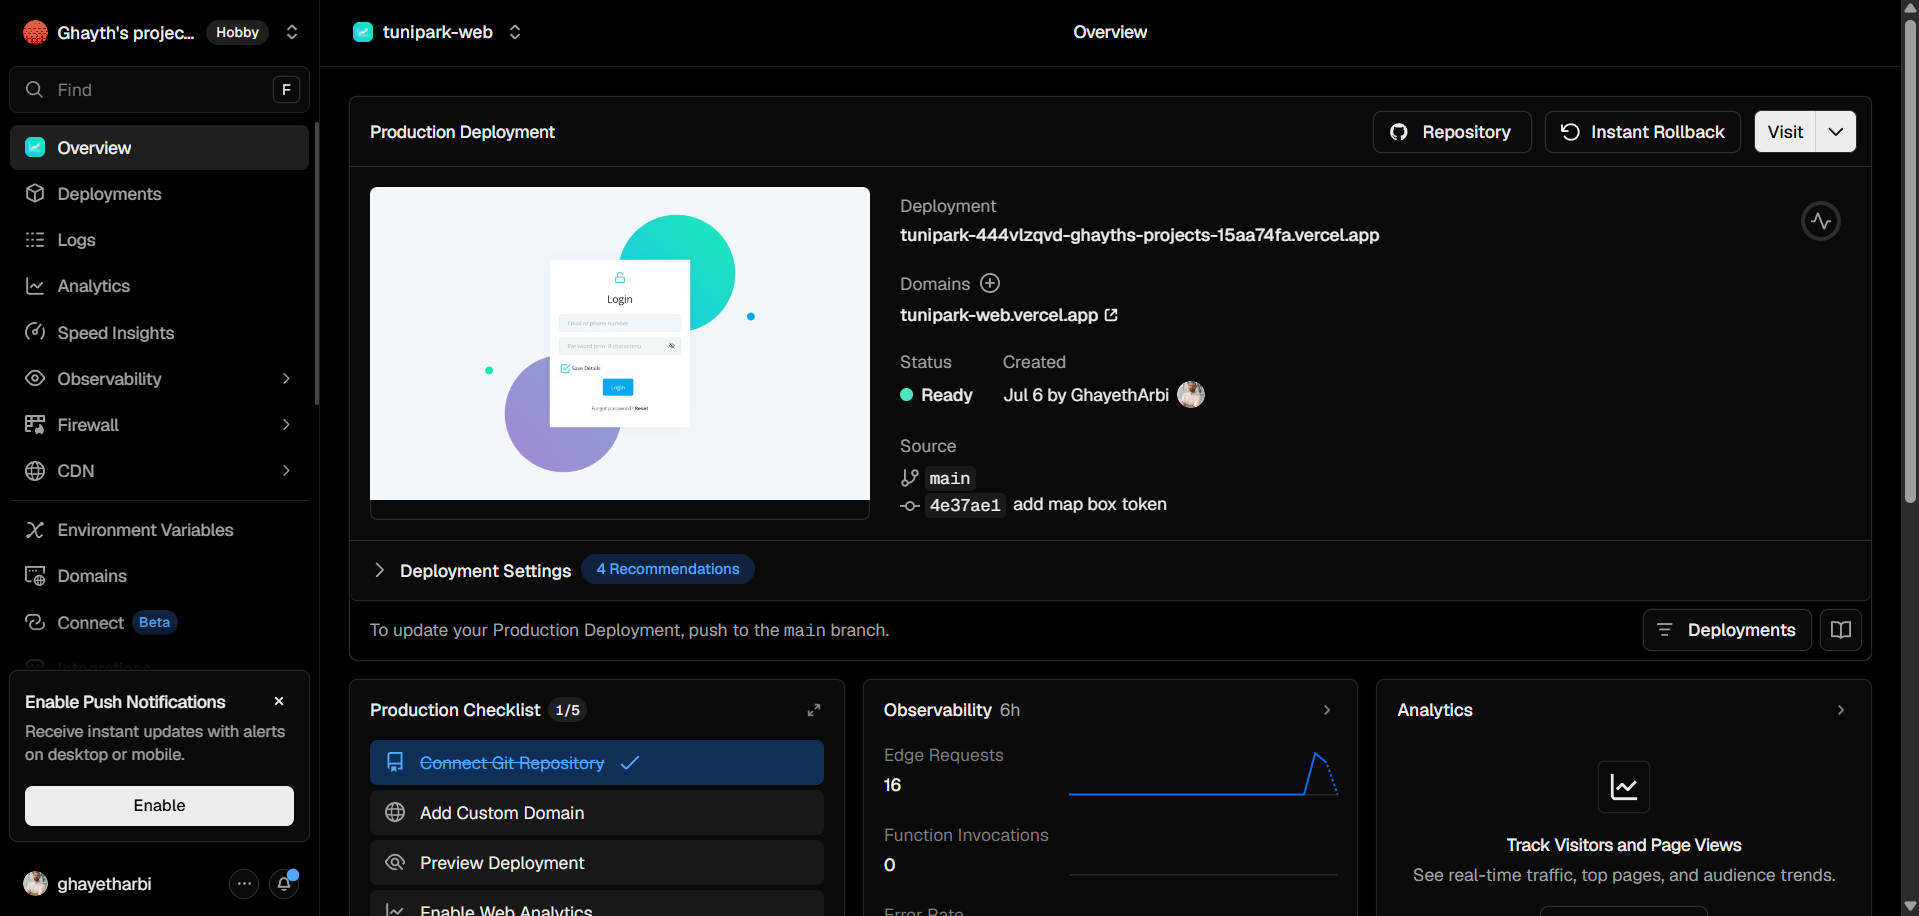
\includegraphics[width=0.95\textwidth]{img/vercel_dashboard.png}
    \caption{Déploiement de la plateforme web d'administration sur Vercel}
    \label{fig:vercel_dashboard}
\end{figure}

\par En complément de ces services, plusieurs solutions externes ont été intégrées pour garantir le fonctionnement optimal de l'application. Les images des parkings sont stockées sur \textbf{Cloudinary}, les notifications Push sont envoyées grâce à \textbf{Firebase Cloud Messaging}, les paiements électroniques sont traités par \textbf{Flouci} et les courriers électroniques sont transmis à l'aide de \textbf{Nodemailer}. L'envoi des codes OTP par SMS a été prévu via \textbf{Twilio}, mais cette fonctionnalité n'a pas été activée durant la période du projet en raison de l'absence d'un abonnement au service.

\par Cette infrastructure de déploiement permet aux différents composants de fonctionner de manière indépendante tout en garantissant une communication sécurisée entre l'application mobile, la plateforme web d'administration, le Backend, la base de données ainsi que les différents services externes intégrés à la solution.
\section{Conclusion}

\par Ce chapitre a présenté la réalisation de l'application \textbf{TuniPark} en décrivant l'environnement de développement, les principaux modules du Backend, les interfaces de l'application mobile ainsi que la plateforme web d'administration.

\par Il a également présenté les différentes fonctionnalités implémentées, notamment l'authentification sécurisée, la gestion des parkings, les sessions de stationnement, les paiements électroniques, les notifications Push et le système de recommandation intelligent basé sur un modèle Random Forest.

\par Enfin, le chapitre a décrit l'architecture de déploiement de la solution en mettant en évidence l'intégration des différents services cloud utilisés durant le projet. Le prochain chapitre portera sur tests et sur la validation de l'application afin d'évaluer son bon fonctionnement et de vérifier que les exigences définies au cours de l'analyse ont été satisfaites.
\chapter{Tests, Validation et Résultats}
\label{chap:testing_validation_results}
\section{Introduction}

\par Après l'implémentation des principaux modules de l'application \textbf{TuniPark}, une phase de tests et de validation a été réalisée afin de vérifier le bon fonctionnement des fonctionnalités développées. Cette étape avait pour objectif de s'assurer que l'application mobile, la plateforme web d'administration, les services Backend ainsi que les différents services externes fonctionnaient correctement de manière intégrée.

\par Ce chapitre présente la stratégie de test adoptée durant le développement, les outils utilisés pour la validation des API et des fonctionnalités, les principaux scénarios testés ainsi que les résultats obtenus. Il met également en évidence les difficultés rencontrées au cours de la phase de validation.

\section{Stratégie de test}

\par Les tests ont été réalisés progressivement tout au long du développement de l'application. Chaque fonctionnalité a été validée individuellement avant d'être testée après son intégration avec les autres modules. Cette approche a permis d'identifier rapidement les anomalies et de garantir le bon fonctionnement global de la plateforme.

\par La validation a principalement porté sur les fonctionnalités essentielles de TuniPark, notamment l'authentification des utilisateurs, la gestion des parkings, la création des sessions de stationnement, les paiements électroniques, les notifications Push ainsi que le système de recommandation intelligent.

\par Les principaux objectifs de cette phase de validation étaient les suivants :

\begin{itemize}
\item vérifier le bon fonctionnement de l'authentification et du contrôle d'accès ;
\item valider les opérations de gestion des parkings ;
\item confirmer le bon déroulement de la création et du paiement des sessions de stationnement ;
\item vérifier l'envoi des notifications Push ;
\item valider le fonctionnement du système de recommandation intelligent ;
\item s'assurer de la bonne communication entre les différents services de la plateforme.
\end{itemize}
\section{Outil de test des API}

\par Durant la phase de validation du Backend, l'interface \textbf{Swagger} intégrée à \textbf{NestJS} a été utilisée afin de tester directement les API développées. Cet outil a permis d'envoyer des requêtes HTTP, d'analyser les réponses du serveur et de vérifier le bon fonctionnement des différents points d'accès sans passer systématiquement par l'application mobile.

\par Dans le cadre de ce projet, Swagger \cite{swagger} a été utilisé pour tester les principales fonctionnalités de l'application, notamment l'authentification, la gestion des utilisateurs, des parkings, des sessions de stationnement, des paiements, des notifications ainsi que les routes protégées nécessitant un jeton JWT. Il a également permis de vérifier les paramètres des requêtes, les réponses retournées par le serveur ainsi que les différents codes de statut HTTP.

\begin{figure}[H]
    \centering
    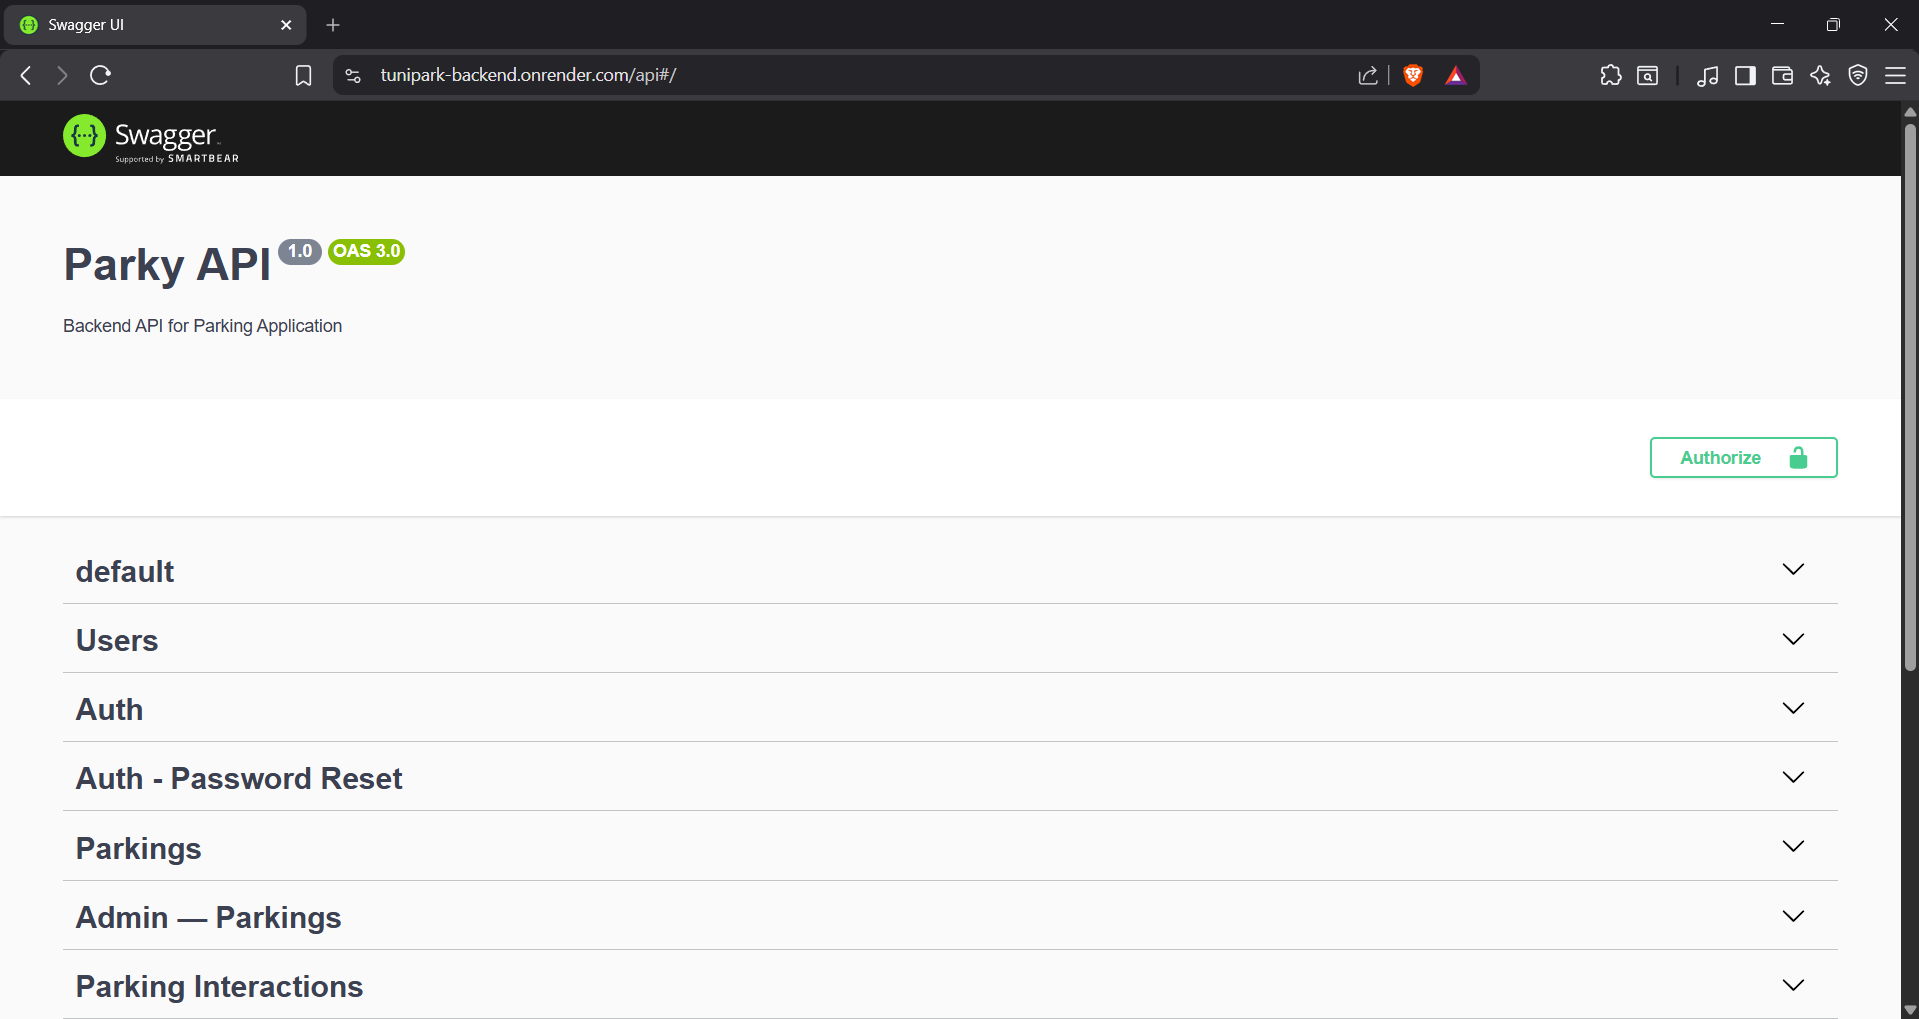
\includegraphics[width=0.9\textwidth]{img/swagger.png}
    \caption{Documentation et tests des API à l'aide de Swagger}
    \label{fig:swagger}
\end{figure}
\section{Validation des API du Backend}

\par La validation des API a débuté par le test du point d'accès d'authentification. Après une connexion réussie, le Backend génère un \textit{Access Token} ainsi qu'un \textit{Refresh Token}. Ces jetons sont ensuite utilisés pour accéder aux différentes routes sécurisées de l'application et vérifier le contrôle d'accès selon les rôles des utilisateurs.

\begin{figure}[H]
    \centering
    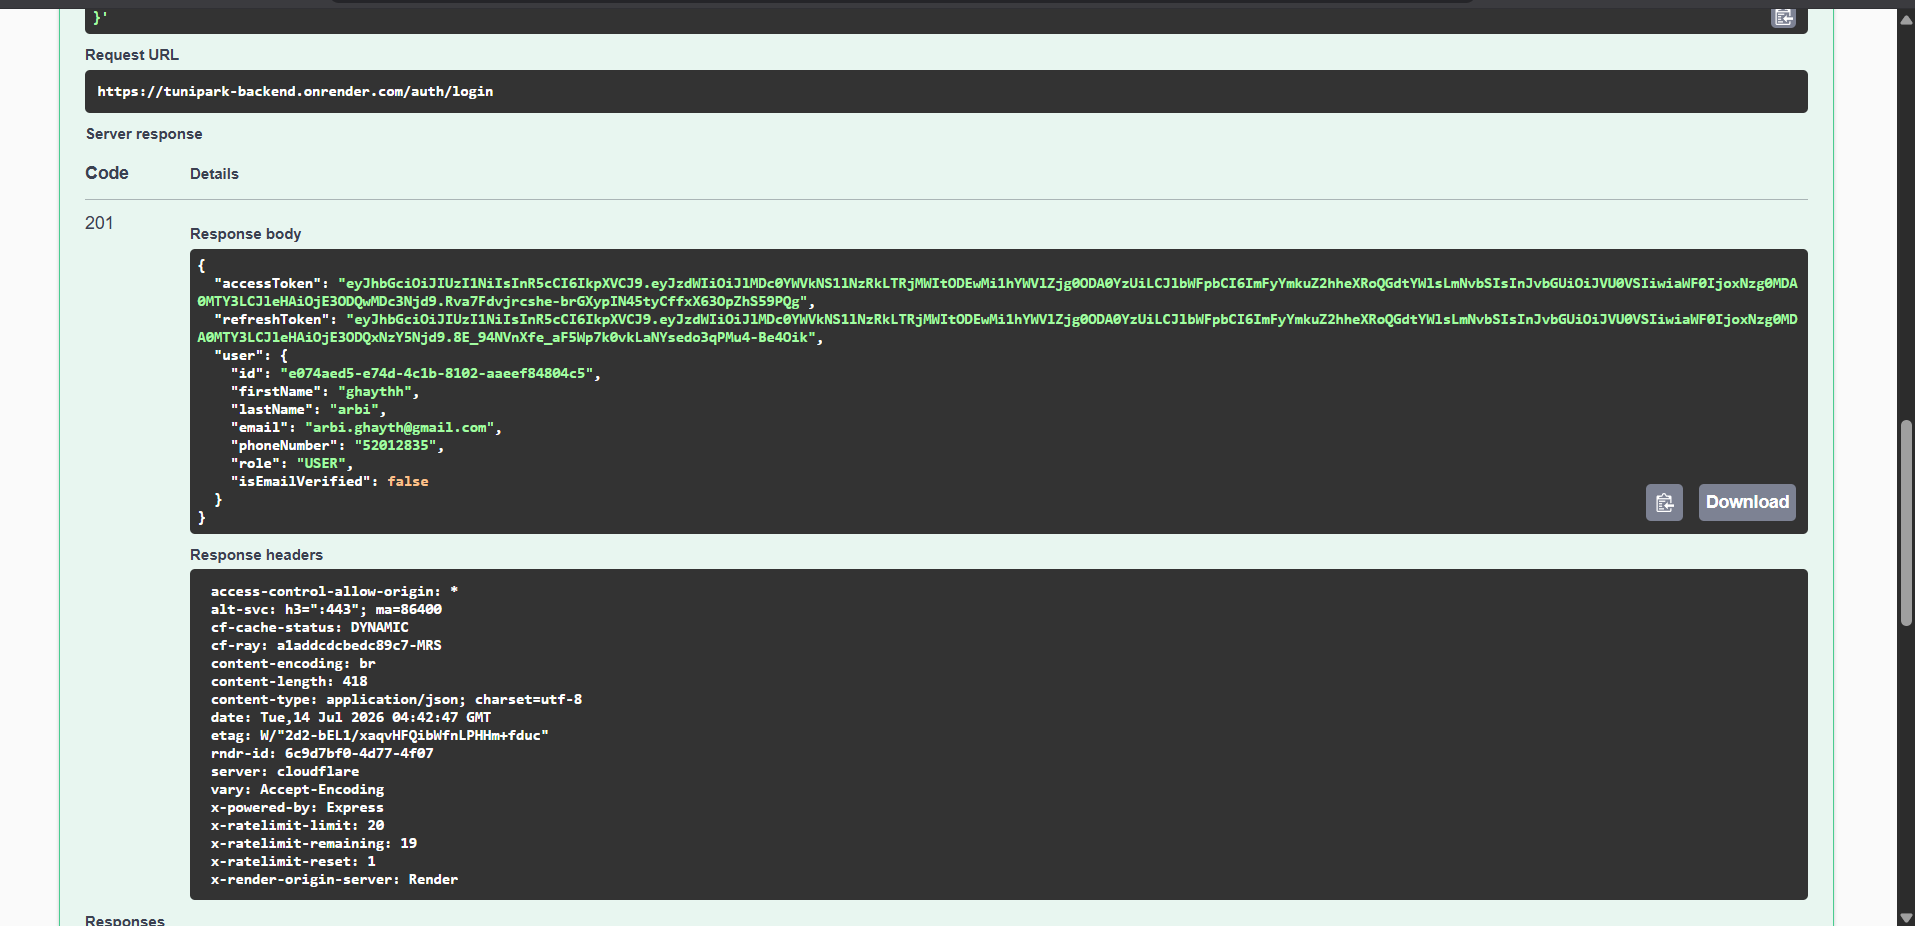
\includegraphics[width=0.95\textwidth]{img/swagger_login.png}
    \caption{Validation de l'API d'authentification avec Swagger}
    \label{fig:swagger_login_test}
\end{figure}

\par Des tests complémentaires ont ensuite été réalisés sur les principales API de l'application, notamment la gestion des parkings, la création et le paiement des sessions de stationnement, les notifications, le système de recommandation ainsi que les opérations d'administration. Ces essais ont confirmé que les requêtes valides étaient correctement traitées et que le Backend retournait les réponses ainsi que les codes d'erreur appropriés lorsque les données fournies étaient incomplètes ou invalides.

\section{Tests fonctionnels}

\par Les tests fonctionnels ont été réalisés afin de vérifier le bon fonctionnement de l'application \textbf{TuniPark} du point de vue des utilisateurs et des administrateurs. Chaque fonctionnalité a été testée dans des conditions d'utilisation réelles afin de s'assurer que les résultats obtenus correspondaient au comportement attendu.

\par Les essais ont porté sur les principales fonctionnalités de l'application, notamment l'authentification, la gestion des parkings, la création des sessions de stationnement, les paiements électroniques, les notifications Push ainsi que le système de recommandation intelligent. Les résultats obtenus ont permis de confirmer le bon fonctionnement de l'ensemble des modules développés.

\subsection{Tests d'authentification et de contrôle d'accès}

\par Les tests d'authentification ont permis de vérifier la connexion des utilisateurs, la génération des jetons JWT ainsi que le contrôle d'accès aux ressources protégées. Le mécanisme de renouvellement automatique des jetons à l'aide du \textit{Refresh Token} a également été validé.

\begin{table}[H]
\centering
\small
\renewcommand{\arraystretch}{1.25}
\begin{tabular}{|p{0.35\textwidth}|p{0.38\textwidth}|p{0.17\textwidth}|}
\hline
\textbf{Test} & \textbf{Comportement attendu} & \textbf{Résultat} \\
\hline
Connexion avec des identifiants valides & L'utilisateur accède à l'application. & Réussi \\
\hline
Connexion avec des identifiants invalides & Message d'erreur affiché. & Réussi \\
\hline
Accès sans jeton JWT & La requête est refusée. & Réussi \\
\hline
Renouvellement de l'Access Token & Un nouveau jeton est généré via le Refresh Token. & Réussi \\
\hline
\end{tabular}
\caption{Tests d'authentification et de contrôle d'accès}
\label{tab:auth_tests}
\end{table}

\subsection{Tests de gestion des parkings}

\par Les fonctionnalités de gestion des parkings ont été testées aussi bien du côté propriétaire que du côté administrateur. Les essais ont permis de vérifier la création d'un parking privé, sa validation par un administrateur ainsi que la mise à jour de ses informations.

\begin{table}[H]
\centering
\small
\renewcommand{\arraystretch}{1.25}
\begin{tabular}{|p{0.35\textwidth}|p{0.38\textwidth}|p{0.17\textwidth}|}
\hline
\textbf{Test} & \textbf{Comportement attendu} & \textbf{Résultat} \\
\hline
Ajouter un parking privé & Parking créé avec le statut \texttt{PENDING}. & Réussi \\
\hline
Valider un parking & Le statut devient \texttt{ACTIVE}. & Réussi \\
\hline
Rejeter un parking & Le parking reste indisponible. & Réussi \\
\hline
Modifier les informations d'un parking & Les modifications sont enregistrées. & Réussi \\
\hline
\end{tabular}
\caption{Tests de gestion des parkings}
\label{tab:parking_tests}
\end{table}

\subsection{Tests des sessions de stationnement et des paiements}

\par Les scénarios de création d'une session de stationnement et de paiement via Flouci ont été validés afin de vérifier le bon déroulement du processus complet.

\begin{table}[H]
\centering
\small
\renewcommand{\arraystretch}{1.25}
\begin{tabular}{|p{0.35\textwidth}|p{0.38\textwidth}|p{0.17\textwidth}|}
\hline
\textbf{Test} & \textbf{Comportement attendu} & \textbf{Résultat} \\
\hline
Créer une session & Une session est créée avec le statut \texttt{CREATED}. & Réussi \\
\hline
Paiement Flouci validé & La session passe au statut \texttt{ACTIVE}. & Réussi \\
\hline
Paiement annulé & La session n'est pas activée. & Réussi \\
\hline
Fin de session & Le paiement est enregistré correctement. & Réussi \\
\hline
\end{tabular}
\caption{Tests des sessions de stationnement et des paiements}
\label{tab:session_tests}
\end{table}

\subsection{Tests des notifications}

\par Les notifications internes ainsi que les notifications Push envoyées via Firebase Cloud Messaging ont été testées afin de vérifier leur création, leur envoi et leur affichage dans l'application.

\begin{table}[H]
\centering
\small
\renewcommand{\arraystretch}{1.25}
\begin{tabular}{|p{0.35\textwidth}|p{0.38\textwidth}|p{0.17\textwidth}|}
\hline
\textbf{Test} & \textbf{Comportement attendu} & \textbf{Résultat} \\
\hline
Créer une notification & Notification enregistrée en base de données. & Réussi \\
\hline
Notification Push FCM & Réception sur le téléphone mobile. & Réussi \\
\hline
Marquer une notification comme lue & Mise à jour du statut de lecture. & Réussi \\
\hline
\end{tabular}
\caption{Tests des notifications}
\label{tab:notification_tests}
\end{table}

\subsection{Tests du système de recommandation}

\par Le système de recommandation intelligent a été testé afin de vérifier le fonctionnement du modèle Random Forest et la génération des recommandations de parkings.

\begin{table}[H]
\centering
\small
\renewcommand{\arraystretch}{1.25}
\begin{tabular}{|p{0.35\textwidth}|p{0.38\textwidth}|p{0.17\textwidth}|}
\hline
\textbf{Test} & \textbf{Comportement attendu} & \textbf{Résultat} \\
\hline
Demande de recommandations & Liste des parkings recommandés affichée. & Réussi \\
\hline
Microservice IA disponible & Calcul des scores avec Random Forest. & Réussi \\
\hline
Indisponibilité du microservice & Utilisation de l'algorithme de secours. & Réussi \\
\hline
\end{tabular}
\caption{Tests du système de recommandation}
\label{tab:ai_tests}
\end{table}


\section{Validation de la base de données}

\par La validation de la base de données \textbf{PostgreSQL} a été réalisée en vérifiant que les différentes opérations effectuées depuis l'application entraînaient bien les modifications attendues au niveau des données. Les résultats obtenus ont été contrôlés à travers les réponses des API ainsi que les journaux d'exécution du Backend.

\par Les contrôles ont principalement concerné la mise en place des comptes utilisateurs, l'intégration et l'approbation des parkings, l'établissement des sessions de stationnement, le suivi des paiements, les alertes, ainsi que les communications employées par le système de recommandation. Les différents tests ont confirmé que les opérations de création, de modification et de suppression étaient correctement prises en compte et que la cohérence entre les entités associées était bien préservée.
\begin{figure}[H]
    \centering
    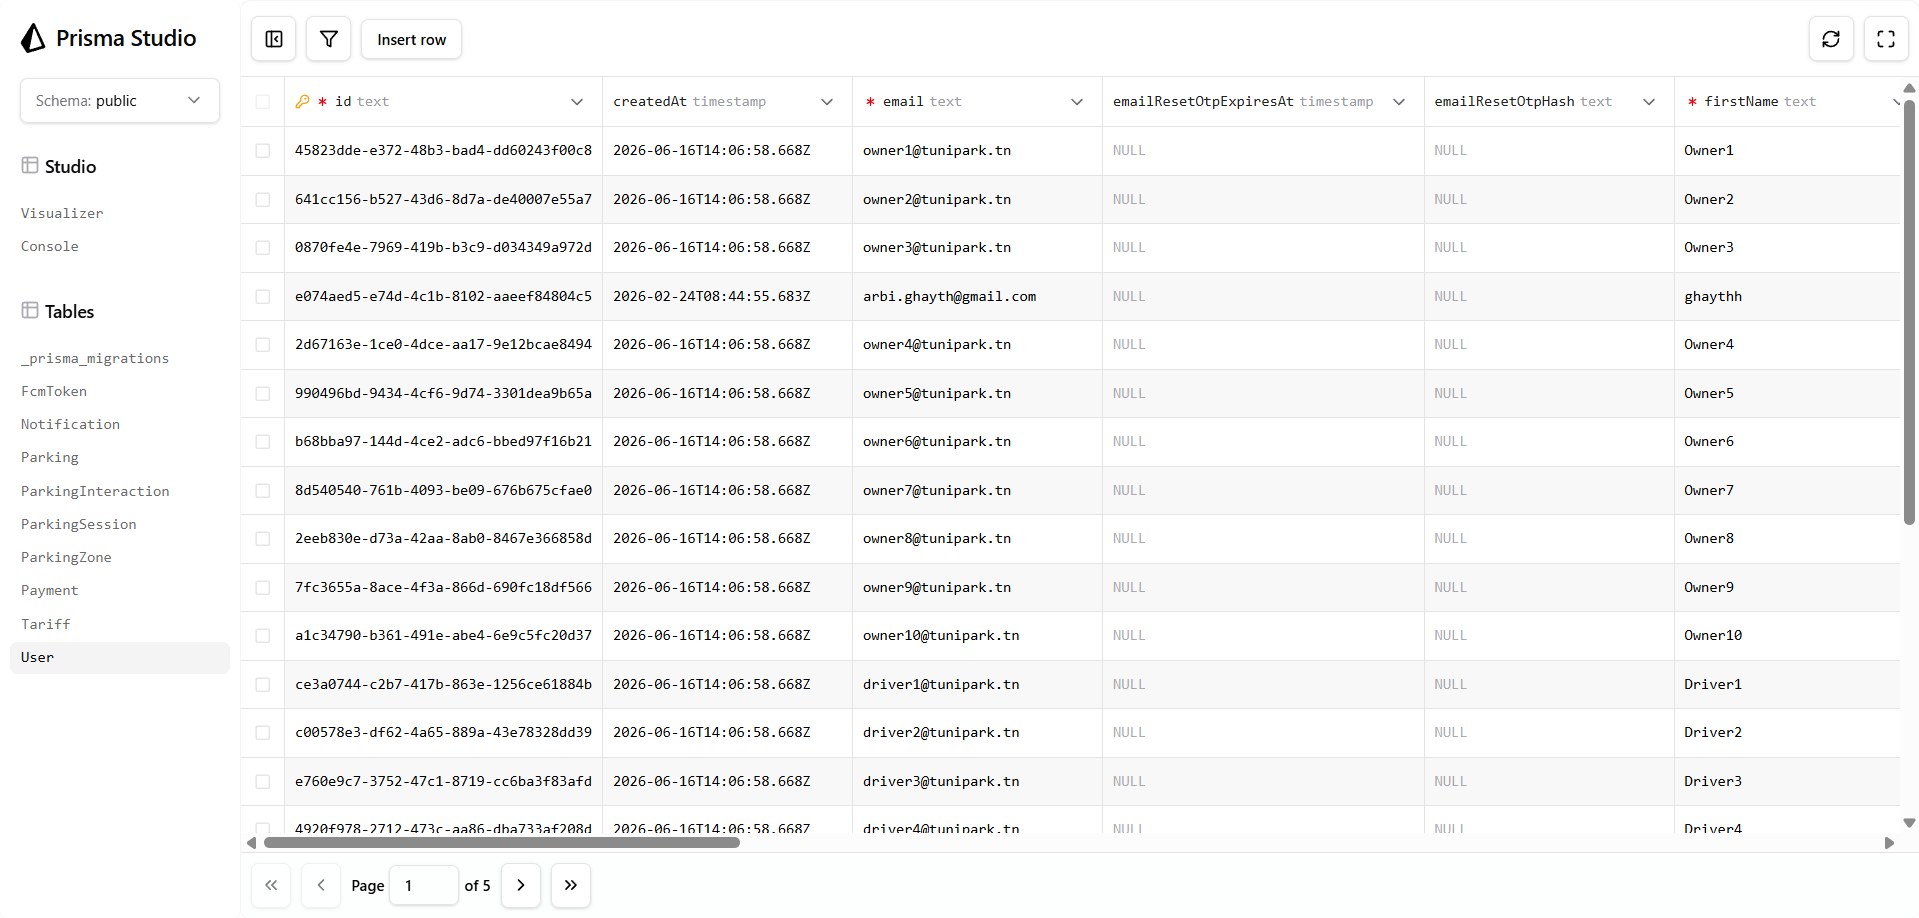
\includegraphics[width=0.95\textwidth]{img/postgresql_validation.png}
    \caption{Validation des données enregistrées dans PostgreSQL}
    \label{fig:postgres_validation}
\end{figure}


\section{Validation des services externes}

\par Plusieurs fonctionnalités de l'application \textbf{TuniPark} reposent sur des services externes. Des tests ont donc été réalisés afin de vérifier leur bonne intégration avec le Backend. Les validations ont principalement concerné le paiement électronique avec \textbf{Flouci}, l'envoi des notifications Push via \textbf{Firebase Cloud Messaging} ainsi que le stockage des images sur \textbf{Cloudinary}.

\subsection{Validation des paiements avec Flouci}

\par L'intégration de Flouci a été validée lors de la création d'une session de stationnement. Après la sélection d'un parking, l'utilisateur a été redirigé vers la plateforme de paiement. Une fois la transaction confirmée, Flouci a transmis le résultat au Backend, qui a mis à jour le statut du paiement ainsi que celui de la session de stationnement.

\begin{figure}[H]
    \centering
    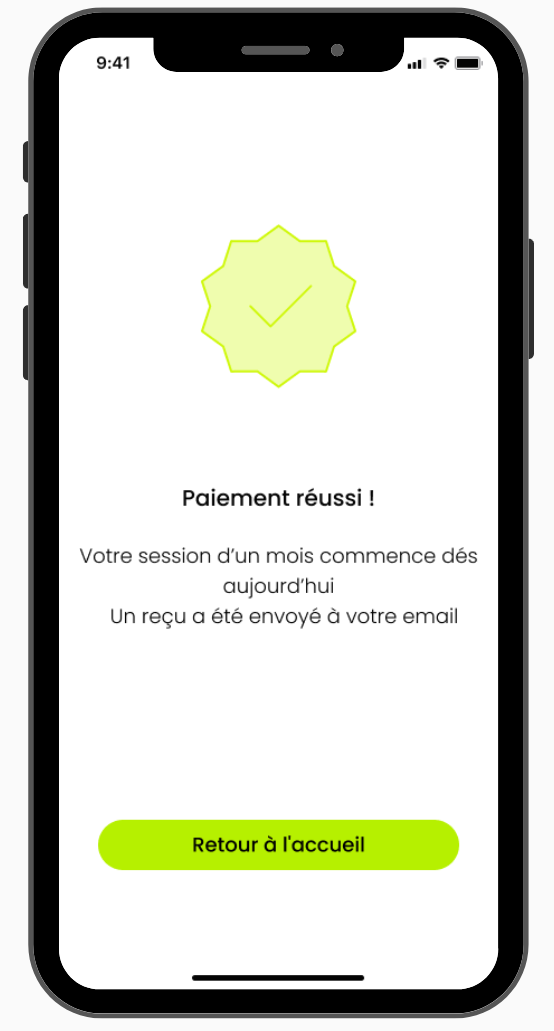
\includegraphics[width=0.5\textwidth]{img/flouci_test.png}
    \caption{Validation d'un paiement avec Flouci}
    \label{fig:flouci_test}
\end{figure}

\par Les essais réalisés ont confirmé le bon fonctionnement du processus de paiement et la mise à jour correcte des informations enregistrées dans la base de données.

\subsection{Validation des notifications Firebase}

\par Les notifications Push ont été testées à l'aide de Firebase Cloud Messaging. Lorsqu'un événement nécessitant une notification se produit, le Backend récupère le jeton FCM de l'utilisateur et transmet la notification au service Firebase, qui l'envoie ensuite vers l'appareil mobile.

\begin{figure}[H]
    \centering
    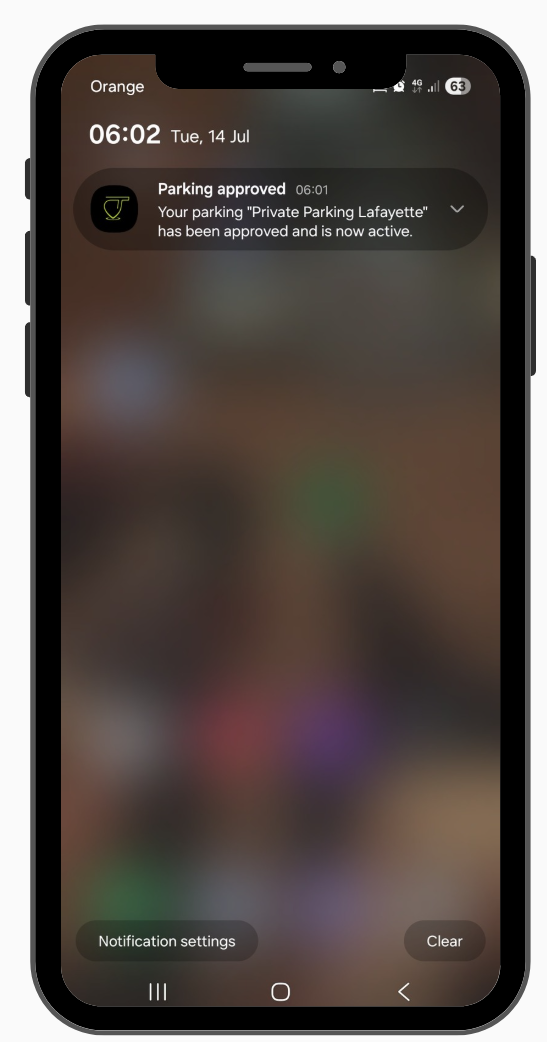
\includegraphics[width=0.45\textwidth]{img/firebase_test.png}
    \caption{Validation des notifications Push avec Firebase Cloud Messaging}
    \label{fig:firebase_test}
\end{figure}

\par Les notifications ont été correctement reçues sur les appareils de test et enregistrées dans l'application.

\subsection{Validation du stockage Cloudinary}

\par Le service Cloudinary a été utilisé pour stocker les images des parkings ajoutées par les propriétaires. Les tests ont consisté à téléverser plusieurs images depuis l'application puis à vérifier leur enregistrement sur Cloudinary ainsi que leur affichage après récupération par le Backend.

\begin{figure}[H]
    \centering
    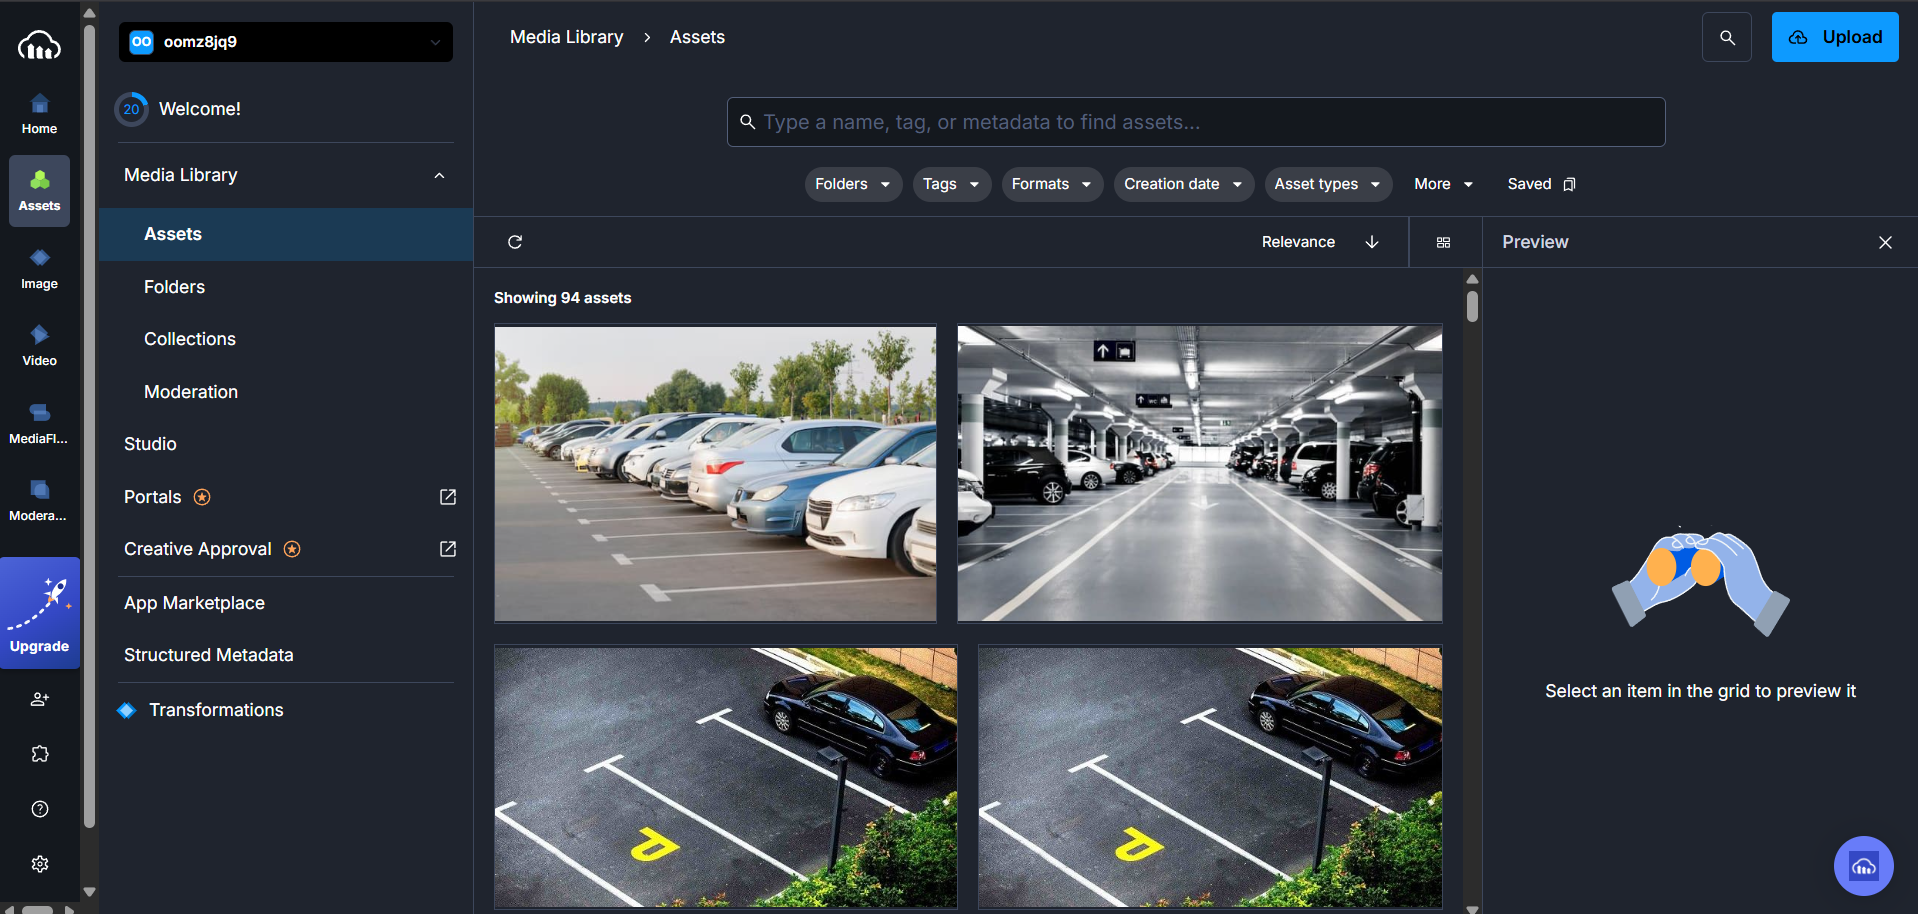
\includegraphics[width=0.9\textwidth]{img/cloudinary_test.png}
    \caption{Validation du stockage des images avec Cloudinary}
    \label{fig:cloudinary_test}
\end{figure}

\par Les essais ont confirmé que les images étaient correctement téléversées, stockées puis affichées dans l'application sans perte de qualité.
\section{Résultats et discussion}

\par Les différentes phases de validation ont confirmé le bon fonctionnement des principales fonctionnalités de l'application \textbf{TuniPark}. Les utilisateurs peuvent créer un compte, s'authentifier de manière sécurisée, consulter les parkings disponibles, démarrer une session de stationnement, effectuer un paiement électronique, recevoir des notifications Push et bénéficier du système de recommandation intelligent. Les propriétaires peuvent proposer leurs parkings privés, tandis que les administrateurs disposent des outils nécessaires pour les valider et assurer la gestion de la plateforme.

\par Les tests ont également permis de vérifier le bon fonctionnement des échanges entre les différents composants de la solution. Le Backend assure la sécurisation des requêtes grâce à l'authentification JWT, communique correctement avec la base de données PostgreSQL et s'intègre aux différents services externes tels que Flouci, Firebase Cloud Messaging et Cloudinary. Le système de recommandation basé sur le modèle Random Forest fournit des recommandations cohérentes en fonction des caractéristiques des parkings et des préférences de l'utilisateur.

\par Malgré les résultats obtenus, certaines améliorations peuvent être envisagées. Parmi celles-ci figurent l'optimisation des performances du système de recommandation à partir d'un plus grand volume de données, l'activation de la vérification des numéros de téléphone par SMS via Twilio, ainsi que l'ajout de nouvelles fonctionnalités de gestion et d'analyse destinées aux administrateurs.

\section{Conclusion}

\par Ce chapitre a présenté les différentes activités de validation réalisées sur l'application \textbf{TuniPark}. Il a couvert les tests des API du Backend, les tests fonctionnels, la validation de la base de données ainsi que la vérification des principaux services externes intégrés à la solution.

\par Les résultats obtenus montrent que les différentes fonctionnalités développées répondent aux exigences définies lors de l'analyse des besoins. Les tests réalisés ont confirmé la fiabilité des principaux modules de l'application, notamment l'authentification, la gestion des parkings, les sessions de stationnement, les paiements électroniques, les notifications Push et le système de recommandation intelligent.

\par Ce travail fournit un socle robuste pour les futures améliorations de l'application. Les améliorations possibles sont exposées dans la conclusion générale de ce travail de recherche.
\chapter*{Conclusion Générale et Perspectives}
\addcontentsline{toc}{chapter}{Conclusion Générale et Perspectives}

\section*{Conclusion Générale}

\par Ce projet de fin d'études a permis de concevoir et de développer \textbf{TuniPark}, une application intelligente de gestion du stationnement destinée à faciliter la recherche, la réservation et le paiement des places de stationnement. La solution proposée répond aux difficultés rencontrées par les automobilistes lors de la recherche d'une place disponible, tout en offrant aux propriétaires de parkings privés un moyen simple de proposer leurs emplacements et de les gérer efficacement.

\par Le projet a débuté par une étude du contexte général du stationnement ainsi que par une analyse des besoins des différents acteurs. Cette phase a permis d'identifier les exigences fonctionnelles et non fonctionnelles du système, de définir les cas d'utilisation et d'établir le Product Backlog ayant servi de base à la réalisation de l'application.

\par La phase de conception a permis de définir l'architecture générale de la solution à travers les architectures logique et physique ainsi que les différents diagrammes UML. Les choix technologiques se sont appuyés sur \textbf{Flutter} pour le réalisation  de l'application mobile, \textbf{NestJS} pour le Backend, \textbf{PostgreSQL} pour le stockage des données et \textbf{Angular} pour la plateforme web d'administration. Plusieurs services externes ont également été intégrés, notamment \textbf{Flouci} pour les paiements électroniques, \textbf{Firebase Cloud Messaging} pour les notifications Push et \textbf{Cloudinary} pour le stockage des images.

\par La phase d'implémentation a conduit au développement d'une application complète intégrant l'authentification sécurisée, la gestion des parkings publics et privés, la création des sessions de stationnement, le paiement électronique, les notifications Push ainsi qu'une plateforme web destinée à l'administration des parkings et des utilisateurs. Une attention particulière a également été portée au développement d'un système de recommandation intelligent reposant sur un modèle de \textbf{Random Forest}, permettant de proposer aux utilisateurs les parkings les plus adaptés à leur situation.

\par Enfin, les différentes phases de validation ont confirmé le bon fonctionnement des principaux modules de l'application. Les tests des API, les tests fonctionnels ainsi que la validation des services externes ont permis de vérifier la fiabilité de la solution développée et de s'assurer que les principales exigences définies au début du projet étaient satisfaites.

\section*{Perspectives}

\par Plusieurs améliorations pourront être apportées aux futures versions de \textbf{TuniPark}. Une première évolution consistera à enrichir le système de recommandation en exploitant un volume plus important de données réelles afin d'améliorer la précision des suggestions proposées aux utilisateurs. L'intégration de techniques d'apprentissage plus avancées et la prise en compte des habitudes de stationnement permettraient d'obtenir des recommandations encore plus pertinentes.

%\par Une autre perspective concerne l'amélioration des fonctionnalités de réservation. Il serait intéressant d'ajouter un système de réservation anticipée avec une durée configurable, ainsi qu'un mécanisme de tarification dynamique tenant compte de la demande, des horaires et du taux d'occupation des parkings.

\par L'application pourrait également intégrer de nouveaux moyens de paiement ainsi que l'activation complète de la vérification des numéros de téléphone par SMS à l'aide de \textbf{Twilio}. Cette fonctionnalité renforcerait la sécurité des comptes utilisateurs et simplifierait les procédures de récupération d'accès.

\par Enfin, plusieurs fonctionnalités destinées aux administrateurs et aux propriétaires de parkings pourraient être développées, telles que des tableaux de bord statistiques plus avancés, l'analyse de l'occupation des parkings en temps réel, la génération automatique de rapports ainsi que des outils d'aide à la décision permettant d'optimiser la gestion des espaces de stationnement.

% IEEE style is very common in electrical engineering, computer science, and related fields. 
% It uses a numbered citation system within square brackets in the text, with a numerically ordered bibliography at the end.
\bibliographystyle{IEEEtran} 
\bibliography{references}


\includepdf[pages=1]{Page_Garde.pdf}

\end{document}